\documentclass[11.5pt, twoside, a4paper, titlepage]{report}
\usepackage{graphicx, amssymb, amsmath, mathtools, amsthm, xfrac, mathabx, upgreek}
\usepackage{tikz}
\usetikzlibrary{automata, arrows, matrix}
\providecommand{\abs}[1]{\lvert#1\rvert}
\providecommand{\bb}[1]{\mathbb{#1}}
\theoremstyle{definition}
\newtheorem{mydef}{Definition}[section]
\newtheorem{rem}[mydef]{Remark}
\newtheorem{note}[mydef]{Notation}
\newtheorem{eg}[mydef]{Example}
\theoremstyle{plain}
\newtheorem{lem}[mydef]{Lemma}
\newtheorem{thm}[mydef]{Theorem}
\newtheorem{cor}[mydef]{Corollary}
\newtheorem{prop}[mydef]{Proposition}
\newtheorem*{claim}{Claim}
\newtheorem*{wrong}{Wrong Definition}
\newcommand{\mytab}[1]{%
\begin{tabular}{@{}c@{}}
#1
\end{tabular}
}


\begin{document}
\title{Representation of Quivers}
\author{Chanelle Lee \\Student ID: 200646370\\Supervisor: William Crawley-Boevey}
\date{\today}
\maketitle


\tableofcontents

\chapter{Introduction}

This project aims to cover interesting topics from the area of quiver representations. The first chapter will give a brief introduction to the topics in Homological Algebra needed for bulk of the report. It will cover chain complexes, exact sequences, short exact sequences, and extensions, most importantly $Ext^1$. The the second chapter will introduce quivers and look at some interesting results about path algebras before moving onto representations of quivers and their relationship with the modules of the corresponding path algebra. Next we will cover Dynkin and Euclidean diagrams before finishing with a proof of Gabriel's Theorem. The third chapter will cover Auslander-Reiten quivers.

\chapter{Homological Algebra}

In this chapter we will be introducing results from Homological Algebra and will mainly be following the first two sections of \cite{CB1}, but with heavy influence from \cite{Rotman} and \cite{Weibel}. We will first explore chain complexes before moving onto exact sequences and extensions before finishing by looking at some results of $Ext^1$ will be useful later on in the report. For the chapter, we let $R$ be a ring and will be considering left $R$-modules.

%%%%%%%%%%%%%%%%%%%%%%%%%%%%%%%%%%%%%%%%%%%%%%%%%%%%%%%
%%%%%%%%%%%%%%			CHAIN COMPLEXES 		%%%%%%%%%%%%%%%%%%%%
%%%%%%%%%%%%%%%%%%%%%%%%%%%%%%%%%%%%%%%%%%%%%%%%%%%%%%%
\section{Chain Complexes}

\begin{mydef}
A \emph{chain complex} $\mathbf{C}_{\bullet}$ consists of a sequence of $R$-modules $C_i$ ($i \in \mathbb{Z}$) and morphisms of the form,
\begin{equation*}
\mathbf{C}: \qquad \dots \xrightarrow{\delta_{3}} C_2 \xrightarrow{\delta_{2}} C_1 \xrightarrow{\delta_{1 }} C_0 \xrightarrow{\delta_0} C_{-1} \xrightarrow{\delta_{-1}} C_{-2} \xrightarrow{\delta_{-2}}\dots
\end{equation*}
such that $\delta_{n-1}\delta_{n}=0$ for all $n$, i.e. the composition of any two consecutive maps is zero. The maps $\delta_n$ are called the \emph{differentials} of $C$.
\end{mydef}

\begin{rem}
It is convention that the map $\delta_n$ starts at $C_n$.
\end{rem}

\begin{eg}
If we have a field $k$ then we can create the following chain complex:
\begin{equation*}
\mathbf{C}: \qquad \dots \xrightarrow{} 0 \xrightarrow{} k^2 \xrightarrow{\Bigl(\begin{smallmatrix}1&2\\ 3&0\\ 0&0 \end{smallmatrix}\Bigr)} k^3 \xrightarrow{(\begin{smallmatrix}0 & 0 &1\end{smallmatrix})} k \xrightarrow{} 0 \xrightarrow{}\dots
\end{equation*}
We can clearly see that the maps uphold the $\delta^2=0$ condition as,
\begin{equation*}
\begin{pmatrix}0 & 0 &1
\end{pmatrix}
\begin{pmatrix}
1 & 2 \\
3 & 0\\
0 & 0
\end{pmatrix}
=\begin{pmatrix}
0 & 0
\end{pmatrix}.
\end{equation*}
\end{eg}

\begin{eg} \label{kchaineg}
If we consider the sequence, 
\begin{equation*} 
\dots \xrightarrow{} 0 \xrightarrow{} k \xrightarrow{\delta_2=\big(\begin{smallmatrix} 1\\ 0 \end{smallmatrix}\big)} k^2 \xrightarrow{\delta_1=(\begin{smallmatrix}1 & 0 \end{smallmatrix})} k \xrightarrow{} 0 \xrightarrow{} \dots
\end{equation*}
however,
\begin{equation*}
\begin{pmatrix}
1 & 0
\end{pmatrix}
\begin{pmatrix*}
1\\
0
\end{pmatrix*}
= 1 \neq 0.
\end{equation*}
Hence, $\delta_1\delta_2 \neq0$, and so the sequence is not a chain complex. However, if we change $\delta_2$ slightly we obtain the chain complex,
\begin{equation*}
\mathbf{C}: \qquad \dots \xrightarrow{} 0 \xrightarrow{} k \xrightarrow{\big(\begin{smallmatrix} 1\\ 0 \end{smallmatrix}\big)} k^2 \xrightarrow{(\begin{smallmatrix}0 & 1 \end{smallmatrix})} k \xrightarrow{} 0 \xrightarrow{} \dots
\end{equation*}
since, 
\begin{equation*}
\begin{pmatrix}
1 & 0
\end{pmatrix}
\begin{pmatrix*}
0\\
1
\end{pmatrix*}
= 1 \neq 0.
\end{equation*}
\end{eg}

\begin{mydef}
For a chain complex,
\begin{equation*}
\mathbf{C}: \qquad \dots \xrightarrow{} C_{n+1} \xrightarrow{\delta_{n+1 }} C_{n} \xrightarrow{\delta_{n}} C_{n-1} \xrightarrow{} \dots
\end{equation*}
we define:
\begin{equation*}
Z_n(\mathbf{C})=ker(\delta_n) \quad \& \quad B_n(\mathbf{C})=im(\delta_{n+1}).
\end{equation*}
\end{mydef}

To explore the relationship between $Z_n(\mathbf{C})$ and $B_n(\mathbf{C})$, the following is a solution to Exercise 2.14 in \cite{Rotman}.(Note the example will not be provided here as exactness has not yet been covered.)

\begin{lem}\label{iminkerlem}
Let,
\begin{equation*}
A \xrightarrow{f} B \xrightarrow{g} C,
\end{equation*}
be a sequence of module maps. Then $gf=0$ if and only if $im(f)\subseteq im(g)$.
\end{lem}
\begin{proof}
Suppose $gf=0$, i.e., for all $a\in A$, $g(f(a))=0$ which implies that $f(a)\in ker(g)$ for all $a \in A$. Hence, $im(f) \subseteq ker(g)$.\\
Conversely, suppose that $im(f) \subseteq ker(g)$. Every element $b\in im(f)$ is also an element of $ker(g)$, thus $gf=0$.
\end{proof}

\begin{mydef} \label{homologydefn}
If $\mathbf{C}$ is a chain complex then its \emph{homology} is defined to be,
\begin{equation*}
H_n(\mathbf{C})=\frac{ker(\delta_n:C_n \rightarrow C_{n-1})}{im(\delta_{n+1}:C_{n+1} \rightarrow C_n)}=\frac{Z_n(\mathbf{C})}{B_n(\mathbf{C})},
\end{equation*}
which is an R-module.
\end{mydef}


The subsequent proposition is the solution to Exercise 6.1 in \cite{Rotman}.

\begin{prop}
If $\mathbf{C}$ is a chain complex with $C_n=0$ for some $n$ then $H_n(\mathbf{C})=0$.
\end{prop}
\begin{proof}
Well suppose we have such a chain complex, 
\begin{equation*}
\mathbf{C}: \qquad \dots \xrightarrow{} C_{n+1} \xrightarrow{\delta_{n+1}} 0 \xrightarrow{\delta_n} C_{n-1} \xrightarrow{} \dots
\end{equation*}
the the homology is,
\begin{equation*}
H_n(\mathbf{C})=\frac{ker(\delta_n: 0 \to C_{n-1}}{im(\delta_{n+1}: C_{n+1}\to 0)},
\end{equation*}
as the only element in $C_n$ is the zero element, and so, $H_n(\mathbf{C})=0$, as required.\\
\end{proof}

Examples \ref{chainMeg} and \ref{chainZeg} are taken from \cite{CB1} and are included here because they are felt to be the clearest at demonstrating a chain complex and homology, however, the more general statement of the second example is presented as Proposition \ref{chainhomprop} because it is an interesting result.

\begin{eg}
 \label{chainMeg}
 If we take a module $M$ then we can make a chain complex;
\begin{equation*}
\mathbf{C}: \qquad \dots \xrightarrow{} 0 \xrightarrow{} M \xrightarrow{} 0 \xrightarrow{} \dots
\end{equation*}
where $M$ is at degree $n$. Then the homology will be:
\begin{equation*}
H_i(\mathbf{C})=\begin{cases}
\frac{ker(M \rightarrow 0)}{im(0 \rightarrow M)}=M & i=n,\\
0 & \text{otherwise}.
\end{cases}
\end{equation*}
\end{eg}

\begin{rem}
Recall, 
\begin{equation*}
Coker(f)= \frac{\text{Codomain of }f}{\text{Image of }f},
\end{equation*}
is the \emph{cokernel} of the map $f$.
\end{rem}

\begin{prop}  \label{chainhomprop}
If we have a module homomorphism between $R$-modules, $f: M \xrightarrow{} N$, the we get the chain complex,
\begin{equation*}
\mathbf{C}: \qquad \underset{\text{deg}}{\dots} \xrightarrow{}\underset{n+2}{0} \xrightarrow{} \underset{n+1}{M} \xrightarrow{f}\underset{n}{N} \xrightarrow{} \underset{n-1}{0} \xrightarrow{}\dots ,
\end{equation*}
and the homology becomes,
\begin{equation*}
H_i(\mathbf{C})=
\begin{cases}
\frac{N}{im(f)}=coker(f) & i=n\\
ker(f) & i=n+1\\
0 & \text{otherwise}.
\end{cases}
\end{equation*}
\end{prop}
\begin{proof}
Firstly, at degree $n$ we have that,
\begin{equation*}
H_n(\mathbf{C})=\frac{ker(N\xrightarrow{}0)}{im(M\xrightarrow{f}N)}=\frac{N}{im(f)}=coker(f).
\end{equation*}
Then at degree $n+1$ we have that,
\begin{equation*}
H_{n+1}(\mathbf{C})=\frac{ker(M\xrightarrow{f}N)}{im(0\xrightarrow{}M)}=ker(f).
\end{equation*}
Finally, it is clear that everywhere else there is no homology.
\end{proof}

\begin{rem}
Recall, 
\begin{equation*}
Coker(f)= \frac{\text{Codomain of }f}{\text{Image of }f},
\end{equation*}
is the \emph{cokernel} of the map $f$.
\end{rem}

\begin{eg} \label{chainZeg}
We can have a chain complex of $\mathbb{Z}$-modules,
\begin{equation*}
\mathbf{C}: \qquad \underset{\text{deg}}{\dots} \xrightarrow{}\underset{2}{0} \xrightarrow{} \underset{1}{\mathbb{Z}} \xrightarrow{a}\underset{0}{\mathbb{Z}} \xrightarrow{} \underset{-1}{0} \xrightarrow{}\dots 
\end{equation*}
where the map $a$ is right multiplication by some $a \in \mathbb{Z}$. Firstly, we deal with the case where $a$ is not the zero map. \\
The homology is,
\begin{equation*}
H_i(\mathbf{C}) = 
\begin{cases}
\frac{ker(\mathbb{Z}\xrightarrow{} 0)}{im(\mathbb{Z}\xrightarrow{a}\mathbb{Z})}=\frac{\mathbb{Z}}{a\mathbb{Z}} & i=0,\\
0 & \text{otherwise}.
\end{cases}
\end{equation*}
Note that,
\begin{equation*}
H_0(\mathbf{C})=\frac{\bb{Z}}{a\bb{Z}}= \frac{\text{Codomain of }f}{\text{Image of }f}=coker(a).
\end{equation*}
Also,
\begin{equation*}
H_1(\mathbf{C})=\frac{ker(\bb{Z}\xrightarrow{a}\bb{Z})}{im(0\xrightarrow{}\bb{Z})}=ker(a)=0,
\end{equation*}
as $a$ is injective.\\
However, in the instance that $a$ is the zero map, we have that,
\begin{equation*}
ker(\bb{Z} \xrightarrow{0} \bb{Z})=\bb{Z} \quad \& \quad im(\bb{Z} \xrightarrow{0} \bb{Z})=0.
\end{equation*}
So,
\begin{equation*}
H_0(\mathbf{C})=\bb{Z} \quad \& \quad H_1(\mathbf{C})=\bb{Z},
\end{equation*}
with $H_i(\mathbf{C})=0$ for all $i \neq 0,1$.
\end{eg}

\begin{mydef}
\begin{itemize}
\item The elements of $B_n(\mathbf{C})$ are called \emph{$n-$boundaries}.
\item The elements of $Z_n(\mathbf{C})$ are called \emph{$n-$cycles}.
\end{itemize}
\end{mydef}

\begin{rem} %Will we use this notation??
If $x\in Z_n(\mathbf{C})$ then its image in $H_n(\mathbf{C})$ is usually written as $[x]$.
\end{rem}

\begin{mydef}
A chain complex $\mathbf{C}$ is said to be:
\begin{itemize}
\item \emph{acyclic} if $H_n(\mathbf{C})=0$ for all $n$.
\item \emph{bounded above} if there exists some $n\in \mathbb{N}$, $C_k=0$ for all $k>n$.
\item \emph{bounded below} if for some $n \in \mathbb{N}$, $C_k=0$ for all $k<n$.
\item \emph{bounded} if it is bounded above and below.
\item \emph{non-negative}  if $C_n=0$ for $n<0$.
\end{itemize}
\end{mydef}

\begin{eg}
Both the chain complexes in the previous examples are bounded both above and below, however, neither is acyclic as they both have instances where the homology is non-zero. The chain complex in Example \ref{chainZeg} is non-negative because $C_n\neq 0$ only when $n=0,1$.
\end{eg}

\begin{eg}
If we take another look at the chain complex in Example \ref{kchaineg},
\begin{equation*}
\mathbf{C}: \qquad \underset{\text{deg}}{\dots} \xrightarrow{} 0 \xrightarrow{} \underset{1}{k} \xrightarrow{\big(\begin{smallmatrix} 1\\ 0 \end{smallmatrix}\big)} \underset{0}{k^2} \xrightarrow{(\begin{smallmatrix}0 & 1 \end{smallmatrix})}\underset{-1}{k} \xrightarrow{} 0 \xrightarrow{} \dots
\end{equation*}
and we have, 
\begin{align*}
ker(k\xrightarrow{\big(\begin{smallmatrix} 1\\ 0 \end{smallmatrix}\big)}k^2)=0 \quad &\& \quad im(0 \xrightarrow{}k)=0,\\
ker(k^2\xrightarrow{(\begin{smallmatrix} 1 & 0 \end{smallmatrix})}k) \cong 0\oplus k \cong k \quad &\& \quad im(k\xrightarrow{\big(\begin{smallmatrix} 1\\ 0 \end{smallmatrix}\big)}k^2)\cong k \oplus 0\cong k,\\
ker(k\xrightarrow{}0)=k \quad &\& \quad im(k^2\xrightarrow{(\begin{smallmatrix} 1 & 0 \end{smallmatrix})}k)\cong k \oplus 0 \cong k.
\end{align*}
So the homologies are, 
\begin{align*}
H_1(\mathbf{C}) &=\frac{ker(k\xrightarrow{\big(\begin{smallmatrix} 1\\ 0 \end{smallmatrix}\big)}k^2)}{im(0 \xrightarrow{}k)}= 0,\\
H_0(\mathbf{C}) &=\frac{ker(k^2\xrightarrow{(\begin{smallmatrix} 1 & 0 \end{smallmatrix})}k)}{im(k\xrightarrow{\big(\begin{smallmatrix} 1\\ 0 \end{smallmatrix}\big)}k^2)}\cong \frac{k}{k} \cong 0,\\
H_{-1}(\mathbf{C}) &=\frac{ker(k\xrightarrow{}0)}{im(k^2\xrightarrow{(\begin{smallmatrix} 1 & 0 \end{smallmatrix})}k)}\cong \frac{k}{k} \cong 0.\\
\end{align*}
Thus $H_n(\mathbf{C})=0$ for all $n$ and so $\mathbf{C}$ is an acyclic chain complex. Later in the report, we will see that $\mathbf{C}$ is in fact a short exact sequence.
\end{eg}

\begin{eg}
The chain complex,
\begin{equation*}
\mathbf{C}: \qquad \underset{\text{deg}}{\underset{}{\dots}} \xrightarrow{3}\underset{1}{\frac{\bb{Z}}{9\bb{Z}}} \xrightarrow{3}\underset{0}{\frac{\bb{Z}}{9\bb{Z}}} \xrightarrow{3}\underset{-1}{\frac{\bb{Z}}{9\bb{Z}}} \xrightarrow{} \dots
\end{equation*}
where the differentials are the maps,
\begin{equation*}
\delta_n:\frac{\bb{Z}}{9\bb{Z}}\xrightarrow{}\frac{\bb{Z}}{9\bb{Z}}\text{, } z+9\bb{Z}\mapsto 3z+9\bb{Z},
\end{equation*}
is unbounded. It is also acyclic, since $ker(\delta_n:\sfrac{\bb{Z}}{9\bb{Z}}\xrightarrow{}\sfrac{\bb{Z}}{9\bb{Z}})=im(\delta_n:\sfrac{\bb{Z}}{9\bb{Z}}\xrightarrow{}\sfrac{\bb{Z}}{9\bb{Z}})$  as they are both equal to the subset $\{0,3,6\}$ of $\sfrac{\bb{Z}}{9\bb{Z}}$.
So the homology is,
\begin{equation*}
H_n(\mathbf{C})=\frac{ker(\delta_n:\frac{\bb{Z}}{9\bb{Z}}\xrightarrow{}\frac{\bb{Z}}{9\bb{Z}})}{im(\delta_n:\frac{\bb{Z}}{9\bb{Z}}\xrightarrow{}\frac{\bb{Z}}{9\bb{Z}})} \cong 0, 
\end{equation*}
for all $n$.
\end{eg}

\begin{mydef}
A \emph{cochain complex} $\mathbf{C}^{\bullet}$ consists of a sequence of $R$-modules $C^i$ ($i \in \mathbb{Z}$) and morphisms of the form,
\begin{equation*}
\mathbf{C}: \qquad \dots \xrightarrow{\delta^{-3}} C^{-2} \xrightarrow{\delta^{-2}} C^{-1} \xrightarrow{\delta^{-1 }} C^0 \xrightarrow{\delta^0} C^{1} \xrightarrow{\delta^{1}} C^{2} \xrightarrow{\delta^{2}} \dots
\end{equation*}
such that $\delta^{n-1}\delta^{n}=0$ for all $n$, i.e. the composition of any two consecutive maps is zero.
\end{mydef}

\begin{rem}
Chain and cochain complexes can be thought of as almost identical constructs with the only difference being thenumbering of the chain. The degree of a chain complex \emph{decreases} from left to right, whereas, the degree of a cochain complex \emph{increses} from left to right. So, we can compute one from the other by setting $C^{-n}=C_n$, or equivalently $C^n=C_{-n}$; this is called \emph{renumbering}.
\end{rem}

\begin{mydef}
If $\mathbf{C}$ is a cochain complex then its \emph{cohomology} is defined to be,
\begin{equation*}
H^n(\mathbf{C})=\frac{ker(\delta^n:C^n \rightarrow C^{n+1})}{im(\delta^{n-1}:C^{n-1} \rightarrow C^n)} =\frac{Z^n(\mathbf{C})}{B^n(\mathbf{C})}.
\end{equation*}
\begin{itemize}
\item The elements of $B^n(\mathbf{C})$ are called \emph{$n-$coboundaries}.
\item The elements of $Z^n(\mathbf{C})$ are called \emph{$n-$cocycles}.
\end{itemize}
\end{mydef}

\begin{eg}
We can renumber the chain complex in Example \ref{chainZeg} to get the cochain complex, 
\begin{equation*}
\mathbf{C}: \qquad \underset{\text{deg}}{\dots} \xrightarrow{}\underset{-2}{0} \xrightarrow{} \underset{-1}{\mathbb{Z}} \xrightarrow{a}\underset{0}{\mathbb{Z}} \xrightarrow{} \underset{1}{0} \xrightarrow{}\dots 
\end{equation*}
Its cohomology is,
\begin{equation*}
H^i(\mathbf{C}) = 
\begin{cases}
\frac{ker(\mathbb{Z}\xrightarrow{} 0)}{im(\mathbb{Z}\xrightarrow{a}\mathbb{Z})}=\frac{\mathbb{Z}}{a\mathbb{Z}} & i=0,\\
0 & \text{otherwise}.
\end{cases}
\end{equation*}
\end{eg}

\begin{mydef}
Let $\mathbf{C}$ be a chain complex of left $R$-modules. If M is a left $R$-module then \emph{$Hom(\mathbf{C}, M)$} is the cochain complex where,
\begin{equation*}
Hom(\mathbf{C}, M)^n=Hom(C_n, M),
\end{equation*}
and the differentials, 
\begin{equation*}
\delta^n: Hom(\mathbf{C}, M)^n \to Hom(C, M)^{n+1},
\end{equation*}
are induced by the differentials of $\mathbf{C}$, $\delta_n:C_{n+1}\to C_n$. The cohomology of this cochain complex is denoted $H^n(\mathbf{C}, M)$.
\end{mydef}

The following example is a generalised version of one found in \cite{CB1}.

\begin{eg}
Consider the acyclic chain complex, 
\begin{equation*}
\mathbf{C}: \qquad \underset{\text{deg}}{\underset{}{\dots}} \xrightarrow{}0 \xrightarrow{} \underset{1}{\underset{}{\bb{Z}}} \xrightarrow{n} \underset{0}{\underset{}{\bb{Z}}} \xrightarrow{nat} \underset{-1}{\frac{\bb{Z}}{n\bb{Z}}} \xrightarrow{}0 \xrightarrow{} \dots
\end{equation*}
So applying $Hom(-, \bb{Z})$ gives $Hom(\sfrac{\bb{Z}}{n\bb{Z}}, \bb{Z})=0$ and $Hom(\bb{Z}, \bb{Z})\cong\bb{Z}$ and so $Hom(\mathbf{C}, \bb{Z})$ is the cochain complex,
\begin{equation*}
\underset{\text{deg}}{\underset{}{\dots}} \xrightarrow{}0 \xrightarrow{} \underset{-1}{\underset{}{0}} \xrightarrow{} \underset{0}{\underset{}{\bb{Z}}} \xrightarrow{n} \underset{1}{\underset{}{\bb{Z}}} \xrightarrow{}0 \xrightarrow{} \dots
\end{equation*}
which has cohomology,
\begin{equation*}
H^i(\mathbf{C}, \bb{Z})=
\begin{cases}
\frac{ker(\bb{Z}\to0)}{im(\bb{Z}\xrightarrow{n}\bb{Z})} \cong \frac{\bb{Z}}{n\bb{Z}} & i=0, \\
0 & \text{otherwise.}
\end{cases}
\end{equation*}
Notice that despite the chain complex being acyclic, its cohomology induced by $Hom(-, \bb{Z})$  is not zero everywhere.
\end{eg}

\begin{mydef}
A \emph{chain map}  $f: \mathbf{C} \to \mathbf{D}$, with $\mathbf{C}$ and $\mathbf{D}$ chain complexes, is given by a homomorphism $f_n: \mathbf{C}_n \to \mathbf{D}_n$ for each $n$, such that each square in the following diagram commutes, 
\begin{equation*}
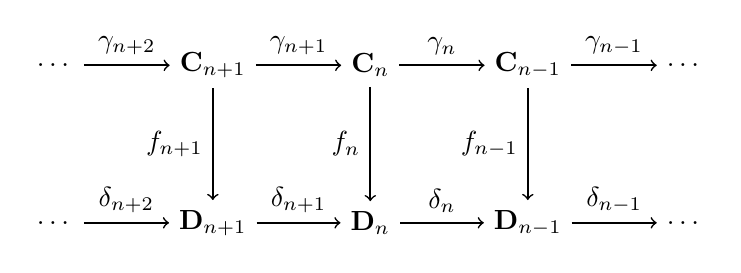
\begin{tikzpicture}[->,-latex, auto, every path/.style={->, semithick}, main node/.style={}]
\node	[main node]		(1) at (0,0)		{\dots};
\node	[main node]		(2) at (2,0)		{$\mathbf{C}_{n+1}$};
\node	[main node]		(3) at (4,0)		{$\mathbf{C}_{n}$};
\node [main node]		(4) at (6,0)		{$\mathbf{C}_{n-1}$};
\node [main node]		(5) at (8,0)		{$\dots$};
\node	[main node]		(6) at (0,-2)		{\dots};
\node	[main node]		(7) at (2,-2)		{$\mathbf{D}_{n+1}$};
\node	[main node]		(8) at (4,-2)		{$\mathbf{D}_{n}$};
\node [main node]		(9) at (6,-2)		{$\mathbf{D}_{n-1}$};
\node [main node]		(10) at (8,-2)		{\dots};

\draw (1) edge node [auto] {$\gamma_{n+2}$} (2);
\draw (2) edge node [auto] {$\gamma_{n+1}$} (3);
\draw (3) edge node [auto] {$\gamma_n$} (4);
\draw (4) edge node [auto] {$\gamma_{n-1}$} (5);
\draw (6) edge node [auto] {$\delta_{n+2}$} (7);
\draw (7) edge node [auto] {$\delta_{n+1}$} (8);
\draw (8) edge node [auto] {$\delta_n$} (9);
\draw (9) edge node [auto] {$\delta_{n-1}$} (10);
\draw (2) edge node [auto, swap] {$f_{n+1}$} (7);
\draw (3) edge node [auto, swap] {$f_n$} (8);
\draw (4) edge node [auto, swap] {$f_{n-1}$} (9);
\end{tikzpicture}
\end{equation*}
Note that there is an equivalent notion of a \emph{cochain map} of cochain complexes.
\end{mydef}

\begin{eg}
If we have the following diagram,
\begin{equation*}
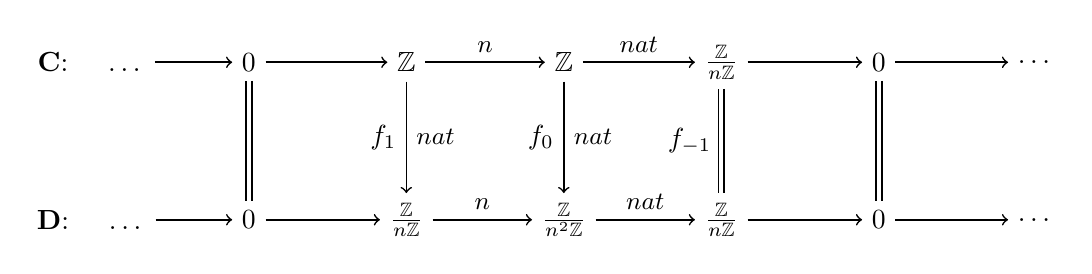
\begin{tikzpicture}[->,-latex, auto, main path/.style={->, semithick}, main node/.style={}]
\node	[main node]		(1) at (0,0)		{$\mathbf{C}$: \quad \dots};
\node	[main node]		(2) at (2,0)		{$0$};
\node	[main node]		(3) at (4,0)		{$\bb{Z}$};
\node [main node]		(4) at (6,0)		{$\bb{Z}$};
\node [main node]		(5) at (8,0)		{$\frac{\bb{Z}}{n\bb{Z}}$};
\node	[main node]		(11) at (10,0)	{$0$};
\node [main node] 		(12) at (12,0)	{\dots};
\node	[main node]		(6) at (0,-2)		{$\mathbf{D}$: \quad \dots};
\node	[main node]		(7) at (2,-2)		{$0$};
\node	[main node]		(8) at (4,-2)		{$\frac{\bb{Z}}{n\bb{Z}}$};
\node [main node]		(9) at (6,-2)		{$\frac{\bb{Z}}{n^2\bb{Z}}$};
\node [main node]		(10) at (8,-2)	{$\frac{\bb{Z}}{n\bb{Z}}$};
\node [main node]		(13) at (10,-2)	{$0$};
\node [main node]		(14) at (12,-2)	{\dots};

\draw (1) edge [main path] node [auto] {$$} (2);
\draw (2) edge [main path] node [auto] {$$} (3);
\draw (3) edge [main path] node [auto] {\small $n$} (4);
\draw (4) edge [main path] node [auto] {\small $nat$} (5);
\draw (5) edge [main path] (11);
\draw (11) edge [main path] (12);
\draw (6) edge [main path] node [auto] {$$} (7);
\draw (7) edge [main path] node [auto] {$$} (8);
\draw (8) edge [main path] node [auto] {\small $n$} (9);
\draw (9) edge [main path] node [auto] {\small $nat$} (10);
\draw (10) edge [main path] (13);
\draw (13) edge [main path] (14);
\draw (3) edge [main path] node [auto, swap] {$f_{1}$} node [auto] {\small $nat$} (8);
\draw (4) edge [main path] node [auto, swap] {$f_{0}$} node [auto] {\small $nat$} (9);
\draw (5) edge [-, semithick, double, double distance=1.5pt] node [auto, swap] {$f_{-1}$} (10);
\draw (11) edge [-, semithick, double, double distance=1.5pt] (13);
\draw (2) edge [-, semithick, double, double distance=1.5pt] (7);
\end{tikzpicture}
\end{equation*}
then we can see that our non trivial chain maps are, 
\begin{align*}
f_{1} &: \bb{Z} \to \frac{\bb{Z}}{n\bb{Z}}, \quad z \mapsto z+n\bb{Z},\\
f_0 &: \bb{Z} \to \frac{\bb{Z}}{n^2\bb{Z}}, \quad z \mapsto z+n^2\bb{Z}, \\
f_{1} &: \frac{\bb{Z}}{n\bb{Z}} \to \frac{\bb{Z}}{n\bb{Z}}, \quad z+n\bb{Z} \mapsto z+n\bb{Z}, 
\end{align*}
and they satisfy, 
\begin{equation*}
f_0(\gamma_1(z))=f_0(nz)=nz+n\bb{Z}=0\quad \& \quad \delta_1(f_1(z))=\delta_1(z+n\bb{Z})=nz+n\bb{Z}=0.
\end{equation*}
Simmilarly, we can see that the other chain maps make the diagram commute.
\end{eg}





















%%%%%%%%%%%%%%%%%%%%%%%%%%%%%%%%%%%%%%%%%%%%%%%%%%%%%
%%%%%%%%%%%%%%%%		EXACT SEQUENCES			%%%%%%%%%%%%%%%%%%%%
%%%%%%%%%%%%%%%%%%%%%%%%%%%%%%%%%%%%%%%%%%%%%%%%%%%%%

\section{Exact Sequences}

\begin{mydef}
A finite or infinite sequence of $R$-morphisms and left $R$-modules,
\begin{equation*}
\dots \xrightarrow{} L \xrightarrow{f}M \xrightarrow{g} N \xrightarrow{} \dots
\end{equation*}
is said to be \emph{exact} at $M$ if $imf=kerg$. A finite or infinite sequence of $R$-morphisms and left $R$-modules,
\begin{equation*}
\dots \xrightarrow{f_{n+2}} M_{n+1} \xrightarrow{f_{n+1}} M_n \xrightarrow{f_n} M_{n-1} \xrightarrow{f_{n-1}} \dots
\end{equation*}
is said to be an \emph{exact sequence} if it is exact at every $M_i$, i.e. $imf_i=kerf_{i+1}$. 
\end{mydef}

\begin{eg}
The finite sequence,
\begin{equation*}
0\xrightarrow{}k\xrightarrow{f}k^2\xrightarrow{g}k^2\xrightarrow{h}k^2\xrightarrow{}0,
\end{equation*}
where $f(x)=(x,0)$, $g(x, y)=(0,y)$, and $h(x,y)=(x,0)$ is an exact sequence since $im(f)=\{(x,0):x\in k\}=ker(g)$ and $im(g)=\{(0,y):u\in k\}=ker(h)$. 
However, if we instead consider the finite sequence, 
\begin{equation*}
0\xrightarrow{}k\xrightarrow{f}k^2\xrightarrow{g}k^2\xrightarrow{h'}k^2\xrightarrow{}0,
\end{equation*}
where $f$ and $g$ are the same as above, but $h'(x,y)=(x,y)$. Obviously, once again we have that $im(f)=ker(g)$ and $im(g)=\{(0,y):y\in k\}$, however, $ker(h')=\{(0,0)\}$ and so $im(g)\neq ker(h')$. Hence this is not an exact sequence, because it is not exact everywhere.
\end{eg}


\begin{mydef}
A \emph{short exact sequence} is an exact sequence of the form,
\begin{equation*}
0\xrightarrow{}L\xrightarrow{f}M\xrightarrow{g}N\xrightarrow{}0.
\end{equation*}
This is also referred to as and \emph{extension of} $N$ \emph{by} $L$.
\end{mydef}

\begin{eg}
The sequence,
\begin{equation*}
0\xrightarrow{} k \xrightarrow{f} k^2 \xrightarrow{g} k \xrightarrow{} 0,
\end{equation*}
where $f(x)=(x,0)$ and $g(x,y)=y$ is a short exact sequence, since $im(f)=\{(x,0): x\in k\}=ker(g)$.
\end{eg}

\begin{eg}
Notice that the sequence, 
\begin{equation*}
0\xrightarrow{}\bb{Z}\xrightarrow[6]{f}\bb{Z}\xrightarrow{\eta}\frac{\bb{Z}}{3\bb{Z}}\xrightarrow{} 0,
\end{equation*}
has $ker(\eta)=\{z:z+s\bb{Z}=0\cong 3\bb{Z}$ and $im(f)=\{6z:z\in \bb{Z}\}\cong 6\bb{Z}$. Hence, as $6\bb{Z}\subsetneq 3\bb{Z}$, $im(f)\neq ker(\eta)$ and the sequence is not exact.
\end{eg}

Notice that you can obtain a chain complex from an exact sequence simply by deciding the degree of any term of the sequence. To consider the result when a chain complex is an exact sequence, the following is in response to Exercise 1.1.5 from \cite{Weibel}. (Note that the third condition has been omitted as we are not consider quasi-isomerism in this report.)

\begin{thm}
The following are equivalent for every chain complex $\mathbf{C}$:
\begin{enumerate}
\item $\mathbf{C}$ is an exact sequence, that is, exact at every $C_n$.
\item $\mathbf{C}$ is acyclic, that is, $H_n(\mathbf{C})=0$ for all $n$.
\end{enumerate}
\end{thm}
\begin{proof}
Suppose the chain complex, 
\begin{equation*}
\mathbf{C}:\qquad \dots \xrightarrow{} C_{n+1} \xrightarrow{\delta_{n+1}} C_n \xrightarrow{\delta_n} C_{n-1} \xrightarrow{\delta_{n-1}} \dots
\end{equation*}
is an exact sequence, so we have that $im(\delta_{n+1})=ker(\delta_n)$ for all $n$, i.e. $B_n(\mathbf{C})=Z_n(\mathbf{C})$ for all $n$. Hence, when we compute the homology of $\mathbf{C}$, we find that,
\begin{equation*}
H_n(\mathbf{C})=\frac{Zn(\mathbf{C})}{B_n(\mathbf{C})}=0 \quad \forall n.
\end{equation*}
Thus, $\mathbf{C}$ is acyclic.\\
Conversely, suppose $\mathbf{C}$ is acyclic, then we have that $H_n(\mathbf{C})=0$ for all n. Therefore, $\sfrac{Z_n(\mathbf{C})}{B_n(\mathbf{C})}=0$ for all n, by definition, but this is only possibly if either $Z_n(\mathbf{C})\subset B_n(\mathbf{C})$, which is impossible from Definition \ref{iminkerlem}, or $Z_n(\mathbf{C})=B_n(\mathbf{C})$. Thus, $ker(\delta_n)=im(\delta_{n+1})$ and so $\mathbf{C}$ is exact.
\end{proof}

\begin{rem}
The above theorem makes it clear that exact sequences can be thought of as acyclic chain complexes. By the same token, homology can be thought of as a chain complex's deviation from exactness.
\end{rem}

The folllowing is provided as an example in \cite{Schiff}, however, it was felt too useful as a method of constructing exact sequences to be simply an example and so is presented on this report as a lemma.

\begin{prop} \label{cokerseqprop}
The sequence,
\begin{equation*}
0 \xrightarrow{} ker(f) \xrightarrow{\iota} M \xrightarrow{f} N \xrightarrow{\eta} coker(f) \xrightarrow{} 0,
\end{equation*} 
where $\iota , \eta$ are the inclusion, and natural maps respectively, is exact. In addition the sequence, 
\begin{equation*}
0\xrightarrow{} ker(f) \xrightarrow{\iota} M \xrightarrow{\eta} \frac{M}{im(f)} \xrightarrow{} 0,
\end{equation*}
is a short exact sequence.
\end{prop}
\begin{proof}
It is clear here that we have $im(\iota)=ker(f)$ as $\iota$ is the inclusion map and since $coker(f)=\sfrac{N}{im(f)}$ we also have that $im(f)=ker(\eta)$. Hence the sequence is exact. The second result follows a similar argument.
\end{proof}

\begin{eg}
Consider the map $f:\bb{Z}^2 \to \bb{Z}$, $(x, y)\mapsto 2x$. Then $ker(f)=\{(0,y):y\in \bb{Z}\}\cong \bb{Z}$, and $im(f)=2\bb{Z}$ giving that $coker(f)=\frac{\bb{Z}}{2\bb{Z}}$. It follows from Lemma \ref{cokerseqprop} that the sequence, 
\begin{equation*}
0 \xrightarrow{} \bb{Z} \xrightarrow{\iota} \bb{Z}^2 \xrightarrow{f} \bb{Z} \xrightarrow{\eta} \frac{\bb{Z}}{2\bb{Z}} \xrightarrow{} 0,
\end{equation*}
is exact. In addition, the following is a short exact equation,
\begin{equation*}
0\xrightarrow{} \bb{Z} \xrightarrow{\iota} \bb{Z}^2 \xrightarrow{\eta} \frac{\bb{Z}}{2\bb{Z}} \xrightarrow{}0.
\end{equation*}
\end{eg}

Here are some simple properties of exact sequences as detailed by Rotman in Proposition 2.18 of \cite{Rotman}. Also included is the solution to Exercise 2.16 (ii) from \cite{Rotman}; it caught our attention as an interesting property, with such a simple proof, which shows the rigidity of the exactness condition.

\begin{prop} \label{exactpropertiesprop}
\begin{description}
\item[(i)] A sequence $0\xrightarrow{}L\xrightarrow{f}M$ is exact if and only if $f$ is injective.
\item[(ii)] A sequence $M\xrightarrow{g}N\xrightarrow{}0$ is exact if and only if $g$ is surjective.
\item[(iii)] A sequence $0\xrightarrow{}L\xrightarrow{h}M\xrightarrow{}0$ is exact if and only if $h$ is an isomorphism.
\item[(iv)] If $:L\xrightarrow{f} M \xrightarrow{g}N\xrightarrow{h}L'$ then $f$ is surjective if and only if $h$ is injective.
\end{description}
\end{prop}
\begin{proof}
\begin{description}
\item[(i)] As the image of $0\xrightarrow{}L$ is $\{0\}$, exactness gives $ker(f)=\{0\}$, and so $f$ is injective. Conversely, given some map $f:L\to M$, there is an exact sequence $ker(f)\xrightarrow{\iota}L\rightarrow{f}M$, where $\iota$ is the inclusion map, (see Proposition \ref{cokerseqprop}). If $f$ is injective, then $ker(f)=\{0\}$.
\item[(ii)] The kernel of $N\xrightarrow{}0$ is $N$, so the exactness gives $im(g)=N$, and so $g$ is surjective. Conversely, given $g:M\to N$, there is an exact sequence $M\xrightarrow{g}N\xrightarrow{\pi}coker(g)$, where $\pi$ is the natural map, (see Proposition \ref{cokerseqprop}). If $g$ is surjective, then $N=im(g)$ and $coker(g)=\{0\}$.
\item[(iii)] Part (i) shows that the sequence is exact at $L$ if and only if $h$ is injective, and part (ii) shows that the sequence is exact at $M$ if and only if $h$ is surjective. Therefore, the sequence is exact everywhere if and only if $h$ is an isomorphism.
\item[(iv)] Suppose $f$ is surjective, them $im(f)=M$, and exactness at $M$ gives $ker(g)=M$. Hence, $im(g)=\{0\}$, and exactness at $N$ gives $ker(h)=\{0\}$ and so $h$ is injective. The converse is similar.
\end{description}
\end{proof}

\begin{mydef}
Two short exact sequences,
\begin{equation*}
\mathbf{E}: \quad 0\xrightarrow{}L\xrightarrow{}M\xrightarrow{}N\xrightarrow{}0 \qquad \& \qquad \mathbf{E'}: \quad 0\xrightarrow{}L\xrightarrow{}M'\xrightarrow{}N\xrightarrow{}0 ,
\end{equation*}
are \emph{equivalent} if there is a map $\xi: M \to M'$ such that the diagram,
\begin{equation*}
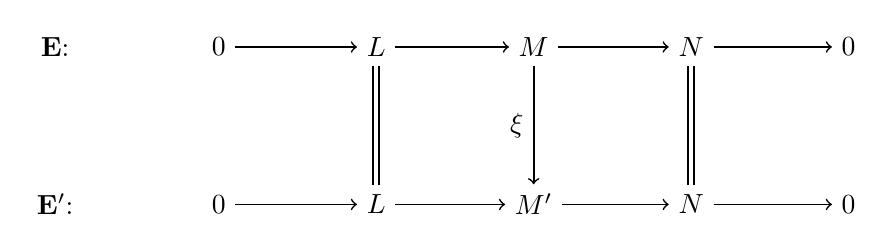
\begin{tikzpicture}[->,-latex, auto, main path/.style={->, semithick}, main node/.style={}]
\node	[main node]		(1) at (0,0)		{$\mathbf{E}$: \quad };
\node	[main node]		(2) at (2,0)		{$0$};
\node	[main node]		(3) at (4,0)		{$L$};
\node [main node]		(4) at (6,0)		{$M$};
\node [main node]		(5) at (8,0)		{$N$};
\node	[main node]		(11) at (10,0)	{$0$};

\node	[main node]		(6) at (0,-2)		{$\mathbf{E'}$: \quad};
\node	[main node]		(7) at (2,-2)		{$0$};
\node	[main node]		(8) at (4,-2)		{$L$};
\node [main node]		(9) at (6,-2)		{$M'$};
\node [main node]		(10) at (8,-2)	{$N$};
\node [main node]		(13) at (10,-2)	{$0$};

\draw (2) edge [main path] node [auto] {$$} (3);
\draw (3) edge [main path] node [auto] {$$} (4);
\draw (4) edge [main path] node [auto] {$$} (5);
\draw (5) edge [main path] (11);

\draw (7) edge [main path] node [auto] {$$} (8);
\draw (8) edge [main path] node [auto] {$$} (9);
\draw (9) edge [main path] node [auto] {$$} (10);
\draw (10) edge [main path] (13);

\draw (3) edge [-, semithick, double, double distance=1.5pt] (8);
\draw (4) edge [main path] node [auto, swap] {$\xi$} (9);
\draw (5) edge [-, semithick, double, double distance=1.5pt](10);
\end{tikzpicture}
\end{equation*}
commutes.\\
The equivalence classes of extensions of $N$ by $L$ will be represented as $e(N,L)$.
\end{mydef}

\begin{eg}
Consider the two short exact sequences, 
\begin{equation*}
\mathbf{E}: \quad 0\xrightarrow{}k\xrightarrow{f}k^2\xrightarrow{g}k\xrightarrow{}0  \quad \& \quad \mathbf{E'}: \quad 0\xrightarrow{}k\xrightarrow{f'}k^2\xrightarrow{g'}k\xrightarrow{}0 ,
\end{equation*}
where $f: x \mapsto (x, 0)$, $g: (x,y)\mapsto y$, $f':x \mapsto (0,x)$ and $g':(x,y)\mapsto x$. Then we can construct the diagram: 
\begin{equation*}
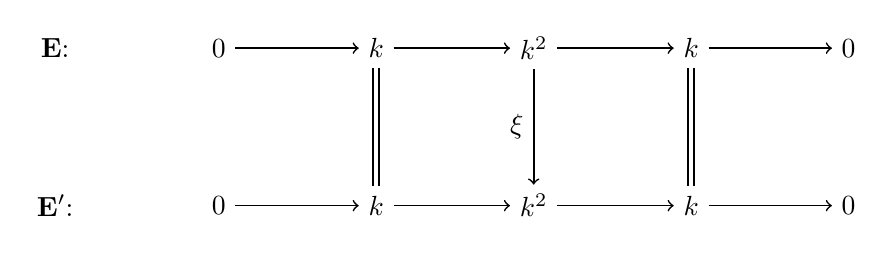
\begin{tikzpicture}[->,-latex, auto, main path/.style={->, semithick}, main node/.style={}]
\node	[main node]		(1) at (0,0)		{$\mathbf{E}$: \quad };
\node	[main node]		(2) at (2,0)		{$0$};
\node	[main node]		(3) at (4,0)		{$k$};
\node [main node]		(4) at (6,0)		{$k^2$};
\node [main node]		(5) at (8,0)		{$k$};
\node	[main node]		(11) at (10,0)	{$0$};

\node	[main node]		(6) at (0,-2)		{$\mathbf{E'}$: \quad};
\node	[main node]		(7) at (2,-2)		{$0$};
\node	[main node]		(8) at (4,-2)		{$k$};
\node [main node]		(9) at (6,-2)		{$k^2$};
\node [main node]		(10) at (8,-2)	{$k$};
\node [main node]		(13) at (10,-2)	{$0$};



\draw (2) edge [main path] node [auto] {$$} (3);
\draw (3) edge [main path] node [auto] {$$} (4);
\draw (4) edge [main path] node [auto] {$$} (5);
\draw (5) edge [main path] (11);


\draw (7) edge [main path] node [auto] {$$} (8);
\draw (8) edge [main path] node [auto] {$$} (9);
\draw (9) edge [main path] node [auto] {$$} (10);
\draw (10) edge [main path] (13);

\draw (3) edge [-, semithick, double, double distance=1.5pt] (8);
\draw (4) edge [main path] node [auto, swap] {$\xi$} (9);
\draw (5) edge [-, semithick, double, double distance=1.5pt](10);
\end{tikzpicture}
\end{equation*}
This diagram commutes when $\xi$ is the map $\xi: k^2 \to k^2$, $(x, y) \mapsto (y, x)$, hence these two short exact equations are equivalent.
\end{eg}

For a nonexample we turn to Exercise \uppercase\expandafter{\romannumeral 3} 1.1 in \cite{Stamm}.

\begin{eg}
Consider the two short exact sequences, 
\begin{equation*}
\mathbf{E}: \quad 0\xrightarrow{}\bb{Z}\xrightarrow{f}\bb{Z}\xrightarrow{g}\frac{\bb{Z}}{3\bb{Z}}\xrightarrow{}0  \quad \& \quad \mathbf{E'}: \quad 0\xrightarrow{}\bb{Z}\xrightarrow{f'}\bb{Z}\xrightarrow{g'}\frac{\bb{Z}}{3\bb{Z}}\xrightarrow{}0 ,
\end{equation*}
where $f, f': x\mapsto 3x$, $g: x \mapsto x(\text{mod }3)$ and $g':x\mapsto 2x(\text{mod }3)$. Then we can construct the diagram: 
\begin{equation*}
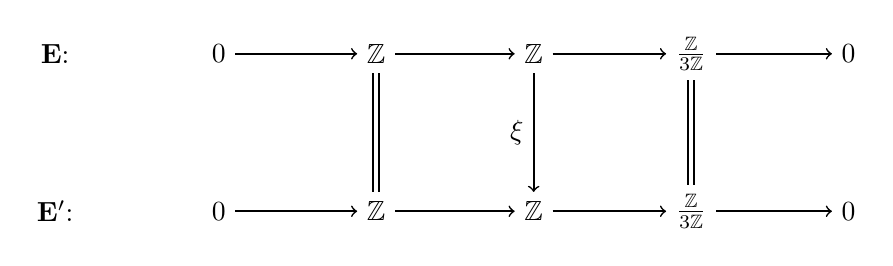
\begin{tikzpicture}[->,-latex, auto, main path/.style={->, semithick}, main node/.style={}]
\node	[main node]		(1) at (0,0)		{$\mathbf{E}$: \quad };
\node	[main node]		(2) at (2,0)		{$0$};
\node	[main node]		(3) at (4,0)		{$\bb{Z}$};
\node [main node]		(4) at (6,0)		{$\bb{Z}$};
\node [main node]		(5) at (8,0)		{$\frac{\bb{Z}}{3\bb{Z}}$};
\node	[main node]		(11) at (10,0)	{$0$};

\node	[main node]		(6) at (0,-2)		{$\mathbf{E'}$: \quad};
\node	[main node]		(7) at (2,-2)		{$0$};
\node	[main node]		(8) at (4,-2)		{$\bb{Z}$};
\node [main node]		(9) at (6,-2)		{$\bb{Z}$};
\node [main node]		(10) at (8,-2)	{$\frac{\bb{Z}}{3\bb{Z}}$};
\node [main node]		(13) at (10,-2)	{$0$};

\draw (2) edge [main path] node [auto] {$$} (3);
\draw (3) edge [main path] node [auto] {$$} (4);
\draw (4) edge [main path] node [auto] {$$} (5);
\draw (5) edge [main path] (11);


\draw (7) edge [main path] node [auto] {$$} (8);
\draw (8) edge [main path] node [auto] {$$} (9);
\draw (9) edge [main path] node [auto] {$$} (10);
\draw (10) edge [main path] (13);

\draw (3) edge [-, semithick, double, double distance=1.5pt] (8);
\draw (4) edge [main path] node [auto, swap] {$\xi$} (9);
\draw (5) edge [-, semithick, double, double distance=1.5pt](10);
\end{tikzpicture}
\end{equation*}
Assume $\mathbf{E}$ and $\mathbf{E'}$ are equivalent, so we there must exist some $\xi$ such that the diagram commutes. The second square in the diagram will commute if and only if $\xi=id_{\bb{Z}}$, since $f=f'$, however, this then means the third square will never commute, as $g\neq g'$. Thus no such $\xi$ exists and the two short exact sequences are not equivalent.
\end{eg}

For the discussion of split exact sequences, this report will first follow \cite{Schiff} in defining a section and refraction and then use Schiffler's Proposition 1.8 to prove that the conditions in Definition 1.23 in \cite{CB1} are equivalent. This will obtain us the Splitting Lemma. However, the proof of Proposition 1.8 will be ommitted as it is 

\begin{mydef} \label{secretdef}
\begin{itemize}
\item A map $f: L \to M$ is called a \emph{section} if there exists a map $h: M \to L$ such that $hf=id_L$.
\item A map $g:M\to N$ is called a \emph{retraction} if there exists a map $h: N \to M$ such that $gh=id_N$.
\end{itemize}
\end{mydef}

\begin{mydef}
A short exact sequence,
\begin{equation*}
0\xrightarrow{}L\xrightarrow{f} M \xrightarrow{g} N \xrightarrow{} 0,
\end{equation*}
is said to be \emph{split} if $f$ is a section.
\end{mydef}

\begin{lem} \label{splittinglem} (Splitting Lemma)
If the short exact sequence, 
\begin{equation*}
0\xrightarrow{}L\xrightarrow{f} M \xrightarrow{g} N \xrightarrow{} 0,
\end{equation*}
is split then the following equivalent conditions hold:
\begin{description}
\item [(i)] $f$ is a section.
\item [(ii)] $g$ is a retraction.
\item [(iii)] $im(f)$ is a direct summand of $M$.
\end{description}
\end{lem}
\begin{proof}
Proof omitted. See Proposition 1.8 in \cite{Schiff} and the proof given on \cite{Splittinglem}.
\end{proof}

\begin{eg}
The short exact sequence, 
\begin{equation*}
0 \xrightarrow{}\bb{Z} \xrightarrow{f} \bb{Z}^2 \xrightarrow{g} \bb{Z} \xrightarrow{} 0,
\end{equation*}
where $f: x \mapsto (x, 0)$ and $g: (x, y) \mapsto y$, splits. Then
\begin{description}
\item [(i)] $f$ is a section as the map $h:\bb{Z}^2 \to \bb{Z}$, $(x, y) \mapsto x$ satifies $hf=id_{\bb{Z}}$.
\item [(ii)] $g$ is a retraction as the map $h': \bb{Z} \to \bb{Z}^2$, $y \mapsto (x, y)$ satifies $gh=id_{\bb{Z}}$.
\item [(iii)] $im(f) \cong \bb{Z}$ is a direct summand of $\bb{Z}^2 \cong \bb{Z}\oplus \bb{Z}$.
\end{description}
\end{eg}

Rather than provide the following result as a proposition and prove it directly as Rotman does in \cite{Rotman}, it will be given as a corollary of the splitting lemma as in \cite{Schiff}.

\begin{cor} \label{MLNcor}
If the sequence,
\begin{equation*}
0\xrightarrow{}L\xrightarrow{f} M \xrightarrow{g} N \xrightarrow{} 0,
\end{equation*}
is split exact, then
\begin{equation*}
M \cong L \oplus N.
\end{equation*}
\end{cor}
\begin{proof}
Since $f$ is injective as the seqence is short exact, we have $L \cong im(f) \cong ker(g)$. The since $g$ is surjective as the sequence is short exact, the first isomorphism theorem implies $N \cong \sfrac{M}{ker(g)}$. Then Lemma \ref{splittinglem} gives $M$  is a direct summand of $im(f)$, hence, $M\cong L \oplus N$.
\end{proof}

\begin{eg}
Notice that in the previous example $\bb{Z} \cong im(f)\cong ker(g) $ and $\bb{Z} \cong \sfrac{\bb{Z}^2}{ker(g)}\cong \bb{Z}$. Hence, $\bb{Z}^2 \cong \bb{Z} \oplus \bb{Z}$, as expected.
\end{eg}

\begin{lem} \label{splitequivlem}
If any two extensions of $N$ by $L$ are split, then they are equivalent.
\end{lem}
\begin{proof}
Let,
\begin{equation*}
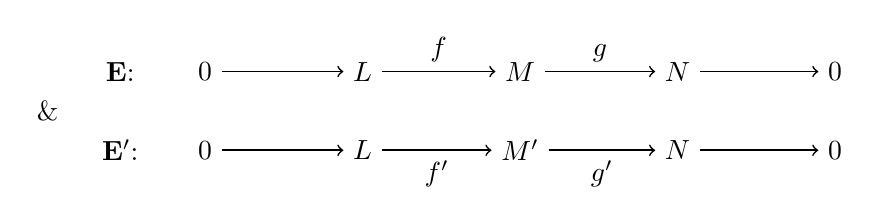
\begin{tikzpicture}[->,-latex, auto, main path/.style={->, semithick}, main node/.style={}]
\node	[main node]		(1) at (1,0)		{$\mathbf{E}$: \quad };
\node	[main node]		(2) at (2,0)		{$0$};
\node	[main node]		(3) at (4,0)		{$L$};
\node [main node]		(4) at (6,0)		{$M$};
\node [main node]		(5) at (8,0)		{$N$};
\node	[main node]		(11) at (10,0)	{$0$};

\node [main node] 		(12) at (0,-0.5)	{\&};
\node	[main node]		(6) at (1,-1)		{$\mathbf{E'}$: \quad};
\node	[main node]		(7) at (2,-1)		{$0$};
\node	[main node]		(8) at (4,-1)		{$L$};
\node [main node]		(9) at (6,-1)		{$M'$};
\node [main node]		(10) at (8,-1)	{$N$};
\node [main node]		(13) at (10,-1)	{$0$};

\draw (2) edge [main path] node [auto] {$$} (3);
\draw (3) edge [main path] node [auto] {$f$} (4);
\draw (4) edge [main path] node [auto] {$g$} (5);
\draw (5) edge [main path] (11);

\draw (7) edge [main path] node [auto] {$$} (8);
\draw (8) edge [main path] node [auto, swap] {$f'$} (9);
\draw (9) edge [main path] node [auto, swap] {$g'$} (10);
\draw (10) edge [main path] (13);
\end{tikzpicture}
\end{equation*}
 be two split extensions of $N$ by $L$. Then Corollary \ref{MLNcor} gives $M \cong L\oplus N$ and $M'\cong L \oplus N$ and so there exists some isomorphism $M \cong M'$. 
\end{proof}

\begin{rem}
Notice also that if $\mathbf{E}, \mathbf{E'}$ are equivalent extensions and one is split, then the other is also split.
\end{rem}
\begin{proof}
As the extensions are equivalent we have the commutative diagram,
\begin{equation*}
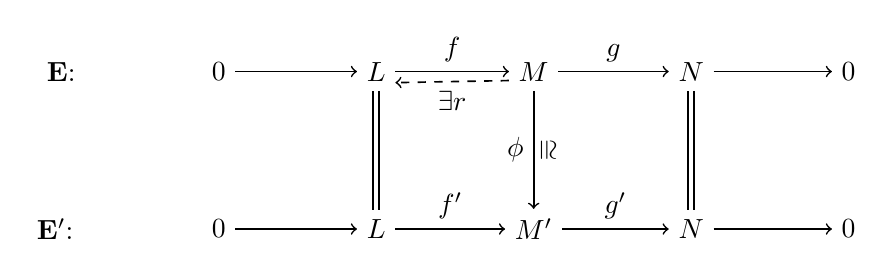
\begin{tikzpicture}[->,-latex, auto, main path/.style={->, semithick}, main node/.style={}]
\node	[main node]		(1) at (0,0)		{$\mathbf{E}$:};
\node	[main node]		(2) at (2,0)		{$0$};
\node	[main node]		(3) at (4,0)		{$L$};
\node [main node]		(4) at (6,0)		{$M$};
\node [main node]		(5) at (8,0)		{$N$};
\node	[main node]		(11) at (10,0)	{$0$};

\node	[main node]		(6) at (0,-2)		{$\mathbf{E'}$: \quad};
\node	[main node]		(7) at (2,-2)		{$0$};
\node	[main node]		(8) at (4,-2)		{$L$};
\node [main node]		(9) at (6,-2)		{$M'$};
\node [main node]		(10) at (8,-2)	{$N$};
\node [main node]		(13) at (10,-2)	{$0$};

\draw (2) edge [main path] node [auto] {$$} (3);
\path (3.0) edge [main path] node [auto] {$f$} (4.180);
\path (4.200) edge [dashed, ->, semithick] node [auto] {$\exists r$} (3.330);
\draw (4) edge [main path] node [auto] {$g$} (5);
\draw (5) edge [main path] (11);


\draw (7) edge [main path] node [auto] {$$} (8);
\draw (8) edge [main path] node [auto] {$f'$} (9);
\draw (9) edge [main path] node [auto] {$g'$} (10);
\draw (10) edge [main path] (13);

\draw (3) edge [-, semithick, double, double distance=1.5pt] (8);
\draw (4) edge [main path] node [above,sloped,inner sep=1pt] {$\cong$} node [auto, swap] {$\phi$} (9);
\draw (5) edge [-, semithick, double, double distance=1.5pt](10);
\end{tikzpicture}
\end{equation*}
As $\mathbf{E}$ splits, $f$ must be a secton and so there exists a map $r: M \to L$ such that $rf=id_L$. Then if $m'\in M'$ it can be mapped to some $\phi^{-1}(m')=m$ as $\phi$ is an isomorphism by equivalence, and so has an inverse. Hence $f'$ is a sections as there is the map, $r':M' \to L$, $m' \mapsto r(\phi^{-1}(m'))$. Thus $\mathbf{E'}$ is split.
\end{proof}

\begin{mydef} \label{pushoutdef}
Given a short exact seqence,
\begin{equation*}
\mathbf{E}: \qquad 0\xrightarrow{}L\xrightarrow{f} M \xrightarrow{g} N \xrightarrow{} 0,
\end{equation*}
and a map $\theta : L \to L'$ then the short exact sequence, 
\begin{equation*}
\mathbf{E'}: \qquad 0\xrightarrow{} L' \xrightarrow{f'} M' \xrightarrow{g'} N \xrightarrow{}0,
\end{equation*}
fitting into the commutative diagram
\begin{equation*}
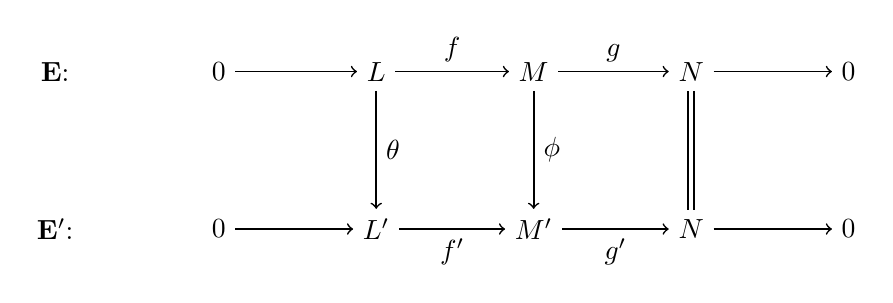
\begin{tikzpicture}[->,-latex, auto, main path/.style={->, semithick}, main node/.style={}]
\node	[main node]		(1) at (0,0)		{$\mathbf{E}$: \quad };
\node	[main node]		(2) at (2,0)		{$0$};
\node	[main node]		(3) at (4,0)		{$L$};
\node [main node]		(4) at (6,0)		{$M$};
\node [main node]		(5) at (8,0)		{$N$};
\node	[main node]		(11) at (10,0)	{$0$};

\node	[main node]		(6) at (0,-2)		{$\mathbf{E'}$: \quad};
\node	[main node]		(7) at (2,-2)		{$0$};
\node	[main node]		(8) at (4,-2)		{$L'$};
\node [main node]		(9) at (6,-2)		{$M'$};
\node [main node]		(10) at (8,-2)	{$N$};
\node [main node]		(13) at (10,-2)	{$0$};

\draw (2) edge [main path] node [auto] {$$} (3);
\draw (3) edge [main path] node [auto] {$f$} (4);
\draw (4) edge [main path] node [auto] {$g$} (5);
\draw (5) edge [main path] (11);

\draw (7) edge [main path] node [auto] {$$} (8);
\draw (8) edge [main path] node [auto, swap] {$f'$} (9);
\draw (9) edge [main path] node [auto, swap] {$g'$} (10);
\draw (10) edge [main path] (13);

\draw (3) edge [main path] node [auto] {$\theta$} (8);
\draw (4) edge [main path] node [auto] {$\phi$} (9);
\draw (5) edge [-, semithick, double, double distance=1.5pt](10);
\end{tikzpicture}
\end{equation*}
is defined to be the \emph{pushout of $\mathbf{E}$ along $\theta$}.
\end{mydef}

\begin{prop} \label{pushoutprop}
Let $\mathbf{E}$, $\mathbf{E'}$ and $\theta: L \to L'$ be defined as above in Definition \ref{pushoutdef}. Then the pushout of $\mathbf{E}$ along $\theta$ exists and is unique up to equivalence.
\end{prop}
\begin{proof}
Existence: Firstly, set
\begin{equation*}
M'=\frac{(L'\oplus M)}{\{(\theta(l), -f(l)): l\in L\}},
\end{equation*}
and let the maps be $f': l'\mapsto \overline{(l',0)}$, $g': \overline{(l',m)}\mapsto g(m)$ and $\phi: m \mapsto \overline{(0,m)}$, where $\overline{(l',m)}$ denotes the class of $(l', m) \in L'\oplus M$ in $M'$. The diagram is then commutative as $\phi(f(l))=\overline{(0,f(l))}=\overline{(0,0)}=\overline{(\theta(l),0)}=f'(\theta(l))$ for an $l\in L$ and $id_N(g(m))=g(m)=g'(\theta(m))$ for any $m\in M$. The pushout is exact as $im(f')=\{\overline{(l',0)}:l'\in L'\}=ker(g')$.\\
Uniqueness: The sequence
\begin{equation*}
\mathbf{\xi'} \qquad 0\xrightarrow{}L \xrightarrow{\begin{psmallmatrix}\theta \\ -f \end{psmallmatrix}} L'\oplus M \xrightarrow{\begin{psmallmatrix} f' & \phi \end{psmallmatrix}} M' \xrightarrow{} 0,
\end{equation*}
is exact as $im(\begin{psmallmatrix}\theta \\ -f \end{psmallmatrix})=\{\begin{psmallmatrix}\theta(l) \\ -f(l) \end{psmallmatrix}: l \in L\}=ker(\begin{psmallmatrix} f' & \phi \end{psmallmatrix})$. Exactness then implies that $\begin{psmallmatrix} f' & \phi \end{psmallmatrix}$ is surjective and so by the first isomorphism theorem (see proof of Corollary \ref{MLNcor}) we have,
\begin{equation*}
M' \cong \frac{L'\oplus M}{ker(\begin{psmallmatrix} f' & \phi \end{psmallmatrix})} \cong \frac{L'\oplus M}{\{(\theta(l), -f(l)): l\in L\}}.
\end{equation*}
This gives equivalence between $\mathbf{E'}$ and $\mathbf{E''}$.
\end{proof}

\begin{eg}
Consider the short exact sequence,
\begin{equation*}
\mathbf{E}: \qquad 0\xrightarrow{} \bb{Z} \xrightarrow[f]{n} \bb{Z}\xrightarrow[g]{nat}\frac{\bb{Z}}{n\bb{Z}} \xrightarrow{} 0,
\end{equation*}
and the $\bb{Z}$-module map $\theta: \bb{Z} \to \sfrac{\bb{Z}}{n\bb{Z}}$ is the natural one. Now we can use Proposition \ref{pushoutprop} to construct the pushout of $\mathbf{E}$ along $\theta$.\\
Firstly, construct the commutative diagram,
\begin{equation*}
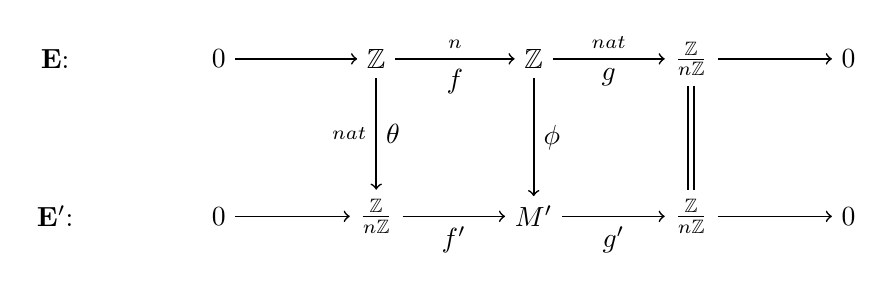
\begin{tikzpicture}[->,-latex, auto, main path/.style={->, semithick}, main node/.style={}]
\node	[main node]		(1) at (0,0)		{$\mathbf{E}$: \quad };
\node	[main node]		(2) at (2,0)		{$0$};
\node	[main node]		(3) at (4,0)		{$\bb{Z}$};
\node [main node]		(4) at (6,0)		{$\bb{Z}$};
\node [main node]		(5) at (8,0)		{$\frac{\bb{Z}}{n\bb{Z}}$};
\node	[main node]		(11) at (10,0)	{$0$};

\node	[main node]		(6) at (0,-2)		{$\mathbf{E'}$: \quad};
\node	[main node]		(7) at (2,-2)		{$0$};
\node	[main node]		(8) at (4,-2)		{$\frac{\bb{Z}}{n\bb{Z}}$};
\node [main node]		(9) at (6,-2)		{$M'$};
\node [main node]		(10) at (8,-2)	{$\frac{\bb{Z}}{n\bb{Z}}$};
\node [main node]		(13) at (10,-2)	{$0$};

\draw (2) edge [main path] node [auto] {$$} (3);
\draw (3) edge [main path] node [auto] {$\scriptstyle{n}$} node [auto, swap] {$f$} (4);
\draw (4) edge [main path] node [auto] {$\scriptstyle{nat}$} node [auto, swap] {$g$} (5);
\draw (5) edge [main path] (11);

\draw (7) edge [main path] node [auto] {$$} (8);
\draw (8) edge [main path] node [auto, swap] {$f'$} (9);
\draw (9) edge [main path] node [auto, swap] {$g'$} (10);
\draw (10) edge [main path] (13);

\draw (3) edge [main path] node [auto] {$\theta$} node [auto, swap] {$\scriptstyle{nat}$} (8);
\draw (4) edge [main path] node [auto] {$\phi$} (9);
\draw (5) edge [-, semithick, double, double distance=1.5pt](10);
\end{tikzpicture}
\end{equation*}
and now we want to find $M'$. As $\theta: x \mapsto x+n\bb{Z}$ and $f: x \mapsto nx$, we have,
\begin{equation*}
M'=\frac{\frac{\bb{Z}}{n\bb{Z}}\oplus\bb{Z}}{\{(x+n\bb{Z}, -nx):x \in \bb{Z}\}},
\end{equation*}
and we can set $f': \sfrac{\bb{Z}}{n\bb{Z}} \to M'$, $x+n\bb{Z} \mapsto \overline{(x+n\bb{Z},0)}$, $g': M' \to \sfrac{\bb{Z}}{n\bb{Z}}$, $\overline{(x+n\bb{Z}, y)} \mapsto y+n\bb{Z}$, and $\phi: \bb{Z} \to M'$, $x \mapsto \overline{(0,x)}$. It is clear that this makes the above diagram commutative and gives $\mathbf{E'}$ exact. Furthermore, the map $\phi$ is onto as,
\begin{align*}
M'\ni\overline{(x+n\bb{Z}, y)}&=\overline{(x+n\bb{Z}, -nx)} + \overline{(o, y+na)},\\
&=\overline{(0, y+nx)} \in im(\phi).
\end{align*}
We can also see that, 
\begin{align*}
ker(\phi)&= \{y\in \bb{Z}: \overline{(0, y)}=0\},\\
&=\{y\in \bb{Z}: \overline{(0, y)} \text{ is of the form } \overline{(x+n\bb{Z}, -nx)}\},\\
&=\{y\in \bb{Z}: n|y\text{, }x=\frac{-b}{n}\text{ and } x+n\bb{Z}=0\},\\
&=\{y\in \bb{Z}: n^2|y\}\cong n^2\bb{Z},
\end{align*}
and then the First Isomorphism Theorem gives, 
\begin{equation*}
M'\cong \frac{\bb{Z}}{ker(\phi)}\cong \frac{\bb{Z}}{n^2\bb{Z}}.
\end{equation*}
Hence, the pushout of $\mathbf{E}$ along $\theta$ is,
\begin{equation*}
\mathbf{E'}: \qquad 0\xrightarrow{} \frac{\bb{Z}}{n\bb{Z}} \xrightarrow{f'} \frac{\bb{Z}}{n^2\bb{Z}}\xrightarrow{g'} \frac{\bb{Z}}{n\bb{Z}} \xrightarrow{} 0,
\end{equation*}
with the maps $f', g'$ defined as above.
\end{eg}

\begin{mydef} \label{pullbackdef}
Given a short exact seqence,
\begin{equation*}
\mathbf{E}: \qquad 0\xrightarrow{}L\xrightarrow{f} M \xrightarrow{g} N \xrightarrow{} 0,
\end{equation*}
and a map $\psi: N''\to N$ then the short exact sequence, 
\begin{equation*}
\mathbf{E''}: \qquad 0\xrightarrow{} L \xrightarrow{f''} M'' \xrightarrow{g''} N'' \xrightarrow{}0,
\end{equation*}
fitting into the commutative diagram
\begin{equation*}
\begin{tikzpicture}[->,-latex, auto, main path/.style={->, semithick}, main node/.style={}]
\node	[main node]		(1) at (0,0)		{$\mathbf{E''}$: \quad };
\node	[main node]		(2) at (2,0)		{$0$};
\node	[main node]		(3) at (4,0)		{$L$};
\node [main node]		(4) at (6,0)		{$M''$};
\node [main node]		(5) at (8,0)		{$N''$};
\node	[main node]		(11) at (10,0)	{$0$};

\node	[main node]		(6) at (0,-2)		{$\mathbf{E}$: \quad};
\node	[main node]		(7) at (2,-2)		{$0$};
\node	[main node]		(8) at (4,-2)		{$L$};
\node [main node]		(9) at (6,-2)		{$M$};
\node [main node]		(10) at (8,-2)	{$N$};
\node [main node]		(13) at (10,-2)	{$0$};

\draw (2) edge [main path] node [auto] {$$} (3);
\draw (3) edge [main path] node [auto] {$f''$} (4);
\draw (4) edge [main path] node [auto] {$g''$} (5);
\draw (5) edge [main path] (11);

\draw (7) edge [main path] node [auto] {$$} (8);
\draw (8) edge [main path] node [auto, swap] {$f$} (9);
\draw (9) edge [main path] node [auto, swap] {$g$} (10);
\draw (10) edge [main path] (13);

\draw (3) edge [-, semithick, double, double distance=1.5pt] (8);
\draw (4) edge [main path] node [auto] {$\phi'$} (9);
\draw (5) edge[main path] node [auto] {$\psi$} (10);
\end{tikzpicture}
\end{equation*}
is defined to be the \emph{pullback} of $\mathbf{E}$ along $\psi$.
\end{mydef}

\begin{prop} \label{pullbackprop}
Let $\mathbf{E}$, $\mathbf{E''}$ and $\psi: N''\to N$ be defined as above in Definition \ref{pullbackdef}. Then the pullback of $\mathbf{E}$ along $\psi$ exists and is unique up to equivalence.
\end{prop}
\begin{proof}
Existence: Firstly, set
\begin{equation*}
M''=\{(m,n'')\in M\oplus N'': g(m)=\psi(n'')\},
\end{equation*}
and let the maps be $f'': L \to M''$, $l\mapsto (f(l),0)$ (if $g(f(l))=\psi(0)$, $0$ otherwise), $g'': M'' \to N''$, $(m, n'') \mapsto n''$, and $\phi': M'' \to M$, $(m, n'') \mapsto m$. The diagram is then commutative by diagram chasing and the pullback is exact as $im(f)=\{(f(l),0):l\in L\text{ and } g(f(l))=\psi(0)\}=\{(m, 0): m \in M\text{ and }g(m)=\psi(0)\}=ker(g'')$. 
Uniqueness: Consider the commutative diagram of short exact sequences,
\begin{equation*}
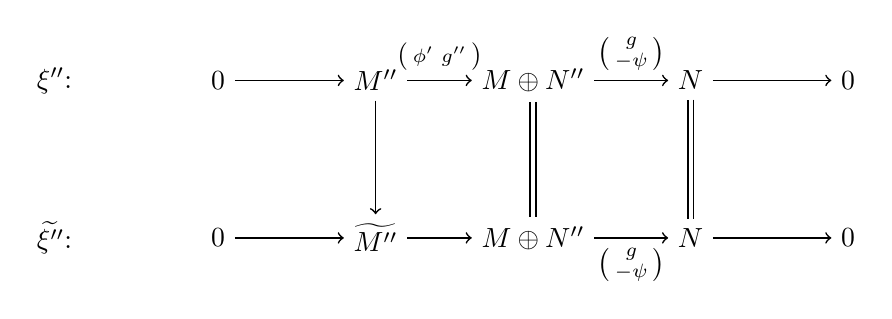
\begin{tikzpicture}[->,-latex, auto, main path/.style={->, semithick}, main node/.style={}]
\node	[main node]		(1) at (0,0)		{$\mathbf{\xi''}$: \quad };
\node	[main node]		(2) at (2,0)		{$0$};
\node	[main node]		(3) at (4,0)		{$M''$};
\node [main node]		(4) at (6,0)		{$M\oplus N''$};
\node [main node]		(5) at (8,0)		{$N$};
\node	[main node]		(11) at (10,0)	{$0$};

\node	[main node]		(6) at (0,-2)		{$\widetilde{\mathbf{\xi''}}$: \quad};
\node	[main node]		(7) at (2,-2)		{$0$};
\node	[main node]		(8) at (4,-2)		{$\widetilde{M''}$};
\node [main node]		(9) at (6,-2)		{$M\oplus N''$};
\node [main node]		(10) at (8,-2)	{$N$};
\node [main node]		(13) at (10,-2)	{$0$};

\draw (2) edge [main path] node [auto] {$$} (3);
\draw (3) edge [main path] node [auto] {$\begin{psmallmatrix}\phi' & g''\end{psmallmatrix}$} (4);
\draw (4) edge [main path] node [auto] {$\begin{psmallmatrix}g \\ -\psi \end{psmallmatrix}$} (5);
\draw (5) edge [main path] (11);

\draw (7) edge [main path] node [auto] {$$} (8);
\draw (8) edge [main path] node [auto, swap] {$$} (9);
\draw (9) edge [main path] node [auto, swap] {$\begin{psmallmatrix}g \\ -\psi \end{psmallmatrix}$} (10);
\draw (10) edge [main path] (13);

\draw (3) edge [main path] node [auto] {$$} (8);
\draw (4) edge [-, semithick, double, double distance=1.5pt] (9);
\draw (5) edge [-, semithick, double, double distance=1.5pt](10);
\end{tikzpicture}
\end{equation*}
where $M''$ and $\widetilde{M''}$ are from two pullbacks, $\mathbf{E''}$ and $\widetilde{\mathbf{E''}}$, of $\mathbf{E}$ along $\psi$. By diagram chasing we can see that there is in fact an isomorphism between $M''$ and $\widetilde{M''}$ and so $\mathbf{E''}$ and $\widetilde{\mathbf{E''}}$ are equivalent as short exact sequences.
\end{proof}

\begin{eg}
Consider the short exact sequence, 
\begin{equation*}
\mathbf{E}: \qquad 0\xrightarrow{} \bb{Z} \xrightarrow[f]{n} \bb{Z}\xrightarrow[g]{nat}\frac{\bb{Z}}{n\bb{Z}} \xrightarrow{} 0,
\end{equation*}
and the $\bb{Z}$-module map $\psi: \bb{Z} \to \sfrac{\bb{Z}}{n\bb{Z}}$ is the natural one. Now we can use Proposition \ref{pullbackprop} to construct the pullback of $\mathbf{E}$ along $\psi$.\\
Firstly, construct the commutative diagram,
\begin{equation*}
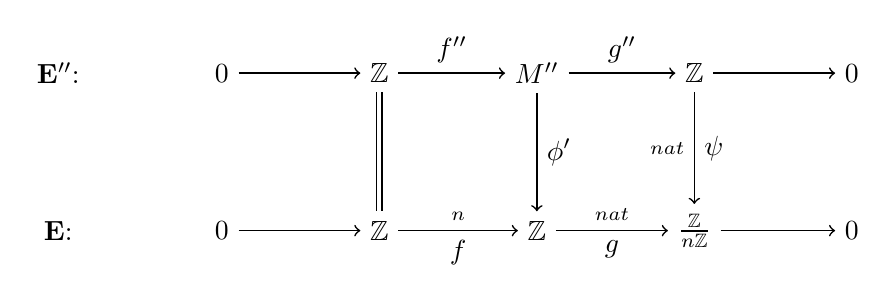
\begin{tikzpicture}[->,-latex, auto, main path/.style={->, semithick}, main node/.style={}]
\node	[main node]		(1) at (0,0)		{$\mathbf{E''}$: \quad };
\node	[main node]		(2) at (2,0)		{$0$};
\node	[main node]		(3) at (4,0)		{$\bb{Z}$};
\node [main node]		(4) at (6,0)		{$M''$};
\node [main node]		(5) at (8,0)		{$\bb{Z}$};
\node	[main node]		(11) at (10,0)	{$0$};

\node	[main node]		(6) at (0,-2)		{$\mathbf{E}$: \quad};
\node	[main node]		(7) at (2,-2)		{$0$};
\node	[main node]		(8) at (4,-2)		{$\bb{Z}$};
\node [main node]		(9) at (6,-2)		{$\bb{Z}$};
\node [main node]		(10) at (8,-2)	{$\frac{\bb{Z}}{n\bb{Z}}$};
\node [main node]		(13) at (10,-2)	{$0$};

\draw (2) edge [main path] node [auto] {$$} (3);
\draw (3) edge [main path]node [auto] {$f''$} (4);
\draw (4) edge [main path] node [auto] {$g''$} (5);
\draw (5) edge [main path] (11);

\draw (7) edge [main path] node [auto] {$$} (8);
\draw (8) edge [main path]  node [auto] {$\scriptstyle{n}$} node [auto, swap] {$f$} (9);
\draw (9) edge [main path] node [auto] {$\scriptstyle{nat}$}  node [auto, swap] {$g$} (10);
\draw (10) edge [main path] (13);

\draw (3) edge  [-, semithick, double, double distance=1.5pt](8);
\draw (4) edge [main path] node [auto] {$\phi'$} (9);
\draw (5) edge [main path] node [auto] {$\psi$} node [auto, swap] {$\scriptstyle{nat}$} (10);
\end{tikzpicture}
\end{equation*}
and now to find $M''$. As both $\psi, g: x \mapsto x+n\bb{Z}$, we have,
\begin{align*}
M''&=\{(x,y) \in \bb{Z} \oplus \bb{Z} : x+n\bb{Z}=y+n\bb{Z}\}, \\
&=\{(x, y) \in \bb{Z} \oplus \bb{Z}: n\divides x-y\}, \\
&\cong \bb{Z}\oplus\bb{Z},\text{ by considering the map } (a,b)\mapsto (a, a+nb),\\
&\cong \bb{Z}^2,
\end{align*}
and we can set $f'': \bb{Z} \to M''$, $x \mapsto \overline{(nx, 0)}$, $g'': M'' \to \bb{Z}$, $\overline{(x, y)} \mapsto y$ and $\phi': M'' \to \bb{Z}$, $\overline(x, y) \mapsto m$. It is clear that this makes the diagram commutative and gives $\mathbf{E''}$ exact. Hence, the pullback of $\mathbf{E}$ along $\psi$ is,
\begin{equation*}
\mathbf{E''}:\quad 0\xrightarrow{}\bb{Z} \xrightarrow{f''} \bb{Z}^2 \xrightarrow{g''} \bb{Z} \xrightarrow{}0,
\end{equation*}
with the maps $f'',g''$ defined as above.
\end{eg}

Now this report will start to consider the results possible by considering exact sequences of ....\\
%FILL THIS IN 
% Put in Weibel Exercise 1.3.1
% Add fives lemma??
The following theorem is from \cite{CB1} and the proof that the connecting map exists and is well defined taken from \cite{CB1} and the proof that the sequence induced by this map is exact from \cite{Weibel}. Both proofs were adapted to use the notation used in this report and some more explanation given when we felt it was necessary.

\begin{thm} (Long Exact Sequence) \label{longexactseqthm} \\
Let $0\xrightarrow{}\mathbf{C} \xrightarrow{f} \mathbf{D} \xrightarrow{g} \mathbf{E} \xrightarrow{}0$ be a short exact sequence of chain complexes, meaning that $f$ and $g$ are chain maps and for each $n$ the maps
\begin{equation*}
0 \xrightarrow{} C_n \xrightarrow{f_n} D_n \xrightarrow{g_n} E_n \xrightarrow{} 0,
\end{equation*}
form a short exact sequence. Then there are connecting maps $c_n:H_n(\mathbf{E}) \to H_{n-1}(\mathbf{C})$ giving a long exact sequence, 
\begin{equation*}
\dots \xrightarrow{}H_{n+1}(\mathbf{E}) \xrightarrow{c_{n+1}} H_n(\mathbf{C}) \xrightarrow{f_{\ast}} H_n(\mathbf{D})\xrightarrow{g_{\ast}}H_n(\mathbf{E}) \xrightarrow{c_n} H_{n-1}(\mathbf{C}) \xrightarrow{} \dots
\end{equation*}
\end{thm}
\begin{proof}
Have diagram,
\begin{equation*}
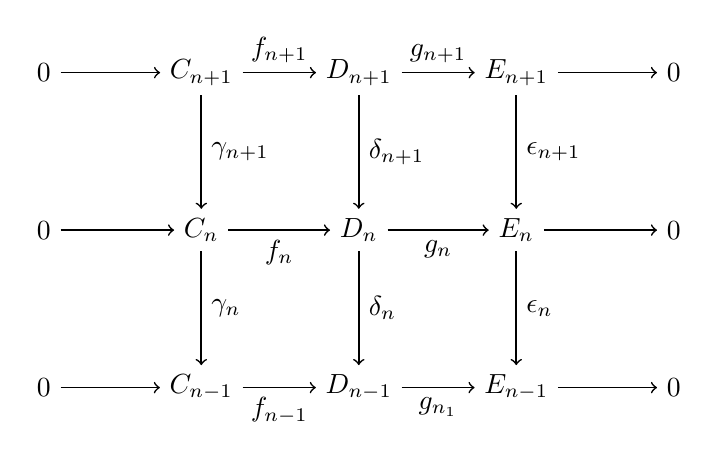
\begin{tikzpicture}[->,-latex, auto, main path/.style={->, semithick}, main node/.style={}]

\node	[main node]		(2) at (2,0)		{$0$};
\node	[main node]		(3) at (4,0)		{$C_{n+1}$};
\node [main node]		(4) at (6,0)		{$D_{n+1}$};
\node [main node]		(5) at (8,0)		{$E_{n+1}$};
\node	[main node]		(11) at (10,0)	{$0$};


\node	[main node]		(7) at (2,-2)		{$0$};
\node	[main node]		(8) at (4,-2)		{$C_n$};
\node [main node]		(9) at (6,-2)		{$D_n$};
\node [main node]		(10) at (8,-2)	{$E_n$};
\node [main node]		(13) at (10,-2)	{$0$};


\node	[main node]		(14) at (2,-4)	{$0$};
\node	[main node]		(15) at (4,-4)	{$C_{n-1}$};
\node [main node]		(16) at (6,-4)	{$D_{n-1}$};
\node [main node]		(17) at (8,-4)	{$E_{n-1}$};
\node [main node]		(18) at (10,-4)	{$0$};

\draw (2) edge [main path] node [auto] {$$} (3);
\draw (3) edge [main path] node [auto] {$f_{n+1}$} (4);
\draw (4) edge [main path] node [auto] {$g_{n+1}$} (5);
\draw (5) edge [main path] (11);

\draw (7) edge [main path] node [auto] {$$} (8);
\draw (8) edge [main path] node [auto, swap] {$f_n$} (9);
\draw (9) edge [main path] node [auto, swap] {$g_n$} (10);
\draw (10) edge [main path] (13);

\draw (14) edge [main path] node [auto] {$$} (15);
\draw (15) edge [main path] node [auto, swap] {$f_{n-1}$} (16);
\draw (16) edge [main path] node [auto, swap] {$g_{n_1}$} (17);
\draw (17) edge [main path] (18);

\draw (3) edge [main path] node [auto] {$\gamma_{n+1}$} (8);
\draw (4) edge [main path] node [auto] {$\delta_{n+1}$} (9);
\draw (5) edge [main path] node [auto] {$\epsilon_{n+1}$} (10);

\draw (8) edge [main path] node [auto] {$\gamma_{n}$} (15);
\draw (9) edge [main path] node [auto] {$\delta_{n}$} (16);
\draw (10) edge [main path] node [auto] {$\epsilon_{n}$} (17);
\end{tikzpicture}
\end{equation*}
\begin{itemize}
\item Define the connecting map $c_n:H_n(\mathbf{E})\to H_{n-1}(\mathbf{C})$ as follows:\\
Let $\overline{x}$ be a typical element of $H_n(\mathbf{E})$, with $x \in ker(\epsilon_n)=Z_n(\mathbf{E})$. Then as $g_n$ is surjective we can lift $x\in E_n$ to some element $y \in D_n$ such that $g_n(y)=x$. From the commutativity of the diagram, 
\begin{equation*}
g_{n-1}(\delta_n(y))=\epsilon_n(g_n(y))=\epsilon_n(x)=0,
\end{equation*}
since $x\in ker(\epsilon_n)$. Hence, $\delta_n(y)\in ker(g_{n-1})\cong im(f_{n-1})$. Then as $f_{n-1}$ is injective there exists some $z\in C_{n-1}$ such that $f_{n-1}(z)=\delta_n(y)$. Thus define $c_n(\overline{x})=\overline{z}$.(Note $z \in ker(\gamma_{n-1})$ as $\delta_{n-1}(\delta_n(y))=0$, then by commutivity $f_{n-2}(\gamma_{n-1}(z))=0$ and as $f_{n-2}$ is injective.)\\
\item Not dependent on choice of $x$ or $y$:
Say $y, y'\in D_n$ have images $g_n(y)=x$, $g_n(y')=x'$ where $x, x'\in ker(\epsilon_n)=Z_n(\mathbf{E})$ with $\overline{x}=\overline{x'}$. Thus $g_n(y)-g_n(y')\in im(\epsilon_{n+1})=B_n(\mathbf{E})$. Therefore, 
\begin{align*}
g_n(y-y')&=\epsilon_{n+1}(g_{n+1}(u))\text{, for some }u\in D_{n+1},\\
&=g_n(\delta_{n+1}(u)).
\end{align*}
Hence, $y-y'-\delta_{n+1}(u)=f_n(v)$ for some $v\in C_n$ by the injectivity of $f_n$. \\
If $f_{n-1}(z)=\delta_n(y)$ and $f_{n-1}(z')=\delta_n(y')$ then,
\begin{align*}
f_{n-1}(z-z')&=\delta_n(y-y'),\\
&=\delta_n(y-y'-\delta_(u))\text{, as $\delta_n(\delta_{n+1}(u))=0$ as chain complex,}\\
&=\delta_n(f_n(v)),\\
&=f_{n-1}(\gamma_n(v)),
\end{align*}
implying $z-z'=\gamma_n(v)\in im(\gamma_n)=B_{n-1}(\mathbf{C})$. Hence, $\overline{z}=\overline{z'}$ in $H_{n-1}(\mathbf{C})$.\\
\item Exactness at $H_n(\mathbf{C})$: $\quad H_{n+1}(\mathbf{E}) \xrightarrow{c_{n+1}} H_n(\mathbf{C})\xrightarrow{f_{\ast}}H_n(\mathbf{D})$\\
$im(c_{n+1})\subseteq ker(f_{\ast})$: We have $f_{\ast}(c_{n+1}(\overline{x}))=\overline{f_n(z)}$ for some $z\in C_n$. But,
\begin{equation*}
f_n(z)=\delta_{n+1}g^{-1}_{n+1}(x)\in B_{n+1}(\mathbf{D});
\end{equation*}
that is, $f_{\ast}(c_{n+1}(\overline{x})=0$.\\
$ker(f_{\ast})\subseteq im(c_{n+1})$: If $f_{\ast}(\overline{z})=\overline{f_n(z)}=\overline{0}$ then $f_n(z)=\delta_{n+1}(y')$ for some $y'\in D_{n+1}$. Since $g$ is a chain map,
\begin{align*}
\epsilon_{n+1}(g_{n+1}(y'))&=g_n(\delta_{n+1}(y')),\\
&=g_n(f_n(z)),\\
&=0, \text{ by exactness of the original sequence, }
\end{align*}
and so $g_{n+1}(y')\in Z_n(\mathbf{E})$. However,
\begin{align*}
c_{n+1}(\overline{g_{n+1}(y')})&=\overline{f^{-1}_n(\delta_{n+1}(g^{-1}_{n+1}(g_{n+1}(y'))))}, \\
&=\overline{f_n^{-1}\delta_{n+1}(y')}, \\
&=\overline{f_n^{-1}(f_n(z))}, \\
&=\overline{z}.
\end{align*}
\item Exactness at $H_n(\mathbf{D})$: $\quad H_n(\mathbf{C}) \xrightarrow{f_{\ast}} H_n(\mathbf{D}) \xrightarrow{g_{\ast}} H_n(\mathbf{E})$\\
$im(f_{\ast}) \subseteq ker(g_{\ast})$: True as,
\begin{equation*}
g_{\ast}f_{\ast}=(gf)_{\ast}=0_{\ast}=0.
\end{equation*}
$ker(g_{\ast})\subseteq im(f_{\ast})$: If $g_{\ast}(\overline{y})=\overline{g_n(y)}=\overline{0}$, then $g_n(y)=\epsilon_{n+1}$ for some $x'\in E_{n+1}$. However, $g$ is surjective meaning $x'=g_{n+1}$ for some $y'\in C_{n+1}$, hence, 
\begin{align*}
g_n(y)&=\epsilon_{n+1}(g_{n+1}(y')),\\
&=g_n(\delta_{n+1}(y')),
\end{align*} 
since $g$ is a chain map and so $ g_n(y-\delta){n+1}(y')=0$. By exactness, there is $z\in C_n$ with $f_n(z)=y-\delta_{n+1}(y')$. Now $z\in Z_n(\mathbf{C})$ because,
\begin{align*}
f_{n-1}(\gamma_n(z))&=\delta_n(f_n(z)), \\
&=\delta_n(y-\delta_{n+1}(y')), \\
&=\delta_n(y)-\delta_n(\delta_{n+1}(y')), \\
&=0, \text{ as } y\in Z_n(\mathbf{C})\text{ and } \delta_n\delta_{n+1}=0,
\end{align*}
then because $f_{n-1}$ is injective, $\gamma_n(z)=0$. Therefore, 
\begin{align*}
f_{\ast}(\overline{z})&=\overline{f_n(z)}, \\
&=\overline{y-\delta_{n+1}(y')}, \\
&=\overline{y}.
\end{align*}
\item Exactness at $H_n(\mathbf{E})$: $\quad H_n(\mathbf{D}) \xrightarrow{g_{\ast}} H_n(\mathbf{E}) \xrightarrow{c_n} H_{n-1}(\mathbf{C})$\\
$im(g_{\ast})\subseteq ker(c_n)$: If $g_{\ast}(\overline{y})=\overline{g_n(y)} \in im(g_{\ast})$, then $c_n(\overline{g_n(y')})=\overline{z}$ where, 
\begin{equation*}
f_{n-1}(z)=\delta_n(g_n^{-1}(g_n(y'))).
\end{equation*}
Since this formula is independent of the choice of lifting of $g_n(y')$, let us choose $g_n^{-1}(g_n(y'))=y'$. Now $\delta_n(g^{-1}_n(g_n(y'))=\delta_n(y')=0$ because $y'\in Z_n(\mathbf{D})$. Thus, $f_{n-1}(z)=0$ and hence $z=0$ because $f_{n-1}$ is injective. \\
$ker(c_n)\subseteq im(g_{\ast})$: If $c_n(x)=\overline{0}$, then $z'=f_{n-1}^{-1}=f_{n-1}^{-1}(\delta_n(g_n^{-1}(x)))\in B_n(\mathbf{C})$, that is $z'=\gamma_n(z)$ for some $z\in C_n$. However, 
\begin{align*}
f_{n-1}(z')&=f_{n-1}(\gamma_n(z)), \\
&=\delta_n(f_n(z)), \\
&=\delta_n(g^{-1}_n(x)), 
\end{align*}
so that $\delta_n(g_n^{-1}-f_n(z))=0$, that is $g_n^{-1}-f_n(z) \in ker(\delta_n)$. Exactness of the original sequence gives $g_nf_n=0$, so that,
\begin{align*}
g_{\ast}(\overline{g_n^{-1}(x)-f_n(z)})&=\overline{g_n(g_n^{-1}(x)-gn(f_n(z)}, \\
&=\overline{x}.
\end{align*}
\end{itemize}
\end{proof}
% Maybe include an example, going to take some time to work one out...

Note that this report is following Crawley-Boevey's example in \cite{CB1} by proving the Long Exact Sequence theorem directly and taking the Snake Lemma as a corollary, unlike in other reading material, like \cite{Weibel} where the Long Exact Sequence is given as a corollary of the Snake Lemma. If the reader would like a direct proof of the Snake Lemma, we direct them, as Weibel does in \cite{Weibel}, to \emph{It's My Turn} (Rastar-Martin Elfand Studios, 1980), where a proof is given in the beginning of the movie.
% This might need a rewrite

\begin{cor} (Snake Lemma)\\
If you have a commutative diagram with exact rows, 
\begin{equation*}
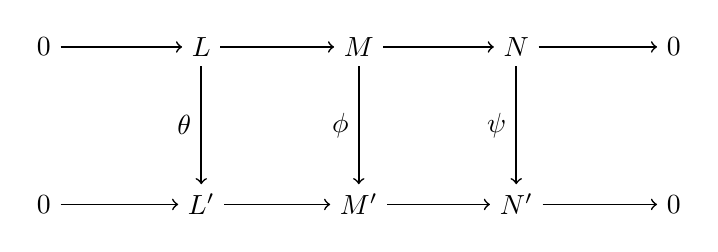
\begin{tikzpicture}[->,-latex, auto, main path/.style={->, semithick}, main node/.style={}]

\node	[main node]		(2) at (2,0)		{$0$};
\node	[main node]		(3) at (4,0)		{$L$};
\node [main node]		(4) at (6,0)		{$M$};
\node [main node]		(5) at (8,0)		{$N$};
\node	[main node]		(11) at (10,0)	{$0$};


\node	[main node]		(7) at (2,-2)		{$0$};
\node	[main node]		(8) at (4,-2)		{$L'$};
\node [main node]		(9) at (6,-2)		{$M'$};
\node [main node]		(10) at (8,-2)	{$N'$};
\node [main node]		(13) at (10,-2)	{$0$};

\draw (2) edge [main path] node [auto] {$$} (3);
\draw (3) edge [main path]node [auto] {$$} (4);
\draw (4) edge [main path] node [auto] {$$} (5);
\draw (5) edge [main path] (11);

\draw (7) edge [main path] node [auto] {$$} (8);
\draw (8) edge [main path] (9);
\draw (9) edge [main path] (10);
\draw (10) edge [main path] (13);


\draw (3) edge [main path] node [auto, swap] {$\theta$} (8);
\draw (4) edge [main path] node [auto, swap] {$\phi$} (9);
\draw (5) edge [main path] node [auto, swap] {$\psi$} (10);

\end{tikzpicture}
\end{equation*}
you get an exact sequence, 
\begin{equation*}
0\xrightarrow{}ker(\theta)\xrightarrow{}ker(\phi)\xrightarrow{}ker(\psi)\xrightarrow{}coker(\theta)\xrightarrow{}coker(\phi)\xrightarrow{}coker(\psi)\xrightarrow{}0
\end{equation*}
\end{cor}
\begin{proof}
Consider $L\to L'$, $M\to M'$ and $N\to N'$ as chain complexes and use Theorem \ref{longexactseqthm}.
\end{proof}

\begin{rem} \label{longexactseqcochainrem}
A short exact sequence of cochain complexes $0\xrightarrow{}\mathbf{C}\xrightarrow{}\mathbf{D} \xrightarrow{} \mathbf{E}\xrightarrow{}0$ gives a long exact sequence,
\begin{equation*}
\dots \xrightarrow{} H^{n-1}(\mathbf{E})\xrightarrow{}H^n(\mathbf{C})\xrightarrow{}H^n(\mathbf{D})\xrightarrow{}H^n(\mathbf{E})\xrightarrow{} H^{n+1}(\mathbf{C})\xrightarrow{} H^{n+1}(\mathbf{D})\xrightarrow{} \dots
\end{equation*}
by renumbering in Theorem \ref{longexactseqthm}.
\end{rem}

%%%%%%%%%%%%%%%%%%%%%%%%%%%%%%%%%%%%%%%%%%%%%%%%%%%%%%%
%%%%%%%%%%%%%%		 Homotopy and Quasi-Isomorphism 		%%%%%%%%%%%%%%%%%
%%%%%%%%%%%%%%%%%%%%%%%%%%%%%%%%%%%%%%%%%%%%%%%%%%%%%%%

\section{Homotopy and Quasi-Isomorphism}

For this section the report relies heavily on \cite{CB1}, with some added details, such as the definition for null homotopic and the diagram, come from \cite{Weibel} and \cite{Rotman}. However, all examples are original work.

\begin{mydef}
If $f,g:\mathbf{C} \to \mathbf{D}$  are chain maps, then $f$ and $g$ are \emph{homotopic}, denoted $f\simeq g$, if for each $n$ there are maps $h_n: C_n \to D_{n+1}$ such that,
\begin{equation*}
f_n-g_n=h_{n-1}\gamma_n + \delta_{n+1}h_n,
\end{equation*}
where the maps are defined
,
\begin{equation*}
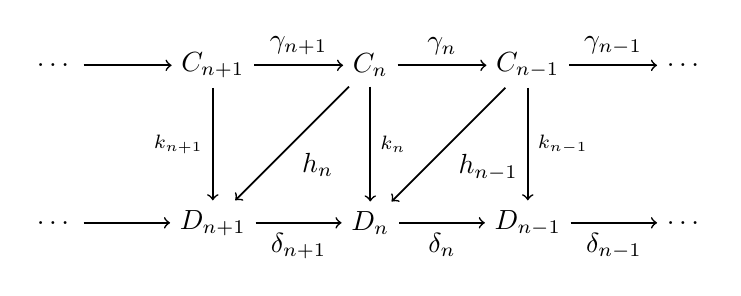
\begin{tikzpicture}[->,-latex, auto, main path/.style={->, semithick}, main node/.style={}]
\node	[main node]		(2) at (2,0)		{\dots};
\node	[main node]		(3) at (4,0)		{$C_{n+1}$};
\node [main node]		(4) at (6,0)		{$C_n$};
\node [main node]		(5) at (8,0)		{$C_{n-1}$};
\node	[main node]		(11) at (10,0)	{\dots};

\node	[main node]		(7) at (2,-2)		{\dots};
\node	[main node]		(8) at (4,-2)		{$D_{n+1}$};
\node [main node]		(9) at (6,-2)		{$D_n$};
\node [main node]		(10) at (8,-2)	{$D_{n-1}$};
\node [main node]		(13) at (10,-2)	{\dots};

\draw (2) edge [main path] node [auto] {$$} (3);
\draw (3) edge [main path] node [auto] {$\gamma_{n+1}$} (4);
\draw (4) edge [main path] node [auto] {$\gamma_n$} (5);
\draw (5) edge [main path] node [auto] {$\gamma_{n-1}$} (11);

\draw (7) edge [main path] node [auto] {$$} (8);
\path (8) edge [main path] node [auto, swap] {$\delta_{n+1}$} (9);
\draw (9) edge [main path] node [auto, swap] {$\delta_n$} (10);
\draw (10) edge [main path] node [auto, swap] {$\delta_{n-1}$} (13);

\draw (3) edge [main path] node [auto, swap] {$\scriptstyle{k_{n+1}}$} (8);
\draw (4) edge [main path] node [auto] {$\scriptstyle{k_n}$} (9);
\draw (5) edge [main path] node [auto] {$\scriptstyle{k_{n-1}}$} (10);

\draw (4) edge [main path] node [auto] {$h_n$} (8);
\draw (5) edge [main path] node [auto] {$h_{n-1}$} (9);
\end{tikzpicture}
\end{equation*}
with $k_n$ representing either $f_n$ or $g_n$.\\
A chain map $f:\mathbf{C} \to \mathbf{D}$ is considered \emph{null-homotopic} if $f \simeq 0$, where $0$ is the zero chain map.
\end{mydef}

\begin{eg}
Consider the two chain complexes,
\begin{equation*}
\mathbf{C}: \quad \dots \xrightarrow{} 0 \xrightarrow{} \bb{Z} \xrightarrow{3} \bb{Z} \xrightarrow{} 0 \xrightarrow{} \dots \quad \& \quad \mathbf{D}: \quad \dots \xrightarrow{} \frac{\bb{Z}}{9\bb{Z}} \xrightarrow{3} \frac{\bb{Z}}{9\bb{Z}} \xrightarrow{3} \frac{\bb{Z}}{9\bb{Z}} \xrightarrow{} \dots,
\end{equation*}
such that $C_1,C_0=\bb{Z}$ and $D_n=\sfrac{\bb{Z}}{9\bb{Z}}$. Then the two chain maps $f, g:\mathbf{C} \to \mathbf{D}$, where $f_0, f_1: x \mapsto 4x+9\bb{Z}$ and $g_0, g_1: x \to x+9\bb{Z}$ are homotopic where $h_0: \bb{Z} \to \sfrac{\bb{Z}}{9\bb{Z}}, x \to x+9\bb{Z}$ and $h_1: \bb{Z} \to \sfrac{\bb{Z}}{9\bb{Z}}, x \mapsto 3x +9\bb{Z}$.
\end{eg}

%Reference
\begin{prop} \label{homotopyhomologyprop}
If $f,g:\mathbf{C}\to \mathbf{D}$ are homotopic then for each $n$ they induce exactly the same map $H_n(\mathbf{C})\to H_n(\mathbf{D})$.
\end{prop}
\begin{proof}
Let $\overline{x} \in H_n(\mathbf{C})$ such that $x\in Z_n(\mathbf{C})$. Then,
\begin{align*}
H_n(f)(\overline{x})-H_n(g)(\overline{x})&= \overline{f_n(x)} - \overline{g_n(x)},\\
&= \overline{h_{n-1}\gamma_n(x)-\delta_{n+1}h_n(x)},\\
&=\overline{\delta_{n+1}h_n(x)}, \text{ as }x\in Z_n(\mathbf{C})=ker(\gamma_n),\\
&=0, \text{ as } \delta_{n+1}h_n(x)\in B_n(\mathbf{D})=im(\delta_{n+1}).
\end{align*}
\end{proof}

\begin{prop} %Not sure whether to keep this propn in. May get rid.
If $f,g: \mathbf{C}\to \mathbf{D}$ are homotopic and $N$ is an $R$-module, then the induced cochain maps $Hom(\mathbf{D}, N) \to Hom(\mathbf{C},N)$ are homotopic.
\end{prop}
\begin{proof}
A homotopy is given by maps $h_n:C_n\to D_{n+1}$ such that, 
\begin{equation*}
f_n-g_n=h_{n-1}\gamma_n + \delta_{n+1}h_n.
\end{equation*}
Let $h^n:Hom(\mathbf{D},N)^n \to Hom(\mathbf{C}, N)^{n-1}$ be $Hom(h_{n-1}, N)$, as $Hom(D, N)^n \cong Hom(D_n, N)$ and $Hom(C, N)^{n-1} \cong Hom(C_{n-1}, N)$.
\end{proof}

\begin{mydef}
A chain map $f:\mathbf{C} \to \mathbf{D}$ is a \emph{homotopy equivalence} if there is a chain map $g:\mathbf{D} \to \mathbf{C}$ such that $gf$ and $fg$ are homotopic to the respective identity maps of $\mathbf{C}$ and $\mathbf{D}$.\\
If there exists a homotopy equivalence, $f:\mathbf{C} \to \mathbf{D}$, $\mathbf{C}$ and $\mathbf{D}$ are said to be \emph{homotopy equivalent}.
\end{mydef}

% Would like an example here.

\begin{rem}
The reader is advised not to confuse these definitions: Note that the two chain maps $f,g:\mathbf{C} \to \mathbf{D}$ can be homotopic, whilst two chain complexes $\mathbf{C}, \mathbf{D}$ can be homotopy equivalent.
\end{rem}

\begin{prop}
A homotopy equivalence $f:\mathbf{C} \to \mathbf{D}$ of chain complexes induces a homotopy equivalence of cochain complexes $Hom(\mathbf{D},N) \to Hom(\mathbf{C},N)$. In particular, $H^n(\mathbf{D}, N) \cong H^n(\mathbf{C}, N)$.
\end{prop}
\begin{proof}
Omitted.
%Given as clear in \cite{CB1}, may prove later.
\end{proof}

\begin{mydef}
A chain map $f:\mathbf{C} \to \mathbf{D}$ is a \emph{quasi-isomorphism} if for each $n$ the map $H_n(\mathbf{C}) \to H_n(\mathbf{D})$ is an isomorphism.
\end{mydef}

\begin{prop} \label{homequivisomprop}
If $f:\mathbf{C} \to \mathbf{D}$ is a homotopy equivalence then it is a quasi-isomorphism.
\end{prop}
\begin{proof}
Assume that $f: \mathbf{C} \to \mathbf{D}$ is a homotopy equivalence, then there exists some chain map $g: \mathbf{D} \to \mathbf{C}$ such that $fg \simeq id_{\mathbf{D}}$ and $gf\simeq id_{\mathbf{C}}$. By Proposition \ref{homotopyhomologyprop}, since $fg \simeq id_{\mathbf{D}}$ then they both induce the same map $H_n(\mathbf{D}) \to H_n(\mathbf{D})$ and similarly $gf$ and $id_{\mathbf{C}}$ induce the same map $H_n(\mathbf{C}) \to H_n(\mathbf{C})$. Hence, $f$ induces an isomorphism $H_n(\mathbf{C}) \to H_n(\mathbf{D})$ as it has an inverse and so is a quasi-isomorphism.
\end{proof}

\begin{eg}
This example shows that the converse to Proposition \ref{homequivisomprop} is not true. Consider the chain complexes, 
\begin{equation*}
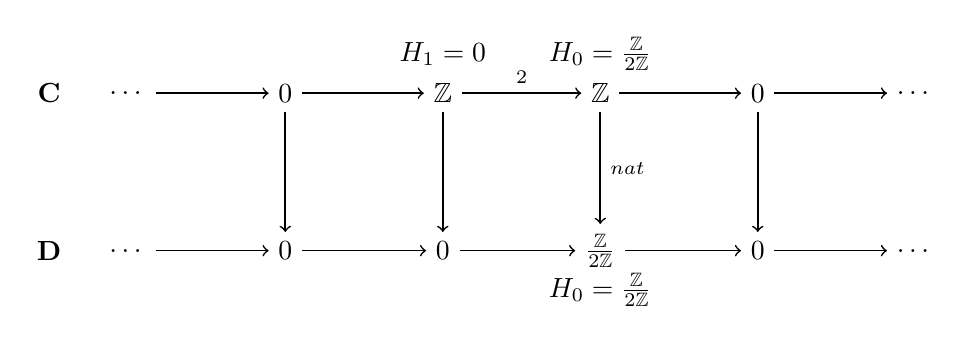
\begin{tikzpicture}[->,-latex, auto, main path/.style={->, semithick}, main node/.style={}]
\node [main node]		(1) at (1,0)		{$\mathbf{C}$};
\node	[main node]		(2) at (2,0)		{\dots};
\node	[main node]		(3) at (4,0)		{$0$};
\node [main node]		(4) at (6,0)		{$\bb{Z}$};
\node [main node]		(5) at (8,0)		{$\bb{Z}$};
\node	[main node]		(11) at (10,0)	{$0$};
\node [main node]		(12) at (12,0)	{\dots};

\node [main node]		(6) at (1,-2)		{$\mathbf{D}$};
\node	[main node]		(7) at (2,-2)		{\dots};
\node	[main node]		(8) at (4,-2)		{$0$};
\node [main node]		(9) at (6,-2)		{$0$};
\node [main node]		(10) at (8,-2)	{$\frac{\bb{Z}}{2\bb{Z}}$};
\node [main node]		(13) at (10,-2)	{$0$};
\node [main node] 		(14) at (12, -2)	{\dots};

\node [main node] 		(15) at (8,0.5)	{$H_0=\frac{\bb{Z}}{2\bb{Z}}$};
\node [main node]		(16) at (6,0.5)	{$H_1=0$};
\node [main node]		(17) at (8,-2.5)	{$H_0=\frac{\bb{Z}}{2\bb{Z}}$};

\draw (2) edge [main path] node [auto] {$$} (3);
\draw (3) edge [main path] node [auto] {$$} (4);
\draw (4) edge [main path] node [auto] {$\scriptstyle{2}$} (5);
\draw (5) edge [main path] node [auto] {$$} (11);
\draw (11) edge [main path] (12);

\draw (7) edge [main path] node [auto] {$$} (8);
\path (8) edge [main path] node [auto, swap] {$$} (9);
\draw (9) edge [main path] node [auto, swap] {$$} (10);
\draw (10) edge [main path] node [auto, swap] {$$} (13);
\draw (13) edge [main path] (14);

\draw (3) edge [main path] node [auto, swap] {$$} (8);
\draw (4) edge [main path] node [auto] {$$} (9);
\draw (5) edge [main path] node [auto] {$\scriptstyle{nat}$} (10);
\draw (11) edge [main path] (13);
\end{tikzpicture}
\end{equation*}
and so $H_0(\mathbf{C})=\frac{\bb{Z}}{2\bb{Z}}=H_0(\mathbf{D})$ and so $f$ is a quasi-isomorphism. However, it is not a homotopy equivalence.
\end{eg}

\begin{mydef}
A chain complex $\mathbf{C}$ is \emph{contractible} if it is homotopy equivalent to the zero complex. \\
Equivalent condition: $id_{\mathbf{C}}$ is homotopic to $0_{\mathbf{C}}$.\\
Equivalent condition: There are maps $h_n: C_n \to C_{n+1}$ with,
\begin{equation*}
id_{C_n} = h_{n-1}\gamma_n + \delta_{n+1}h_n,\text{ for all } n.
\end{equation*}
This is called a \emph{contracting homotopy}.
\end{mydef}

\begin{thm}
A chain complex $\mathbf{C}$ is contractible if and only if it is acyclic and all of the short exact sequences,
\begin{equation*}
0 \xrightarrow{} Z_(\mathbf{C} \xrightarrow{\iota_n} C_n \xrightarrow{\gamma_n} B_{n-1}(\mathbf{C})\xrightarrow{} 0,
\end{equation*}
are split, where $\iota_n$ is the inclusion.
\end{thm}
\begin{proof}
$\Rightarrow$: If $\mathbf{C}$ is contractible then it is quasi-isomorphic to the zero complex, so acyclic by Proposition \ref{homequivisomprop}. Let $h$ be the contracting homotopy. Let $s:B_{n-1}(\mathbf{C})\to C_n$ be the restriction of $h_{n-2}:C_{n-1} \to C_n$. If $x\in B_{n-1}(\mathbf{C})=im(\gamma_n)$,
\begin{align*}
B_{n-1}(\mathbf{C}\ni x&=id_{C_{n-1}}(x),\\
&=(h_{n-1}\gamma_{n-1} + \gamma_nh_{n-1})(x),\\
&=h_{n-2}(\gamma_{n-1}(x))+\gamma_n(h_{n-1}(x)),\\
&=\gamma_n(h_{n-1}(x)),\\
&=\gamma_n(s(x)).
\end{align*}
Thus $s$ makes $\gamma_n$ is a retraction in the short exact sequence.
$\Leftarrow$: Now suppose that $\mathbf{C}$ is acyclic and all the exact sequences are split. Then for all $n$ there are sections,
\begin{equation*}
s_{n-1}: B_{n-1}(\mathbf{C}) \to C_n.
\end{equation*}
If $x\in C_n$ then $x-s_{n-1}\gamma_nx\in Z_n(\mathbf{C})=B_n(\mathbf{C})$ so we can define a function $h_n: C_n \to C_{n-1}$ by,
\begin{equation*}
h_n(x)=s_n(x-s_{n-1}\gamma_nx).
\end{equation*}
Then,
\begin{align*}
(h_{n-1}\gamma_n + \gamma_{n+1}h_n)(x)&=s_{n-1}(\gamma_nx-s_{n-2}\gamma_{n-1}\gamma_nx) + \gamma_{n+1}s_n(x - s_{n-1}\gamma_nx),\\
&=s_{n-1}\gamma_nx +(x-s_{n-1}\gamma_nx), \text{ as } s_n \text{ is a section},\\
&=x.
\end{align*}
\end{proof}





%%%%%%%%%%%%%%%%%%%%%%%%%%%%%%%%%%%%%%%%%%%%%%%%%%%%%%%
%%%%%%%%%%%%%%		 Projective and Injective Resolutions 		%%%%%%%%%%%%%%%%%%
%%%%%%%%%%%%%%%%%%%%%%%%%%%%%%%%%%%%%%%%%%%%%%%%%%%%%%%

\section{Projective and Injective Resolutions}

In this section we look at projective and injective modules and resolutions, for this the reader will need some prior knowledge of free modules, which will not be covered in this report. The reader is advised to look at \cite{Stamm}, \cite{Weibel} and \cite{Rotman} for more information regarding free modules.\\
The following properties for projective modules come from \cite{CB1} with added details from either my own work or \cite{Rotman}. In order to have a clear definition of a projective modules, rather than as a culmination of properties, we have promoted the first property from \cite{CB1} to a definition and to aid this we give a separate defintion for a lifting as in \cite{Rotman}.

\begin{mydef}
Suppose we have a map $g:M \to N$ then a \emph{lifting} of a map $p:A \to N$ is a map $q:A\to M$ with $gq=p$, i.e. the following diagram commutes.
\begin{equation*}
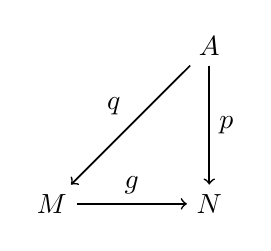
\begin{tikzpicture}[->,-latex, auto, main path/.style={->, semithick}, main node/.style={}]
\node	[main node]		(1) at (0,0)		{$M$};
\node	[main node]		(2) at (2,0)		{$N$};
\node [main node]		(3) at (2,2)		{$A$};

\draw (1) edge [main path] node [auto] {$g$} (2);
\draw (3) edge [main path] node [auto] {$p$} (2);
\draw (3) edge [main path] node [auto, swap] {$q$} (1);
\end{tikzpicture}
\end{equation*}
\end{mydef}

\begin{mydef}
A module $P$ is \emph{projective} if, whenever $g:M\to N$ is surjective and $p:P\to N$ is any map, there exists a lifting $q:P \to M$ making the following diagram commutes:
\begin{equation*}
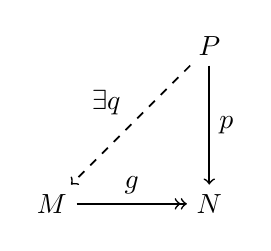
\begin{tikzpicture}[->,-latex, auto, main path/.style={->, semithick}, main node/.style={}]
\node	[main node]		(1) at (0,0)		{$M$};
\node	[main node]		(2) at (2,0)		{$N$};
\node [main node]		(3) at (2,2)		{$P$};

\draw (1) edge [->>, semithick] node [auto] {$g$} (2);
\draw (3) edge [main path] node [auto] {$p$} (2);
\draw (3) edge [dashed, ->, semithick] node [auto, swap] {$\exists q$} (1);
\end{tikzpicture}
\end{equation*}
\end{mydef}

\begin{prop} \label{projectiveprop}
The following for a module $P$ are equivalent:
\begin{description}
\item [(i)] P is projective.
\item [(ii)] The sequence $0\xrightarrow{}Hom(P, L)\xrightarrow{}Hom(P, M)\xrightarrow{}Hom(P, N)\xrightarrow{}0$ is exact for any short exact sequence $0\xrightarrow{}L\xrightarrow{}M\xrightarrow{}N\xrightarrow{}0$.
\item [(iii)]Any short exact sequence $0\xrightarrow{}L\xrightarrow{}M\xrightarrow{}P\xrightarrow{}0$ splits.
\item [(iv)]$P$ is isomorphic to a direct summand of free modules.
\end{description}
\end{prop}
\begin{proof} (i) $\Rightarrow$ (ii): As $P$ is projective we have that,
\begin{equation*}
\begin{tikzpicture}[->,-latex, auto, main path/.style={->, semithick}, main node/.style={}]
\node	[main node]		(1) at (0,0)		{$M$};
\node	[main node]		(2) at (2,0)		{$N$};
\node [main node]		(3) at (2,2)		{$P$};
\node [main node]		(4) at (-2, 0)		{$L$};
\node [main node]		(5) at (-4, 0)		{$0$};
\node [main node]		(6) at (4, 0)		{$0$};

\draw (1) edge [->>, semithick] node [auto] {$g$} (2);
\draw (3) edge [main path] node [auto] {$p$} (2);
\draw (3) edge [dashed, ->, semithick] node [auto, swap] {$\exists q$} (1);
\draw (4) edge [main path] node [auto] {$f$} (1);
\draw (5) edge [main path] (4);
\draw (2) edge [main path] (6);
\end{tikzpicture}
\end{equation*}
Hence, we have $q\in Hom(P,M)$ such that $gq=p\in Hom(P,N)$ which can also we written $p=gq=g_{\ast}(q)\in im(g_{\ast})$, defining a surjective map, $g_{\ast}: Hom(P,M) \to Hom(P,N)$. Thus,
\begin{equation*}
0\xrightarrow{}Hom(P,L) \xrightarrow{}Hom(P,M)\xrightarrow{g_{\ast}}Hom(P,N)\xrightarrow{}0
\end{equation*}
is exact by Proposition \ref{exactpropertiesprop}.\\
(ii) $\Rightarrow$ (iii): By assumption, if we have the short exact sequence $0\xrightarrow{}L\xrightarrow{}M\xrightarrow{}P\xrightarrow{}0$ then we have an exact sequence,
\begin{equation*}
0\xrightarrow{}Hom(P,L) \xrightarrow{}Hom(P,M)\xrightarrow{}Hom(P,P)\xrightarrow{}0.
\end{equation*}
Then we can lift the identity map $id_P\in Hom(P,P)$ to some $q\in Hom(P,M)$, such that:
\begin{equation*}
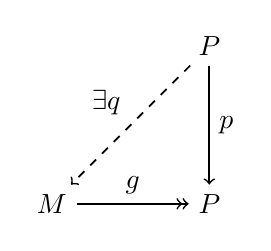
\begin{tikzpicture}[->,-latex, auto, main path/.style={->, semithick}, main node/.style={}]
\node	[main node]		(1) at (0,0)		{$M$};
\node	[main node]		(2) at (2,0)		{$P$};
\node [main node]		(3) at (2,2)		{$P$};

\draw (1) edge [->>, semithick] node [auto] {$g$} (2);
\draw (3) edge [main path] node [auto] {$p$} (2);
\draw (3) edge [dashed, ->, semithick] node [auto, swap] {$\exists q$} (1);
\end{tikzpicture}
\end{equation*}
Thus $g:M\to P$ is a retraction as we have $q:P\to M$ such that $gq=id_P$. Hence, $0\xrightarrow{}L\xrightarrow{}M\xrightarrow{}P\xrightarrow{}0$ splits by Lemma \ref{splittinglem}.\\
(iii)$\Rightarrow$ (iv): By choosing a generating set of $P$ we get a surjection from a free module $F$ onto $P$, $g:F\to P$, and this gives the short exact sequence, 
\begin{equation*}
0\xrightarrow{}ker(g)\xrightarrow{}F\xrightarrow{g}P\xrightarrow{}0,
\end{equation*}
and this splits by assumption. Hence, $F\cong ker(g)\oplus P$ and so $P$ is a direct summand of $F$ by Corollary \ref{MLNcor}.\\
(iv) $\Rightarrow$ (i): By assumption, $P$ is a direct summand of $F$ and so there are maps $r: F \to P$ and $s: P \to F$ with $rs=id_P$. Now consider the diagram, 
\begin{equation*}
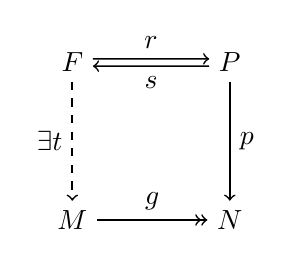
\begin{tikzpicture}[->,-latex, auto, main path/.style={->, semithick}, main node/.style={}]
\node	[main node]		(1) at (0,0)		{$M$};
\node	[main node]		(2) at (2,0)		{$N$};
\node [main node]		(3) at (2,2)		{$P$};
\node [main node]		(4) at (0,2)		{$F$};

\draw (1) edge [->>, semithick] node [auto] {$g$} (2);
\draw (3) edge [main path] node [auto] {$p$} (2);
\draw (4) edge [dashed, ->, semithick] node [auto, swap] {$\exists t$} (1);
\path (4.10) edge [main path] node [auto] {$r$} (3.170);
\path (3.190) edge [main path] node [auto] {$s$} (4.-10);
\end{tikzpicture}
\end{equation*}
where $g$ is surjective. The composite map $pr: F \to N$; since $F$ is free, it is surjective, and so there is a map $t: F \to M$ with $gt=pr$. Define $q: P \to M$ by $q=ts$ and then we can see that $gq=p$ as,
\begin{equation*}
gq=gts=prs=pid_P=p.
\end{equation*}
Hence $P$ is projective.
\end{proof}

Now we have established some properties of projective modules we can prove a corollary of the Long Exact Sequence Theorem in \cite{CB1}.

\begin{cor} (Corollary to Theorem \ref{longexactseqthm})\\
If $\mathbf{P}$ is a chain complex of projective $R$-modules and $0\xrightarrow{}L\xrightarrow{}M\xrightarrow{}N\xrightarrow{}0$ is a short exact sequence of $R$-modules then you get a long exact sequence in cohomology.
\begin{equation*}
\dots \xrightarrow{} H^{n-1}(\mathbf{P}, N) \xrightarrow{} H^n(\mathbf{P}, L) \xrightarrow{} H^n(\mathbf{P}, M) \xrightarrow{} H^n(\mathbf{P}, N) \xrightarrow{} H^{n+1}(\mathbf{P}, L) \xrightarrow{} \dots
\end{equation*}
\end{cor}
\begin{proof}
Since $P_n$ is projective for every $n$, Proposition \ref{projectiveprop}, tells us we get an exact sequence,
\begin{equation*}
0\xrightarrow{} Hom(P_n, L) \xrightarrow{} Hom(P_n, M) \xrightarrow{} Hom(P_n, N) \xrightarrow{} 0.
\end{equation*}
Then use Remark \ref{longexactseqcochainrem}.
\end{proof}

As with projective modules we will use the first property given in \cite{CB1} to define injective modules, and then provide the properties as in \cite{CB1} with some details from \cite{Rotman}.

\begin{mydef}
A module $I$ is \emph{injective} if, whenever $f: L \to M$ is an injection, there exists a map $j: M \to I$ which extends any map $i: M \to I$, making the following diagram commute.
\begin{equation*}
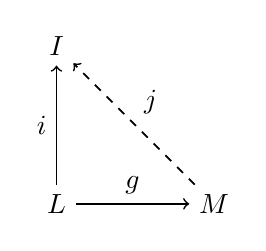
\begin{tikzpicture}[->,-latex, auto, main path/.style={->, semithick}, main node/.style={}]
\node	[main node]		(1) at (0,0)		{$L$};
\node	[main node]		(2) at (2,0)		{$M$};
\node [main node]		(3) at (0,2)		{$I$};

\draw (1) edge [main path] node [auto] {$g$} (2);
\draw (1) edge [main path] node [auto] {$i$} (3);
\draw (2) edge [dashed, ->, semithick] node [auto, swap] {$j$} (3);
\end{tikzpicture}
\end{equation*}
\end{mydef}

\begin{prop}
The following properties of a module $I$ are equivalent:
\begin{description}
\item [(i)] $I$ is injective.
\item [(ii)] The sequence $0\xrightarrow{} Hom(N, I) \xrightarrow{} Hom(M, I) \xrightarrow{} Hom(L, I) \xrightarrow{} 0$ is exact for any short exact sequence $0\xrightarrow{} L \xrightarrow{} M\xrightarrow{} N \xrightarrow {} 0$.
\item [(iii)] Any short exact sequence $0 \xrightarrow{} I \xrightarrow{} M \xrightarrow{} N \xrightarrow{}0$ splits.
\end{description}
\end{prop}
\begin{proof}
(i) $\Rightarrow$ (ii) $\Rightarrow$ (iii): Dual to Proposition \ref{projectiveprop}  for projectives.
(iii) $\Rightarrow$ (i): Consider the $0\xrightarrow{}L\xrightarrow{}M\xrightarrow{}\sfrac{M}{L} \xrightarrow{} 0$ and construct it's pushout along $\theta: L \to I$:
\begin{equation*}
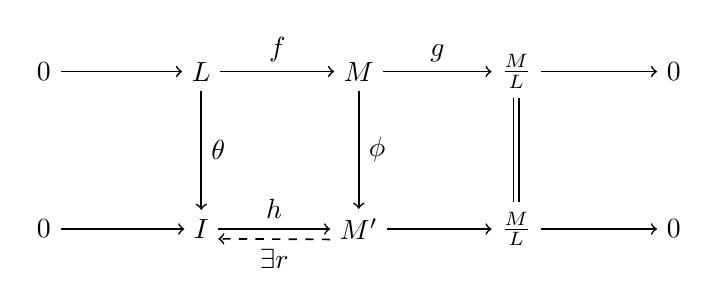
\begin{tikzpicture}[->,-latex, auto, main path/.style={->, semithick}, main node/.style={}]

\node	[main node]		(2) at (2,0)		{$0$};
\node	[main node]		(3) at (4,0)		{$L$};
\node [main node]		(4) at (6,0)		{$M$};
\node [main node]		(5) at (8,0)		{$\frac{M}{L}$};
\node	[main node]		(11) at (10,0)	{$0$};

\node	[main node]		(7) at (2,-2)		{$0$};
\node	[main node]		(8) at (4,-2)		{$I$};
\node [main node]		(9) at (6,-2)		{$M'$};
\node [main node]		(10) at (8,-2)	{$\frac{M}{L}$};
\node [main node]		(13) at (10,-2)	{$0$};

\draw (2) edge [main path] node [auto] {$$} (3);
\draw (3) edge [main path] node [auto] {$f$} (4);
\draw (4) edge [main path] node [auto] {$g$} (5);
\draw (5) edge [main path] (11);

\draw (7) edge [main path] node [auto] {$$} (8);
\path (8.0) edge [main path] node [auto] {$h$} (9.180);
\path (9.200) edge [dashed, ->, semithick] node [auto] {$\exists r$} (8.330);
\draw (9) edge [main path] node [auto, swap] {$$} (10);
\draw (10) edge [main path] (13);

\draw (3) edge [main path] node [auto] {$\theta$} (8);
\draw (4) edge [main path] node [auto] {$\phi$} (9);
\draw (5) edge [-, semithick, double, double distance=1.5pt](10);
\end{tikzpicture}
\end{equation*}
By assumption $0\xrightarrow{}I\xrightarrow{}M'\xrightarrow{}\sfrac{M}{L}\xrightarrow{}0$ splits and so $h:I \to M'$ has a retraction $r:M'\to I$. Then,
\begin{equation*}
r\phi f=rh\theta=\theta,
\end{equation*}
so $r\phi : M \to I$ extends $\theta: L \to I$. Hence $I$ is injective.
\end{proof}

\begin{mydef}
If $M$ is an $R$-module, then a \emph{projective resolution} of $M$ is an exact sequence, 
\begin{equation*}
\mathbf{P}: \quad \dots \xrightarrow{} P_2 \xrightarrow{d_2} P_1 \xrightarrow{d_1} P_0 \xrightarrow{\epsilon} M \xrightarrow{} 0
\end{equation*}
where each $P_i$ is a projective module.
\end{mydef}

\begin{prop}
A projective resolution $\mathbf{P}$ of $M$ is equivalent to giving a non-negative chain complex $\mathbf{P}_{\bullet}$ of projective modules and a quasi-isomorphism $f: \mathbf{P}_{\bullet} \to \mathbf{M}$, where all the $f_n$ are trivial apart from $f_0: P_0 \twoheadrightarrow M$.
\end{prop}
\begin{proof}
Consider the diagram,
\begin{equation*}
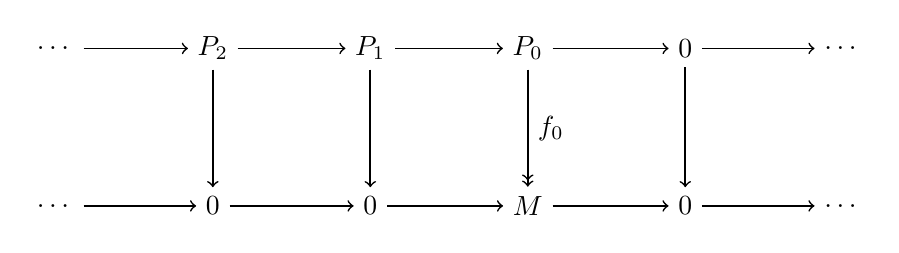
\begin{tikzpicture}[->,-latex, auto, main path/.style={->, semithick}, main node/.style={}]
\node	[main node]		(2) at (2,0)		{$\dots$};
\node	[main node]		(3) at (4,0)		{$P_2$};
\node [main node]		(4) at (6,0)		{$P_1$};
\node [main node]		(5) at (8,0)		{$P_0$};
\node	[main node]		(11) at (10,0)	{$0$};
\node [main node] 		(12) at (12,0)	{$\dots$};

\node	[main node]		(7) at (2,-2)		{$\dots$};
\node	[main node]		(8) at (4,-2)		{$0$};
\node [main node]		(9) at (6,-2)		{$0$};
\node [main node]		(10) at (8,-2)	{$M$};
\node [main node]		(13) at (10,-2)	{$0$};
\node [main node]		(14) at (12, -2)	{$\dots$};

\draw (2) edge [main path] node [auto] {$$} (3);
\draw (3) edge [main path] node [auto] {$$} (4);
\draw (4) edge [main path] node [auto] {$$} (5);
\draw (5) edge [main path] (11);
\draw (11) edge [main path] (12);

\draw (7) edge [main path] node [auto] {$$} (8);
\path (8) edge [main path] node [auto] {$$} (9);
\draw (9) edge [main path] node [auto, swap] {$$} (10);
\draw (10) edge [main path] (13);
\draw (13) edge [main path] (14);

\draw (3) edge [main path] node [auto] {$$} (8);
\draw (4) edge [main path] node [auto] {$$} (9);
\draw (5) edge [->>, semithick] node [auto] {$f_0$} (10);
\draw (11) edge [main path] (13);
\end{tikzpicture}
\end{equation*}
letting $f_0: P_0 \twoheadrightarrow M$ be is any surjection and setting $\theta: P_1 \twoheadrightarrow ker(f_0)$, $\phi: P_2 \twoheadrightarrow ker(\phi)$, etc, as surjections . Then we have $H_n(\mathbf{P}_{\bullet})=0=H_n(\mathbf{M})$ for all $n\geq 1$. At $n=0$ we have $H_0(\mathbf{P}_{\bullet})=\sfrac{P_0}{ker(f_0)}$ and $H_0(\mathbf{M})=M$, but as $f_0$ is a surjection, the first isomorphism theorem gives $M\cong \sfrac{P_0}{ker(f_0)}$ and hence $H_n(\mathbf{P}_{\bullet} \cong H_n(\mathbf{M})$ for all $n$ and so $f: \mathbf{P}_{\bullet} \to \mathbf{M}$ is a quasi-isomorphism.
\end{proof}

\begin{eg}
Let $M=\sfrac{\bb{Z}}{n\bb{Z}}$ be considered as a $\bb{Z}$-module. Then it has a projective resolution,
\begin{equation*}
\dots \xrightarrow{} 0 \xrightarrow{}\bb{Z} \xrightarrow{n} \bb{Z} \xrightarrow{} \frac{\bb{Z}}{n\bb{Z}} \xrightarrow{} 0.
\end{equation*}
Also, we can see that there is a quasi-isomorphism $f: \mathbf{P}_{\bullet} \to \mathbf{M}$, 
\begin{equation*}
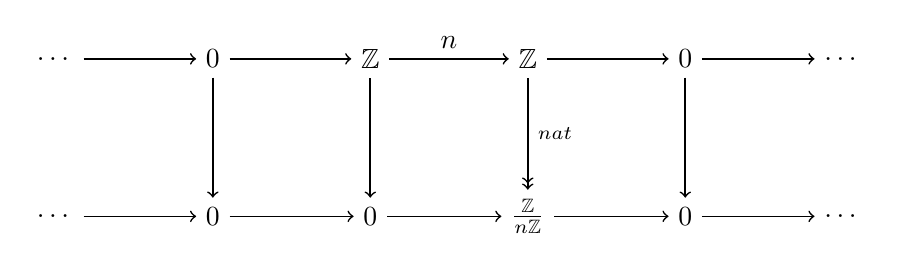
\begin{tikzpicture}[->,-latex, auto, main path/.style={->, semithick}, main node/.style={}]
\node	[main node]		(2) at (2,0)		{$\dots$};
\node	[main node]		(3) at (4,0)		{$0$};
\node [main node]		(4) at (6,0)		{$\bb{Z}$};
\node [main node]		(5) at (8,0)		{$\bb{Z}$};
\node	[main node]		(11) at (10,0)	{$0$};
\node [main node] 		(12) at (12,0)	{$\dots$};

\node	[main node]		(7) at (2,-2)		{$\dots$};
\node	[main node]		(8) at (4,-2)		{$0$};
\node [main node]		(9) at (6,-2)		{$0$};
\node [main node]		(10) at (8,-2)	{$\frac{\bb{Z}}{n\bb{Z}}$};
\node [main node]		(13) at (10,-2)	{$0$};
\node [main node]		(14) at (12, -2)	{$\dots$};

\draw (2) edge [main path] node [auto] {$$} (3);
\draw (3) edge [main path] node [auto] {$$} (4);
\draw (4) edge [main path] node [auto] {$n$} (5);
\draw (5) edge [main path] (11);
\draw (11) edge [main path] (12);

\draw (7) edge [main path] node [auto] {$$} (8);
\path (8) edge [main path] node [auto] {$$} (9);
\draw (9) edge [main path] node [auto, swap] {$$} (10);
\draw (10) edge [main path] (13);
\draw (13) edge [main path] (14);

\draw (3) edge [main path] node [auto] {$$} (8);
\draw (4) edge [main path] node [auto] {$$} (9);
\draw (5) edge [->>, semithick] node [auto] {$\scriptstyle{nat}$} (10);
\draw (11) edge [main path] (13);
\end{tikzpicture}
\end{equation*}
since the homologies are isomorphic at every $n$.
\end{eg}

\begin{mydef} \label{syzygiesdef}
Given a projective resolution $\mathbf{P}$ of $M$,
\begin{equation*}
\mathbf{P}:\quad \dots \xrightarrow{} P_n \xrightarrow{d_n} P_{n-1} \xrightarrow{} \dots \xrightarrow{} P_1 \xrightarrow{d_1} P_0 \xrightarrow{\epsilon} M \xrightarrow{} 0,
\end{equation*}
the \emph{syzygies} of $M$ are the modules $\Omega^nM=im(d_n:P_n \to P_{n-1}$ and $\Omega^0M=M$.\\
\end{mydef}

Note that here we used Crawley-Boevey's notation for the syzygies from \cite{CB1} rather than Rotman's in \cite{Rotman}. However, they are clearly the same definition as exactness of the projective resolution gives,
\begin{equation*}
K_n=ker(d_n:P_n \to P_{n-1}) = im(d_{n+1}:P_{n+1} \to P_n)=\Omega^{n+1}M,
\end{equation*}
and as the following remark demonstrates it is useful to recall this result:

\begin{lem} \label{syzygylem}
Defintion \ref{syzygiesdef} implies that there are exact sequences,
\begin{equation*}
0 \xrightarrow{} \Omega^{n+1}M \xrightarrow{} P_n \xrightarrow{} \Omega^nM \xrightarrow{} 0.
\end{equation*}
\end{lem}
\begin{proof}
Note that $\Omega^{n+1}M=im(d_{n+1}:P_{n+1} \to P_n)=ker(d_n:P_n \to P_{n-1})$ and $\Omega^nM=im(d_n:P_n \to P_{n-1})$.
\end{proof}

\begin{mydef}
If $M$ is an $R$-module, then an \emph{injective resolution} of $M$ is an exact sequence, 
\begin{equation*}
\mathbf{I}: \quad 0 \xrightarrow{}M \xrightarrow{\eta}I^0 \xrightarrow{d^0} I^1 \xrightarrow{d^1} I^2 \xrightarrow{} \dots,
\end{equation*}
where each $I^i$ is an injective module.
\end{mydef}

Since the defintion for a cosyzygy is not given in \cite{CB1} we turn to \cite{Rotman} for the following definition.

\begin{mydef}
Given an injective resolution,
\begin{equation*}
\mathbf{I}: \quad  0 \xrightarrow{} M \xrightarrow{\eta} I^0 \xrightarrow{d^0} I^1 \xrightarrow{} \dots \xrightarrow{} I^n \xrightarrow{d^n} I^{n+1} \xrightarrow{} \dots
\end{equation*}
the \emph{cosyzygies} of $M$ are the modules $\mho^n=coker(d^{n-1})$, for $n\geq 1$ and with $\mho^0M=coker(\eta)$.
\end{mydef}

\begin{thm} \label{comparisonthm} (Comparison Theorem)\\
Any map of modules $f:M \to M'$ can be lifted to a map of projective resolutions.
\begin{equation*}
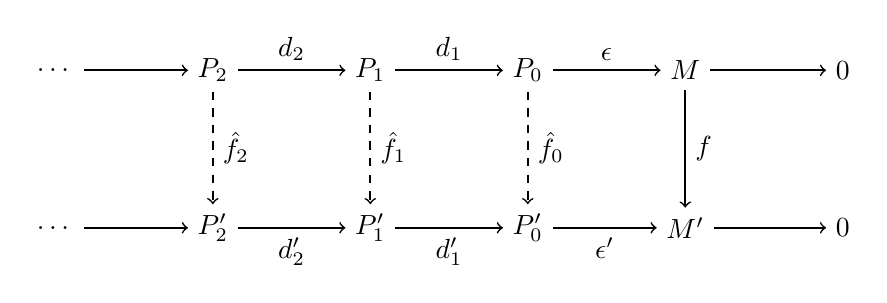
\begin{tikzpicture}[->,-latex, auto, main path/.style={->, semithick}, main node/.style={}]
\node	[main node]		(2) at (2,0)		{$\dots$};
\node	[main node]		(3) at (4,0)		{$P_2$};
\node [main node]		(4) at (6,0)		{$P_1$};
\node [main node]		(5) at (8,0)		{$P_0$};
\node	[main node]		(11) at (10,0)	{$M$};
\node [main node] 		(12) at (12,0)	{$0$};

\node	[main node]		(7) at (2,-2)		{$\dots$};
\node	[main node]		(8) at (4,-2)		{$P'_2$};
\node [main node]		(9) at (6,-2)		{$P'_1$};
\node [main node]		(10) at (8,-2)	{$P'_0$};
\node [main node]		(13) at (10,-2)	{$M'$};
\node [main node]		(14) at (12, -2)	{$0$};

\draw (2) edge [main path] node [auto] {$$} (3);
\draw (3) edge [main path] node [auto] {$d_2$} (4);
\draw (4) edge [main path] node [auto] {$d_1$} (5);
\draw (5) edge [main path] node [auto] {$\epsilon$} (11);
\draw (11) edge [main path] (12);

\draw (7) edge [main path] node [auto] {$$} (8);
\path (8) edge [main path] node [auto, swap] {$d'_2$} (9);
\draw (9) edge [main path] node [auto, swap] {$d'_1$} (10);
\draw (10) edge [main path] node [auto, swap] {$\epsilon'$} (13);
\draw (13) edge [main path] (14);

\draw (3) edge [dashed, ->, semithick] node [auto] {$\hat{f_2}$} (8);
\draw (4) edge [dashed, ->, semithick] node [auto] {$\hat{f_1}$} (9);
\draw (5) edge [dashed, ->, semithick] node [auto] {$\hat{f_0}$} (10);
\draw (11) edge [main path] node [auto] {$f$} (13);
\end{tikzpicture}
\end{equation*}
Moreover, any two such lifts are homotopic as chain maps $\mathbf{P}\to \mathbf{P'}$.
\end{thm}
\begin{proof}
Firstly, we show the existence of the lift. Consider the diagram:
\begin{equation} \label{comparisondiag}
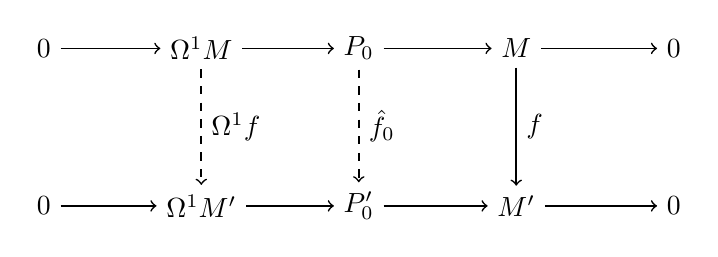
\begin{tikzpicture}[->,-latex, auto, main path/.style={->, semithick}, main node/.style={}]
\node	[main node]		(2) at (2,0)		{$0$};
\node	[main node]		(3) at (4,0)		{$\Omega^1M$};
\node [main node]		(4) at (6,0)		{$P_0$};
\node [main node]		(5) at (8,0)		{$M$};
\node	[main node]		(11) at (10,0)	{$0$};

\node	[main node]		(7) at (2,-2)		{$0$};
\node	[main node]		(8) at (4,-2)		{$\Omega^1M'$};
\node [main node]		(9) at (6,-2)		{$P'_0$};
\node [main node]		(10) at (8,-2)	{$M'$};
\node [main node]		(13) at (10,-2)	{$0$};

\draw (2) edge [main path] node [auto] {$$} (3);
\draw (3) edge [main path] node [auto] {$$} (4);
\draw (4) edge [main path] node [auto] {$$} (5);
\draw (5) edge [main path] (11);

\draw (7) edge [main path] node [auto] {$$} (8);
\path (8) edge [main path] node [auto] {$$} (9);
\draw (9) edge [main path] node [auto, swap] {$$} (10);
\draw (10) edge [main path] (13);

\draw (3) edge [dashed, ->, semithick] node [auto] {$\Omega^1f$} (8);
\draw (4) edge [dashed, ->, semithick] node [auto] {$\hat{f_0}$} (9);
\draw (5) edge [main path] node [auto] {$f$} (10);
\end{tikzpicture}
\end{equation}
Now as these are exact sequences by Lemma \ref{syzygylem}, the map $\epsilon': P_0' \to M'$ is surjective. Then since $P_0$ is projective we can lift the composite map $f\epsilon: P_0 \to M'$,
\begin{equation*}
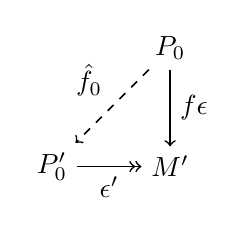
\begin{tikzpicture}[->,-latex, auto, main path/.style={->, semithick}, main node/.style={}]
\node [main node]		(1) at (1.5,1.5)		{$P_0$};
\node [main node]		(2) at (0,0)		{$P'_0$};
\node [main node]		(3) at (1.5,0)		{$M'$};

\draw (1) edge [main path] node [auto] {$f\epsilon$} (3);
\draw (1) edge [dashed, ->, semithick] node [auto, swap] {$\hat{f_0}$} (2);
\draw (2) edge [->>, semithick] node [auto, swap] {$\epsilon'$} (3);
\end{tikzpicture}
\end{equation*}
and so have a map $\hat{f_0}$ making the right hand square of \ref{comparisondiag} commute. Then by diagram chasing there is a map $\Omega^1f$ making the left hand square of \ref{comparisondiag} commute.\\
The same argument gets $\hat{f_1}$ and $\Omega^2f$.
\begin{equation*} 
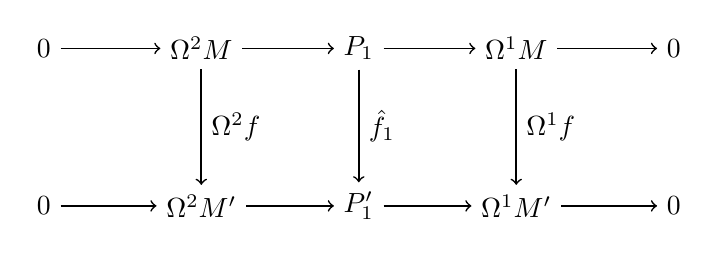
\begin{tikzpicture}[->,-latex, auto, main path/.style={->, semithick}, main node/.style={}]
\node	[main node]		(2) at (2,0)		{$0$};
\node	[main node]		(3) at (4,0)		{$\Omega^2M$};
\node [main node]		(4) at (6,0)		{$P_1$};
\node [main node]		(5) at (8,0)		{$\Omega^1M$};
\node	[main node]		(11) at (10,0)	{$0$};

\node	[main node]		(7) at (2,-2)		{$0$};
\node	[main node]		(8) at (4,-2)		{$\Omega^2M'$};
\node [main node]		(9) at (6,-2)		{$P'_1$};
\node [main node]		(10) at (8,-2)	{$\Omega^1M'$};
\node [main node]		(13) at (10,-2)	{$0$};

\draw (2) edge [main path] node [auto] {$$} (3);
\draw (3) edge [main path] node [auto] {$$} (4);
\draw (4) edge [main path] node [auto] {$$} (5);
\draw (5) edge [main path] (11);

\draw (7) edge [main path] node [auto] {$$} (8);
\path (8) edge [main path] node [auto] {$$} (9);
\draw (9) edge [main path] node [auto, swap] {$$} (10);
\draw (10) edge [main path] (13);

\draw (3) edge [main path] node [auto] {$\Omega^2f$} (8);
\draw (4) edge [main path] node [auto] {$\hat{f_1}$} (9);
\draw (5) edge [main path] node [auto] {$\Omega^1f$} (10);
\end{tikzpicture}
\end{equation*}
etc.\\
Finally, to show that any two lifts are homotopic it is equivalent to show that any lift of the zero map $M\to M'$ is homotopic to zero. Now,
\begin{equation*}
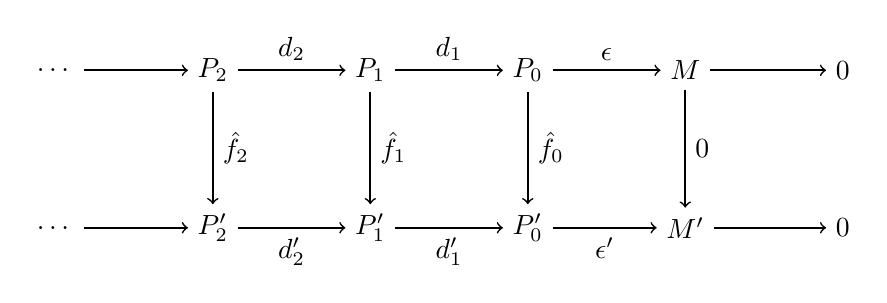
\begin{tikzpicture}[->,-latex, auto, main path/.style={->, semithick}, main node/.style={}]
\node	[main node]		(2) at (2,0)		{$\dots$};
\node	[main node]		(3) at (4,0)		{$P_2$};
\node [main node]		(4) at (6,0)		{$P_1$};
\node [main node]		(5) at (8,0)		{$P_0$};
\node	[main node]		(11) at (10,0)	{$M$};
\node [main node] 		(12) at (12,0)	{$0$};

\node	[main node]		(7) at (2,-2)		{$\dots$};
\node	[main node]		(8) at (4,-2)		{$P'_2$};
\node [main node]		(9) at (6,-2)		{$P'_1$};
\node [main node]		(10) at (8,-2)	{$P'_0$};
\node [main node]		(13) at (10,-2)	{$M'$};
\node [main node]		(14) at (12, -2)	{$0$};

\draw (2) edge [main path] node [auto] {$$} (3);
\draw (3) edge [main path] node [auto] {$d_2$} (4);
\draw (4) edge [main path] node [auto] {$d_1$} (5);
\draw (5) edge [main path] node [auto] {$\epsilon$} (11);
\draw (11) edge [main path] (12);

\draw (7) edge [main path] node [auto] {$$} (8);
\path (8) edge [main path] node [auto, swap] {$d'_2$} (9);
\draw (9) edge [main path] node [auto, swap] {$d'_1$} (10);
\draw (10) edge [main path] node [auto, swap] {$\epsilon'$} (13);
\draw (13) edge [main path] (14);

\draw (3) edge [main path] node [auto] {$\hat{f_2}$} (8);
\draw (4) edge [main path] node [auto] {$\hat{f_1}$} (9);
\draw (5) edge [main path] node [auto] {$\hat{f_0}$} (10);
\draw (11) edge [main path] node [auto] {$0$} (13);
\end{tikzpicture}
\end{equation*}
Then $\epsilon\hat{f_0}=0$ by commutativity, and so $\hat{f_0}$ has an image contained in $\Omega^1M'$. Now $d'_1: P'_1 \twoheadrightarrow \Omega^1M'$ is surjective and $P_0$ is projective so $\hat{f_0}$ lifts to a map $h_0:P_0 \to P'_1$.
\begin{equation*}
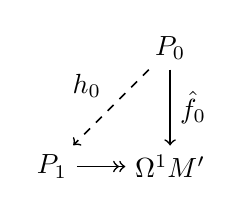
\begin{tikzpicture}[->,-latex, auto, main path/.style={->, semithick}, main node/.style={}]
\node [main node]		(1) at (1.5,1.5)		{$P_0$};
\node [main node]		(2) at (0,0)			{$P_1$};
\node [main node]		(3) at (1.5,0)		{$\Omega^1M'$};

\draw (1) edge [main path] node [auto] {$\hat{f_0}$} (3);
\draw (1) edge [dashed, ->, semithick] node [auto, swap] {$h_0$} (2);
\draw (2) edge [->>, semithick] node [auto, swap] {$$} (3);
\end{tikzpicture}
\end{equation*}
Thus $\hat{f_0}=d'_1h_0$.\\
Now suppose we have constructed $h_0, h_1, \dots, h_{n-1}$ with,
\begin{equation*}
\hat{f_i}=d_{i+1}h_i+h_{i-1}d_i, \text{ for } 0<i<n.
\end{equation*}
Then, 
\begin{align*}
d'_n(\hat{f_n}-h_{n-1}d_n)&=d'_n\hat{f_n} -d'_nh_{n-1}d_n, \\
&=\hat{f_{n-1}}d_n - d'_nh_{n-1}d_n, \text{ }(d'_n\hat{f_n}=\hat{f_{n-1}}d_n) \text{ by commutativity,}\\
&=(\hat{f_{n-1}}-d'_nh_{n-1})d_n.
\end{align*}
If $n=1$ then $(\hat{f_0}-d'_1h_0)d_1=0$ and if $n>1$ $(f_{n-1}-d'_nh_{n-1})d_n=(f_{n-1}-h_{n-2}d_{n-1})d_n$, so also zero. Thus $f_n-h_{n-1}d_n$ has image contained in $\Omega^{n+1}M'$. Thus it lifts to a map $h_n: P_n \to P'_{n+1}$.
\end{proof}

%%%%%%%%% NEED EXAMPLES!!!!!!!!!!!!!!!!!!!!!!!!!!!!!!

\begin{cor} \label{comparisoncor}
If $\mathbf{P}$ and $\mathbf{P'}$ are projective resolutions of $M$ then there is a homotopy equivalence $f: \mathbf{P} \to \mathbf{P'}$ such that the triangle, 
\begin{equation*}
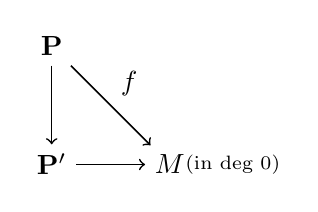
\begin{tikzpicture}[->,-latex, auto, main path/.style={->, semithick}, main node/.style={}]
\node [main node]		(1) at (0,1.5)		{$\mathbf{P}$};
\node [main node]		(2) at (0,0)			{$\mathbf{P'}$};
\node [main node]		(3) at (1.5,0)		{$M$};
\node [main node]		(4) at (2.3, 0)		{$\scriptstyle{(\text{in deg } 0)}$};

\draw (1) edge [main path] node [auto] {$f$} (3);
\draw (1) edge [main path] node [auto, swap] {$$} (2);
\draw (2) edge [main path] node [auto, swap] {$$} (3);
\end{tikzpicture}
\end{equation*}
commutes. Moreover, $f$ is unique up to homotopy.
\end{cor}
\begin{proof}
The identity map $id_M: M \to M$ lifts to chain maps $f: \mathbf{P} \to \mathbf{P'}$ and $g:\mathbf{P'} \to \mathbf{P}$. Now $gf: \mathbf{P} \to \mathbf{P}$ is a lift of the identity map $id_M$, so it is homotopic to $id_{\mathbf{P}}$. Similarly, $fg: \mathbf{P'} \to \mathbf{P'}$ is homotopic to $id_{\mathbf{P'}}$.\\
The uniqueness of $f$ up to homotopy is part of the Comparison Theorem (Thm \ref{comparisonthm}).
\end{proof}

This last part of the section gives a small introduction to projective covers which will be used to define the Auslander-Reiten translate in Chapter 4.
\begin{mydef}
A submodule $N$ of a module $M$ is \emph{surperfluous} if, whenever $L\subseteq M$ is a submodule with $L+S=M$, then $L=M$.
\end{mydef}

\begin{mydef}
A \emph{projective cover} of a module $M$ is an ordered pair $(P,\epsilon)$ where $P$ is projective and $\epsilon: P \to M$ is a surjective map with $ker\epsilon$ a superfluous submodule of $P$.
\end{mydef}

\begin{lem}
Let $(P,\epsilon)$ be a projective cover of a module $M$. If $P'$ is projective and $\psi: P' \to M$ is surjective, then any lifting $\phi: P' \to P$ is surjective.
\begin{equation*}
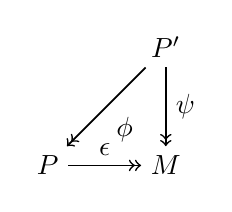
\begin{tikzpicture}[->,-latex, auto, main path/.style={->>, semithick}, main node/.style={}]
\node	[main node]		(2) at (0,0)			{$P$};
\node	[main node]		(3) at (1.5,0)		{$M$};
\node [main node]		(4) at (1.5,1.5)		{$P'$};

\draw (2) edge [main path] node [auto] {$\epsilon$} (3);
\draw (4) edge [main path] node [auto] {$\psi$} (3);
\draw (4) edge [main path] node [auto] {$\phi$} (2);
\end{tikzpicture}
\end{equation*}
\end{lem}
\begin{proof}
See \cite{Rotman}
\end{proof}

\begin{rem}
In \cite{Vale} we have the results that if $A$ is a finite dimensional $k$-algebra, then for each left module $M$ there exists projective cover. Furthermore, if $(P, \epsilon)$ and $(P', \epsilon')$ are projective covers of $M$ then $P\cong P'$.
\end{rem}

%%%%%%%%%%%%%%%%%%%%%%%%%%%%%%%%%%%%%%%%%%%%%%%%%%%%%%%
%%%%%%%%%%%%%%%%%%		EXT		%%%%%%%%%%%%%%%%%%%%%%%%%%
%%%%%%%%%%%%%%%%%%%%%%%%%%%%%%%%%%%%%%%%%%%%%%%%%%%%%%%

\section{Ext}

The following section contains theory on the right-derived functor $Ext$, however, in an effort to steer clear of category theory, this report will define $Ext$ as Crawley-Boevey does in \cite{CB1}. If the reader is interested in exploring category theory and $Ext$ as a functor they are directed to start with Appendix A of \cite{Weibel} which introduces category theory language and then look at the derived functors sections in both \cite{Weibel} and \cite{Rotman}. This section will follow \cite{CB1} closely as it explores $Ext$ theory without the need of category theory, with some  additional results from \cite{Weibel}. As such, the reader is advised that, unless otherwise stated, the results of this section come from \cite{CB1}, with only minor details added where it is felt they aid the reader's understanding.

\begin{mydef}
If $M$ and $N$ are $R$-modules then $Ext^n(M, N)$, or more precisely $Ext^n_R(M, N)$, is defined as follows:
\begin{itemize}
\item Choose a projective resolution $\mathbf{P}$ of $M$.
\item Set $Ext^n(M, N)=H^n(\mathbf{P}, N)$.
\end{itemize}
Thus if, 
\begin{equation*}
\dots \xrightarrow{}P_2 \xrightarrow{} P_1 \xrightarrow{} P_0 \xrightarrow{}M\xrightarrow{}0,
\end{equation*}
 is the projective resolution, then $Ext^n(M, N)$ is the cohomology in degree $n$ of the cochain complex,
\begin{equation*}
0\xrightarrow{} Hom(P_0, N) \xrightarrow{} Hom(P_1, N) \xrightarrow{} Hom(P_2, N)\xrightarrow{} \dots
\end{equation*}
\end{mydef}
 
\begin{rem}
Note that this definition does not depend on the choice of projective resolution. If $\mathbf{P'}$ is another projective resolution there there is a homotopy equivalence $f: \mathbf{P} \to \mathbf{P'}$ by Corollary \ref{comparisoncor}. This gives a homotopy equivalence of cochain complexes $f^{\ast}: Hom(\mathbf{P'}, N) \to Hom(P, N)$. Proposition \ref{homequivisomprop} says this is a quasi-isomorphism and so induces isomorphisms on the cohomology $H^n(\mathbf{P'}, N) \to H^n(\mathbf{P}, N)$.  Moreover, the homotopy equivalence $f$ is unique up to homotopy, so the cochain map is unique up to homotopy. Thus the map $H^n(\mathbf{P'}, N) \to H^n(\mathbf{P}, N)$ is uniquely determined.
\end{rem}

\begin{prop}
\begin{description}
\item [(i)] If $\theta: N \to N'$ is a map there is a natural map $ Ext^n(M, N) \to Ext^n(M, N')$.
\item[(ii)] If $\phi: M'' \to M$ is a map there is a natural map $ Ext^n(M, N) \to Ext^n(M'', N)$.
\end{description}
\end{prop}
\begin{proof}
\begin{description}
\item [(i)] As $\mathbf{P}$ is a projective resolution of $M$, $\theta: N \to N'$ induces a chain map $Hom(\mathbf{P}, N) \to Hom(\mathbf{P'}, N)$.
\item [(ii)] $\phi: M'' \to M$ lifts to a chain map $\mathbf{P''} \to \mathbf{P}$ of projective resolutions unique up to homotopy (Thm \ref{comparisonthm}) and so induces a cochain map $Hom(\mathbf{P}, N) \to Hom(\mathbf{P''}, N)$ unique up to homotopy, giving unique maps on $Ext^n$.
\end{description}
\end{proof}

\begin{prop}
\begin{description}
\item [(i)] $Ext^n(M, N\oplus N') \cong Ext^n(M, N) \oplus Ext^n(M, N')$.
\item [(ii)] $Ext^n(M\oplus M', N) \cong Ext^n(M, N) \oplus Ext^n(M', N)$.
\end{description}
\end{prop}
\begin{proof}
\begin{description}
\item [(i)] If $\mathbf{P}$ is a projective resolution of $M$ then $Hom(\mathbf{P}, N\oplus N')\cong Hom(\mathbf{P}, N) \oplus Hom(\mathbf{P}, N')$.
\item [(ii)] If $\mathbf{P'}$ is a projective resolution of $M'$ then $\mathbf{P} \oplus \mathbf{P'}$ is a projective resolution of $M\oplus M'$ and $Hom(\mathbf{P} \oplus \mathbf{P'}, N) \cong Hom(\mathbf{P}, N) \oplus Hom(\mathbf{P'}, N)$.
\end{description}
\end{proof}

\begin{lem}
\begin{equation*}
Ext^n(M, N) \cong 
\begin{cases}
0& n<0,\\
Hom(M,N) & n=0,\\
coker(Hom(P_{n-1}, N) \xrightarrow{\iota^{\ast}_{n-1}} Hom(\Omega^nM, N) & n>0,\\
\end{cases}
\end{equation*}
where $0\xrightarrow{} \Omega^nM \xrightarrow{\iota_n} P_{n-1} \xrightarrow{}\Omega^{n-1}M\xrightarrow{}0$.
\end{lem}
\begin{proof}
$n<0$: The claim is clear as $Hom(\mathbf{P}, N)$ is a non-negative cochain complex.\\
$n\geq 0$: By definition,
\begin{equation*}
Ext^n(M,N)=H^n(\mathbf{P},N)=\frac{ker(d^{\ast}_{n+1}:Hom(P_{n}, N) \to Hom(P_{n+1}, N))}{im(d^{\ast}_n:Hom(P_{n-1}, N) \to Hom(P_{n}, N))}.
\end{equation*}
Thus, 
\begin{align*}
Ext^n(M,N) &=\frac{ker(d^{\ast}_{n+1}:Hom(P_{n}, N) \to Hom(P_{n+1}, N))}{im(d^{\ast}_n:Hom(P_{n-1}, N) \to Hom(P_{n}, N))}, \\
& \cong \frac{codomain(\gamma: Hom(P_{n-1}, N) \to ker(d^{\ast}_{n+1}))}{im(\gamma:Hom(P_{n-1}, N) \to ker(d^{\ast}_{n+1}))},\\
& \cong coker(\gamma: Hom(Hom(P_{n-1}, N) \to ker(d^{\ast}_{n+1}))).
\end{align*}
Now there is an exact sequence, 
\begin{equation*}
P_{n+1} \xrightarrow{d_{n+1}} P_n \xrightarrow{d_n} \Omega^nM \xrightarrow{}0,
\end{equation*}
which then induces the exact sequence,
\begin{equation*}
0 \xrightarrow{} Hom(\Omega^nM, N) \twoheadrightarrow Hom(P_n, N) \xrightarrow{d^{\ast}_{n+1} } Hom(P_{n+1}, N),
\end{equation*}
and so, $ker(d^{\ast}_{n+1}) \cong im(Hom(\Omega^nM, N))\twoheadrightarrow Hom(P_n, N)) \cong Hom(\Omega^nM, N)$.\\ 
Note that if we let $P_{-1}=0$ and $\iota_0:M \to 0$ then at $n=0$ we have,
\begin{align*}
coker(Hom(P_{-1}, N) \xrightarrow{\iota^{\ast}_0} Hom(\Omega^0M, N))&=coker(Hom(0, N) \xrightarrow{\iota^{\ast}_0} Hom(M, N), \\
&\cong Hom(M,N).
\end{align*}
\end{proof}

\begin{prop} \label{longexactHom(X,-)prop}
If $X$ is a module then for any short exact sequence $0\xrightarrow{}L\xrightarrow{}M\xrightarrow{}N\xrightarrow{}0$ you get a long exact sequence, 
\begin{align*}
0 \xrightarrow{}& Hom(X,L) \xrightarrow{} Hom(X, M) \xrightarrow{} Hom(X, N) \xrightarrow{} \\
\xrightarrow{} & Ext^1(X,L) \xrightarrow{} Ext^1(X,M) \xrightarrow{} Ext^1(X,N) \xrightarrow{}\\
\xrightarrow{} & Ext^2(X,L) \xrightarrow{} \dots
\end{align*}
It is called the long exact sequence for $Hom(X,-)$.
\end{prop}
\begin{proof}
This is the long exact sequence in cohomology for the chain complex $\mathbf{P}$, a projective resolution of $X$. (Corollary \ref{longexactseqcor}).
\end{proof}

\begin{lem} \label{Ext=0lem}
$Ext^n(M,N)=0$ for $n>0$ if either:
\begin{description}
\item [(i)] $M$ is projective, or, 
\item [(ii)] $N$ is injective.
\end{description}
\end{lem}
\begin{proof}
\begin{description}
\item [(i)] If $M$ is projective you can use the projective resolution,
\begin{equation*}
\dots \xrightarrow{} 0 \xrightarrow{} 0 \xrightarrow{} M \xrightarrow{} M \xrightarrow{} 0.
\end{equation*}
\item [(ii)] If $N$ is injective then the exact sequence,
\begin{equation*}
0\xrightarrow{} \Omega^nM \xrightarrow{\iota_n} P_{n-1} \xrightarrow{} \Omega^{n-1}M \xrightarrow{} 0,
\end{equation*}
gives an exact sequence, 
\begin{equation*}
0 \xrightarrow{} Hom(\Omega^{n-1}M, N) \xrightarrow{} Hom(P_{n-1}, N) \xrightarrow{} Hom(\Omega^nM, N) \xrightarrow{}0,
\end{equation*}
so $coker(\iota^{\ast}_n)=0$.
\end{description}
\end{proof}

\begin{prop}
If $0\xrightarrow{}N \xrightarrow{} I^0 \xrightarrow{} I^1 \xrightarrow{} \dots $ is an injective resolution of $N$ then you can complute $Ext^n(M,N)$ as the cohomology of the cochain complex $Hom(M,\mathbf{I})$,
\begin{equation*}
0 \xrightarrow{} Hom(M,I^0) \xrightarrow{} Hom(M, I^1) \xrightarrow{} Hom(M,I^2) \xrightarrow{} \dots
\end{equation*}
\end{prop}
\begin{proof}
Firstly, we break the injective resolution into short exact sequences,
\begin{equation*}
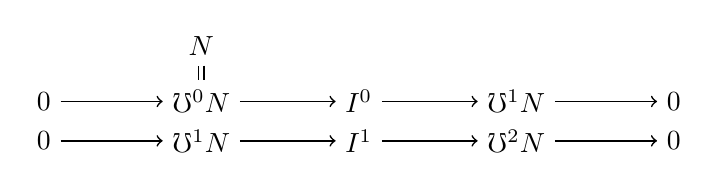
\begin{tikzpicture}[->,-latex, auto, main path/.style={->, semithick}, main node/.style={}]
\node	[main node]		(2) at (2,0)		{$0$};
\node	[main node]		(3) at (4,0)		{$\mho^0N$};
\node [main node]		(4) at (6,0)		{$I^0$};
\node [main node]		(5) at (8,0)		{$\mho^1N$};
\node	[main node]		(11) at (10,0)	{$0$};
\node [main node] 		(12) at (4, 0.7) 	{$N$};

\node	[main node]		(7) at (2,-0.5)	{$0$};
\node	[main node]		(8) at (4,-0.5)	{$\mho^1N$};
\node [main node]		(9) at (6,-0.5)	{$I^1$};
\node [main node]		(10) at (8,-0.5)	{$\mho^2N$};
\node [main node]		(13) at (10,-0.5)	{$0$};

\draw (2) edge [main path] node [auto] {$$} (3);
\draw (3) edge [main path] node [auto] {$$} (4);
\draw (4) edge [main path] node [auto] {$$} (5);
\draw (5) edge [main path] node [auto] {$$} (11);

\draw (7) edge [main path] node [auto] {$$} (8);
\path (8) edge [main path] node [auto, swap] {$$} (9);
\draw (9) edge [main path] node [auto, swap] {$$} (10);
\draw (10) edge [main path] node [auto, swap] {$$} (13);

\draw (12) edge [-, double, double distance=1.5pt, semithick] (3);
\end{tikzpicture}
\end{equation*}
and so on. You then get a long exact sequence,
\begin{align*}
0 &\xrightarrow{} Hom(M, \mho^iN) \xrightarrow{} Hom(M,I^i) \xrightarrow{} Hom(M, \mho^{i+1}N)\xrightarrow{}\\
&\xrightarrow{} Ext^1(M,\mho^iN) \twoheadrightarrow 0 \hookrightarrow Ext^1(M, \mho^{i+1}N)\xrightarrow{}\\
&\xrightarrow{} Ext^2(M, \mho^iN) \twoheadrightarrow 0 \hookrightarrow \dots
\end{align*}
Thus,
\begin{align*}
Ext^n(M,N) &\cong Ext^{n-1}(M, \mho^iN) \cong \dots \cong Ext^1(M, \mho^{n-1}N), \text{ by dimension shifting,}\\
&\cong coker(Hom(M,I^{n-1}) \xrightarrow{} Hom(M,\mho^nN)).
\end{align*}
Now, $0\xrightarrow{} \mho^nN \xrightarrow{}I^n \xrightarrow{} I^{n+1}$ is exact, so,
\begin{equation*}
0 \xrightarrow{} Hom(M, \mho^nN) \xrightarrow{} Hom(M,I^n) \xrightarrow{} Hom(M,I^{n+1}),
\end{equation*}
is exact. The claim follows. %%%%% What claim and what does it do???
\end{proof}

\begin{prop}
If $Y$ is a module for any short exact sequence $0\xrightarrow{} L \xrightarrow{} M \xrightarrow{}N \xrightarrow{}0$ you have a long exact sequence,
\begin{align*}
0 &\xrightarrow{} Hom(N,Y) \xrightarrow{} Hom(M,Y) \xrightarrow{} Hom(L,Y) \xrightarrow{}\\
&\xrightarrow{} Ext^1(N,Y) \xrightarrow{} Ext^1(M,Y) \xrightarrow{} Ext^1(L,Y) \xrightarrow{}\\
&\xrightarrow{} Ext^2(N,Y) \xrightarrow{} \dots
\end{align*}
This is called the long exact sequence of $Hom(-,Y)$.
\end{prop}
\begin{proof}
Let $\mathbf{I}$ be a injective resolution of $Y$ then the maps $f:L \to M$ and $g:M \to N$ induce maps of cochain complexes,
\begin{equation*}
Hom(N,\mathbf{I}) \xrightarrow{} Hom(M,\mathbf{I}) \xrightarrow{} Hom(L,\mathbf{I}).
\end{equation*}
This is an exact sequence of cochain complexes since $I^n$ is injective for all $n$. Now use the long exact sequence in cohomology from Remark \ref{longexactseqcochainrem}.
\end{proof}

\begin{mydef}
For any short exact sequence $\mathbf{E}: 0 \xrightarrow{} L \xrightarrow{} M \xrightarrow{} N \xrightarrow{} 0$ we define an element $\mathbf{\hat{E}}\in Ext^1(N,L)$ as follows. The long exact sequence for $Hom(N,-)$ (see Proposition \ref{longexactHom(X,-)prop}) gives a map $\delta: Hom(N,N) \to Ext^1(N,L)$, the connecting map, and $\mathbf{\hat{E}}$ is the image of $id_N$ under this map.
\end{mydef}

\begin{lem} \label{alphabetalem}
Fix a projective resolution of $N$, giving exact sequences,
\begin{equation*}
0 \xrightarrow{} \Omega^1N \xrightarrow{\iota} P_0 \xrightarrow{\epsilon} N \xrightarrow{}0,
\end{equation*}
and,
\begin{equation*}
Hom(P_0,L) \xrightarrow{\iota^{\ast}} Hom(\Omega^1N,L) \xrightarrow{} Ext^1(N,L) \xrightarrow{}0.
\end{equation*}
If $\mathbf{E}: 0 \xrightarrow{}L \xrightarrow{} M \xrightarrow{}L\xrightarrow{}0$ is a short exact sequence then you can find maps $\alpha, \beta$ giving a commutative diagram,
\begin{equation*}
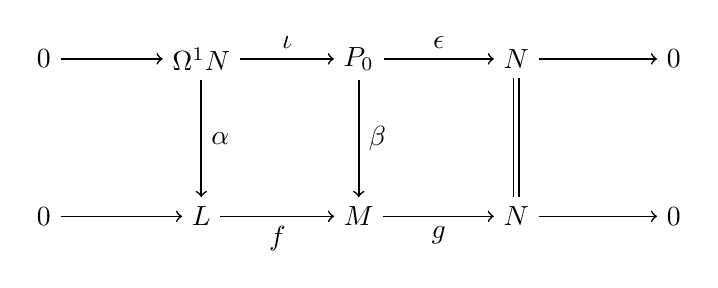
\begin{tikzpicture}[->,-latex, auto, main path/.style={->, semithick}, main node/.style={}]
\node	[main node]		(2) at (2,0)		{$0$};
\node	[main node]		(3) at (4,0)		{$\Omega^1N$};
\node [main node]		(4) at (6,0)		{$P_0$};
\node [main node]		(5) at (8,0)		{$N$};
\node	[main node]		(11) at (10,0)	{$0$};

\node	[main node]		(7) at (2,-2)		{$0$};
\node	[main node]		(8) at (4,-2)		{$L$};
\node [main node]		(9) at (6,-2)		{$M$};
\node [main node]		(10) at (8,-2)	{$N$};
\node [main node]		(13) at (10,-2)	{$0$};

\draw (2) edge [main path] node [auto] {$$} (3);
\draw (3) edge [main path] node [auto] {$\iota$} (4);
\draw (4) edge [main path] node [auto] {$\epsilon$} (5);
\draw (5) edge [main path] node [auto] {$$} (11);

\draw (7) edge [main path] node [auto] {$$} (8);
\path (8) edge [main path] node [auto, swap] {$f$} (9);
\draw (9) edge [main path] node [auto, swap] {$g$} (10);
\draw (10) edge [main path] node [auto, swap] {$$} (13);

\draw (3) edge [main path] node [auto] {$\alpha$} (8);
\draw (4) edge [main path] node [auto] {$\beta$} (9);
\draw (5) edge [-, double, semithick, double distance=1.5pt] (10);
\end{tikzpicture}
\end{equation*}
Moreover, for any such commutative diagram the image of $\alpha$ in $Ext^1(N,L)$ is equal to $\mathbf{\hat{E}}$.
\end{lem}
\begin{proof}
Existence of $\alpha, \beta$: Since $P_0$ is projective and $g: M\to N$ is surjective (short exact sequence), by the definition of projective modules we can lift the map $P_0 \to N$ to a map $\beta$ such that,
\begin{equation*}
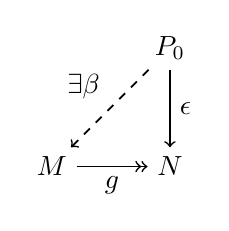
\begin{tikzpicture}[->,-latex, auto, main path/.style={->, semithick}, main node/.style={}]
\node [main node]		(1) at (0,0)		{$M$};
\node [main node]		(2) at (1.5,0)	{$N$};
\node [main node]		(3) at (1.5, 1.5)	{$P_0$};

\draw (1) edge [->>, semithick] node [auto, swap] {$g$} (2);
\draw (3) edge [main path] node [auto] {$\epsilon$} (2);
\draw (3) edge [->, dashed, semithick] node [auto, swap] {$\exists \beta$} (1);
\end{tikzpicture}
\end{equation*}
Then $\alpha$ exists by diagram chasing.
As we have a projective resolution of $N$, we can apply $Hom(N,-)$ to $\mathbf{E}$ to obtain (Propn. \ref{longexactHom(X,-)prop}),
\begin{equation*}
0\xrightarrow{} Hom(N,L) \xrightarrow{} Hom(N,M) \xrightarrow{} Hom(N,N) \xrightarrow{\delta} Ext^1(N,L) \xrightarrow{} \dots
\end{equation*}
and so find the connecting map $\delta: Hom(N,N) \to Ext^1(N,L)$. Note that this is the connecting map in cohomology for the exact sequence of cochain complexes,
\begin{equation*}
0 \xrightarrow{} Hom(\mathbf{P},L) \xrightarrow{} Hom(\mathbf{P},M) \xrightarrow{} Hom(\mathbf{P},N) \xrightarrow{} 0.
\end{equation*}
This begins,
\begin{equation*}
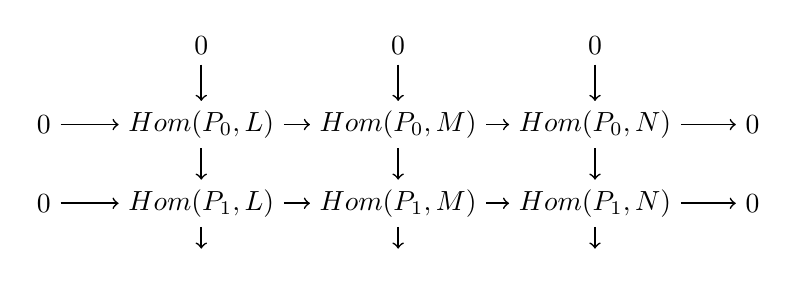
\begin{tikzpicture}[->,-latex, auto, main path/.style={->, semithick}, main node/.style={}]
\node	[main node]		(2) at (0,0)		{$0$};
\node	[main node]		(3) at (2,0)		{$Hom(P_0, L)$};
\node [main node]		(4) at (4.5,0)	{$Hom(P_0,M)$};
\node [main node]		(5) at (7,0)		{$Hom(P_0, N)$};
\node	[main node]		(11) at (9,0)		{$0$};

\node	[main node]		(7) at (0,-1)		{$0$};
\node	[main node]		(8) at (2,-1)		{$Hom(P_1, L)$};
\node [main node]		(9) at (4.5,-1)	{$Hom(P_1, M)$};
\node [main node]		(10) at (7,-1)		{$Hom(P_1, N)$};
\node [main node]		(13) at (9,-1)	{$0$};

\node [main node]		(-1) at (2,1)		{$0$};
\node [main node]		(-2) at (4.5,1)	{$0$};
\node [main node]		(-3) at (7,1)		{$0$};

\node [main node]		(-4) at (2,-1.7)	{$$};
\node [main node]		(-5) at (4.5,-1.7)	{$$};
\node [main node]		(-6) at (7,-1.7)	{$$};

\draw (2) edge [main path] node [auto] {$$} (3);
\draw (3) edge [main path] node [auto] {$$} (4);
\draw (4) edge [main path] node [auto] {$$} (5);
\draw (5) edge [main path] node [auto] {$$} (11);

\draw (7) edge [main path] node [auto] {$$} (8);
\path (8) edge [main path] node [auto, swap] {$$} (9);
\draw (9) edge [main path] node [auto, swap] {$$} (10);
\draw (10) edge [main path] node [auto, swap] {$$} (13);

\draw (3) edge [main path] node [auto] {$$} (8);
\draw (4) edge [main path] node [auto] {$$} (9);
\draw (5) edge [main path] (10);

\draw(-1) edge [main path] (3);
\draw (-2) edge [main path] (4);
\draw (-3) edge [main path] (5);

\draw(8) edge [main path] (-4);
\draw (9) edge [main path] (-5);
\draw (10) edge [main path] (-6);
\end{tikzpicture}
\end{equation*}
Then $Hom(N,N)\cong Ext^0(N,N)=H^0(\mathbf{P}, N)$ and, 
\begin{align*}
H^0(\mathbf{P}, N) &=\text{cohomology at } Hom(P_0,N),\\
&=\frac{ker(Hom(P_0, N) \to Hom(P_1, N))}{im(0 \to Hom(P_0, N))},\\
&=ker(Hom(P_0, N) \to Hom(P_1, N)),
\end{align*}
 and so we have $id_N$ corresponding to $\overline{\epsilon}$. From earlier $\beta$ is a lifting of $\epsilon$ in $Hom(P_1, M)$. Let $\gamma$ be the corresponding element in $Hom(P_1, L)$. Then the diagram,
\begin{equation*}
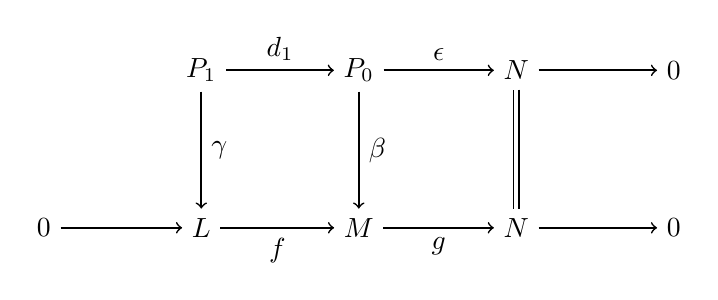
\begin{tikzpicture}[->,-latex, auto, main path/.style={->, semithick}, main node/.style={}]
\node	[main node]		(3) at (4,0)		{$P_1$};
\node [main node]		(4) at (6,0)		{$P_0$};
\node [main node]		(5) at (8,0)		{$N$};
\node	[main node]		(11) at (10,0)	{$0$};

\node	[main node]		(7) at (2,-2)		{$0$};
\node	[main node]		(8) at (4,-2)		{$L$};
\node [main node]		(9) at (6,-2)		{$M$};
\node [main node]		(10) at (8,-2)	{$N$};
\node [main node]		(13) at (10,-2)	{$0$};

\draw (3) edge [main path] node [auto] {$d_1$} (4);
\draw (4) edge [main path] node [auto] {$\epsilon$} (5);
\draw (5) edge [main path] node [auto] {$$} (11);

\draw (7) edge [main path] node [auto] {$$} (8);
\path (8) edge [main path] node [auto, swap] {$f$} (9);
\draw (9) edge [main path] node [auto, swap] {$g$} (10);
\draw (10) edge [main path] node [auto, swap] {$$} (13);

\draw (3) edge [main path]  node [auto] {$\gamma$} (8);
\draw (4) edge [main path] node [auto] {$\beta$} (9);
\draw (5) edge [-, double, semithick, double distance=1.5pt] (10);
\end{tikzpicture}
\end{equation*}
commutes. However, the composition,
\begin{equation*}
\begin{tikzpicture}[->,-latex, auto, main path/.style={->, semithick}, main node/.style={}]
\node [main node]		(2) at (2,0)		{$P_2$};
\node	[main node]		(3) at (4,0)		{$P_1$};

\node	[main node]		(8) at (4,-2)		{$L$};
\node [main node]		(9) at (6,-2)		{$M$};

\draw (2) edge [main path] node [auto] {$d_2$} (3);
\path (8) edge [main path] node [auto, swap] {$f$} (9);
\draw (3) edge [main path]  node [auto] {$\gamma$} (8);
\end{tikzpicture}
\end{equation*}
is equal to,
\begin{equation*}
\begin{tikzpicture}[->,-latex, auto, main path/.style={->, semithick}, main node/.style={}]
\node [main node]		(2) at (2,0)		{$P_2$};
\node	[main node]		(3) at (4,0)		{$P_1$};
\node [main node]		(4) at (6,0)		{$P_0$};

\node [main node]		(9) at (6,-2)		{$M$};

\draw (3) edge [main path] node [auto] {$d_1$} (4);
\draw (2) edge [main path] node [auto] {$d_2$} (3);
\draw (4) edge [main path] node [auto] {$\beta$} (9);
\end{tikzpicture}
\end{equation*}
and so is zero as $d_1d_2=0$.Hence, since $f:L \to M$ is injective, the composition $\gamma d_2: P_2 \to L$ is zero. Thus $\gamma$ induces a map $\sfrac{P_1}{Im(d_2)} \to L$, i.e. $\alpha: \Omega^1N \to L$.
\end{proof}

\begin{thm} 
There exists a bijection $\Uptheta$,
\begin{equation*}
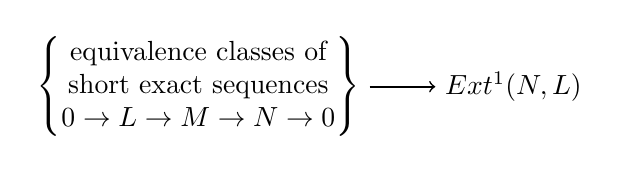
\begin{tikzpicture}[->,-latex, auto, main path/.style={->, semithick}, main node/.style={}]
\node [main node] 	(1) at (0,0)		{$\left\{\mytab{equivalence classes of\\ short exact sequences\\ $0\to L \to M \to N \to 0$}\right\}$};
\node [main node]			(2) at (4,0)		{$Ext^1(N,L)$};

\draw (1) edge  [->, semithick] (2);
\end{tikzpicture}
\end{equation*}
\end{thm}
\begin{proof}
Firstly we want to show that $\Uptheta$ is well defined:\\
Consider two equivalent exact sequences $\mathbf{E}, \mathbf{E'}$, they become the bottom two rows of the diagram, 
\begin{equation*}
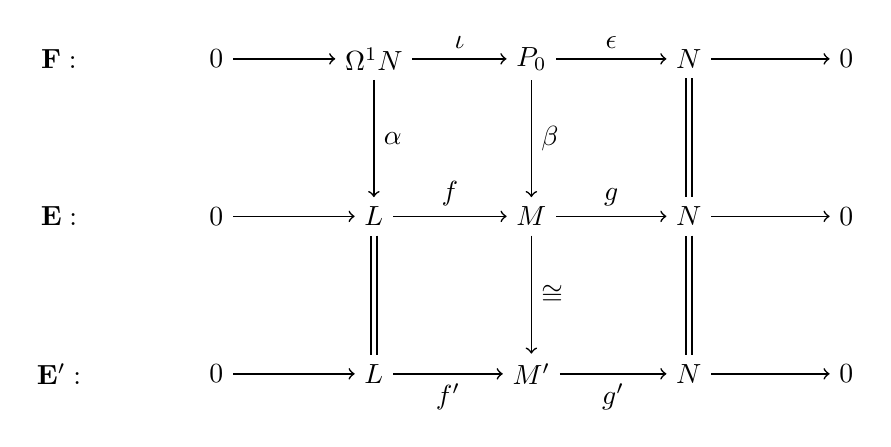
\begin{tikzpicture}[->,-latex, auto, main path/.style={->, semithick}, main node/.style={}]
\node [main node]		(1) at (0,0)		{$\mathbf{E}:$};
\node	[main node]		(2) at (2,0)		{$0$};
\node	[main node]		(3) at (4,0)		{$L$};
\node [main node]		(4) at (6,0)		{$M$};
\node [main node]		(5) at (8,0)		{$N$};
\node	[main node]		(11) at (10,0)	{$0$};

\node [main node] 		(6) at (0,-2)		{$\mathbf{E'}:$};
\node	[main node]		(7) at (2,-2)		{$0$};
\node	[main node]		(8) at (4,-2)		{$L$};
\node [main node]		(9) at (6,-2)		{$M'$};
\node [main node]		(10) at (8,-2)	{$N$};
\node [main node]		(13) at (10,-2)	{$0$};

\node [main node] 		(14) at (0,2)		{$\mathbf{F}:$};
\node	[main node]		(15) at (2,2)		{$0$};
\node	[main node]		(16) at (4,2)		{$\Omega^1N$};
\node [main node]		(17) at (6,2)		{$P_0$};
\node [main node]		(18) at (8,2)		{$N$};
\node [main node]		(19) at (10,2)	{$0$};

\draw (2) edge [main path] node [auto] {$$} (3);
\draw (3) edge [main path] node [auto] {$f$} (4);
\draw (4) edge [main path] node [auto] {$g$} (5);
\draw (5) edge [main path] node [auto] {$$} (11);

\draw (7) edge [main path] node [auto] {$$} (8);
\path (8) edge [main path] node [auto, swap] {$f'$} (9);
\draw (9) edge [main path] node [auto, swap] {$g'$} (10);
\draw (10) edge [main path] node [auto, swap] {$$} (13);

\draw (15) edge [main path] node [auto] {$$} (16);
\path (16) edge [main path] node [auto] {$\iota$} (17);
\draw (17) edge [main path] node [auto] {$\epsilon$} (18);
\draw (18) edge [main path] node [auto, swap] {$$} (19);

\draw (3) edge [-,double, semithick, double distance=1.5pt] (8);
\draw (4) edge [main path] node [auto] {$\cong$} (9);
\draw (5) edge [-, double, semithick, double distance=1.5pt] (10);

\draw (16) edge [main path] node [auto] {$\alpha$} (3);
\draw (17) edge [main path] node [auto] {$\beta$} (4);
\draw (18) edge [-, double, semithick, double distance=1.5pt] (5);
\end{tikzpicture}
\end{equation*}
where $\theta$ is an isomorphism. So $\mathbf{E}$ and $\mathbf{E'}$ give rise to the same map $\gamma: P_1 \to L$ (or $\alpha: \Omega^1 \to L$) by Lemma \ref{alphabetalem} and so $\hat{E}=\hat{E'}$.\\
Secondly, we need to show that $\Uptheta$ is surjective:\\
Set $g\in Ext^1(N,L)$. Then this corresponds to some $\alpha \in Hom(\Omega^1N, L)$ as in the long exact sequence, 
\begin{equation*}
0 \xrightarrow{} Hom(N,L) \xrightarrow{} Hom(P_0, L) \xrightarrow{} Hom(\Omega^1N, L) \xrightarrow{\delta} Ext^1(N,L) \xrightarrow{}0\xrightarrow{} \dots
\end{equation*}
$\delta$ is surjective. So we have, 
\begin{equation*}
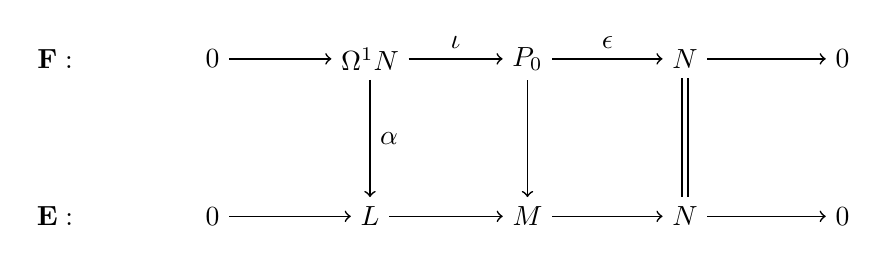
\begin{tikzpicture}[->,-latex, auto, main path/.style={->, semithick}, main node/.style={}]
\node [main node]		(1) at (0,0)		{$\mathbf{E}:$};
\node	[main node]		(2) at (2,0)		{$0$};
\node	[main node]		(3) at (4,0)		{$L$};
\node [main node]		(4) at (6,0)		{$M$};
\node [main node]		(5) at (8,0)		{$N$};
\node	[main node]		(11) at (10,0)	{$0$};

\node [main node] 		(14) at (0,2)		{$\mathbf{F}:$};
\node	[main node]		(15) at (2,2)		{$0$};
\node	[main node]		(16) at (4,2)		{$\Omega^1N$};
\node [main node]		(17) at (6,2)		{$P_0$};
\node [main node]		(18) at (8,2)		{$N$};
\node [main node]		(19) at (10,2)	{$0$};

\draw (2) edge [main path] node [auto] {$$} (3);
\draw (3) edge [main path] node [auto] {$$} (4);
\draw (4) edge [main path] node [auto] {$$} (5);
\draw (5) edge [main path] node [auto] {$$} (11);

\draw (15) edge [main path] node [auto] {$$} (16);
\path (16) edge [main path] node [auto] {$\iota$} (17);
\draw (17) edge [main path] node [auto] {$\epsilon$} (18);
\draw (18) edge [main path] node [auto, swap] {$$} (19);

\draw (16) edge [main path] node [auto] {$\alpha$} (3);
\draw (17) edge [main path] node [auto] {$$} (4);
\draw (18) edge [-, double, semithick, double distance=1.5pt] (5);
\end{tikzpicture}
\end{equation*}
where $\mathbf{E}$ is the pushout of $\mathbf{F}$ along $\alpha$. By construction, $\mathbf{E}$ is an exact sequence, unique up to equivalence, so any element of $Ext^1(N,L)$ is the image of an equivalence class of short exact sequences.\\
Finally, we prove that $\Uptheta$ is injective:
If two short exact sequences $\mathbf{E}, \mathbf{E'}$ give the same element $\hat{E}\in Ext^1(N,L)$ then we have diagrams, 
\begin{equation*}
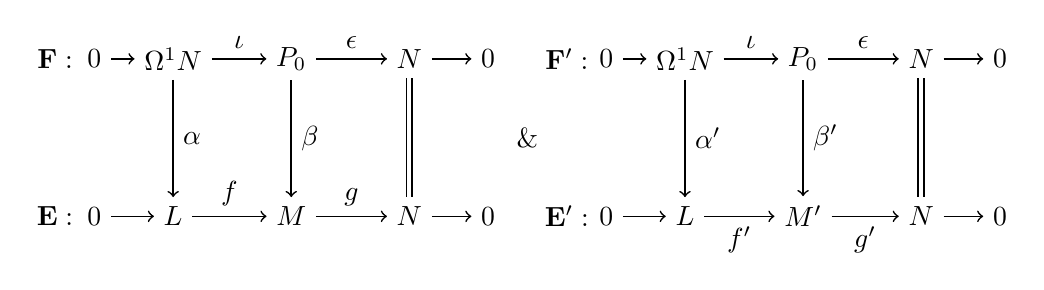
\begin{tikzpicture}[->,-latex, auto, main path/.style={->, semithick}, main node/.style={}]
\node [main node]		(1) at (1,0)		{$\mathbf{E}:$};
\node	[main node]		(2) at (1.5,0)	{$0$};
\node	[main node]		(3) at (2.5,0)	{$L$};
\node [main node]		(4) at (4,0)		{$M$};
\node [main node]		(5) at (5.5,0)	{$N$};
\node	[main node]		(11) at (6.5,0)	{$0$};

\node [main node] 		(6) at (7.5,0)		{$\mathbf{E'}:$};
\node	[main node]		(7) at (8,0)		{$0$};
\node	[main node]		(8) at (9,0)		{$L$};
\node [main node]		(9) at (10.5,0)	{$M'$};
\node [main node]		(10) at (12,0)	{$N$};
\node [main node]		(13) at (13,0)	{$0$};

\node [main node] 		(14) at (1,2)		{$\mathbf{F}:$};
\node	[main node]		(15) at (1.5,2)	{$0$};
\node	[main node]		(16) at (2.5,2)	{$\Omega^1N$};
\node [main node]		(17) at (4,2)		{$P_0$};
\node [main node]		(18) at (5.5,2)	{$N$};
\node [main node]		(19) at (6.5,2)	{$0$};

\node [main node] 		(20) at (7.5,2)	{$\mathbf{F'}:$};
\node	[main node]		(21) at (8,2)		{$0$};
\node	[main node]		(22) at (9,2)		{$\Omega^1N$};
\node [main node]		(23) at (10.5,2)	{$P_0$};
\node [main node]		(24) at (12,2)	{$N$};
\node [main node]		(25) at (13,2)	{$0$};

\node [main node]		(26) at (7,1)		{\&};

\draw (2) edge [main path] node [auto] {$$} (3);
\draw (3) edge [main path] node [auto] {$f$} (4);
\draw (4) edge [main path] node [auto] {$g$} (5);
\draw (5) edge [main path] node [auto] {$$} (11);

\draw (7) edge [main path] node [auto] {$$} (8);
\path (8) edge [main path] node [auto, swap] {$f'$} (9);
\draw (9) edge [main path] node [auto, swap] {$g'$} (10);
\draw (10) edge [main path] node [auto, swap] {$$} (13);

\draw (15) edge [main path] node [auto] {$$} (16);
\path (16) edge [main path] node [auto] {$\iota$} (17);
\draw (17) edge [main path] node [auto] {$\epsilon$} (18);
\draw (18) edge [main path] node [auto, swap] {$$} (19);

\draw (21) edge [main path] node [auto] {$$} (22);
\path (22) edge [main path] node [auto] {$\iota$} (23);
\draw (23) edge [main path] node [auto] {$\epsilon$} (24);
\draw (24) edge [main path] node [auto, swap] {$$} (25);

\draw (16) edge [main path] node [auto] {$\alpha$} (3);
\draw (17) edge [main path] node [auto] {$\beta$} (4);
\draw (18) edge [-, double, semithick, double distance=1.5pt] (5);

\draw (22) edge [main path] node [auto] {$\alpha'$} (8);
\draw (23) edge [main path] node [auto] {$\beta'$} (9);
\draw (24) edge [-, double, semithick, double distance=1.5pt] (10);
\end{tikzpicture}
\end{equation*}
with $\alpha'-\alpha\in im(Hom(P_0,L) \xrightarrow{\iota^{\ast}}Hom(\Omega^1N,L))$ from the long exact sequence, 
\begin{equation*}
0 \xrightarrow{} Hom(N,L) \xrightarrow{} Hom(P_0,L) \xrightarrow{\iota^{\ast}} Hom(\Omega^1N, L) \xrightarrow{\delta} Ext^1(N,L) \xrightarrow{} 0 \xrightarrow{} \dots
\end{equation*}
and so $im(\iota^{\ast})=ker(\delta)$ by exactness and so we can map $\alpha'-\alpha \mapsto \hat{E} - \hat{E}=0$. Now say $\alpha'-\alpha=\phi \circ \iota$ with $\phi: P_0 \to L$, then,
\begin{equation*}
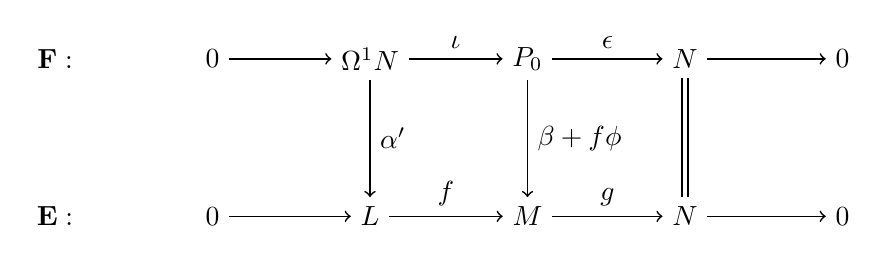
\begin{tikzpicture}[->,-latex, auto, main path/.style={->, semithick}, main node/.style={}]
\node [main node]		(1) at (0,0)		{$\mathbf{E}:$};
\node	[main node]		(2) at (2,0)		{$0$};
\node	[main node]		(3) at (4,0)		{$L$};
\node [main node]		(4) at (6,0)		{$M$};
\node [main node]		(5) at (8,0)		{$N$};
\node	[main node]		(11) at (10,0)	{$0$};

\node [main node] 		(14) at (0,2)		{$\mathbf{F}:$};
\node	[main node]		(15) at (2,2)		{$0$};
\node	[main node]		(16) at (4,2)		{$\Omega^1N$};
\node [main node]		(17) at (6,2)		{$P_0$};
\node [main node]		(18) at (8,2)		{$N$};
\node [main node]		(19) at (10,2)	{$0$};

\draw (2) edge [main path] node [auto] {$$} (3);
\draw (3) edge [main path] node [auto] {$f$} (4);
\draw (4) edge [main path] node [auto] {$g$} (5);
\draw (5) edge [main path] node [auto] {$$} (11);

\draw (15) edge [main path] node [auto] {$$} (16);
\path (16) edge [main path] node [auto] {$\iota$} (17);
\draw (17) edge [main path] node [auto] {$\epsilon$} (18);
\draw (18) edge [main path] node [auto, swap] {$$} (19);

\draw (16) edge [main path] node [auto] {$\alpha'$} (3);
\draw (17) edge [main path] node [auto] {$\beta + f\phi$} (4);
\draw (18) edge [-, double, semithick, double distance=1.5pt] (5);
\end{tikzpicture}
\end{equation*}
Hence by the uniqueness of pushouts, $\mathbf{E}$ and $\mathbf{E'}$ are equivalent.
\end{proof}

%Need Examples!!

\begin{prop}
The split exact sequences of an equivalence class of extensions of $N$ by $L$ correspond to the zero element of $Ext^1(N,L)$.
\end{prop}
\begin{proof}
Lemma \ref{splitequivlem} gives that any two split extensions of $N$ by $L$ are equivalent, and so in the same equivalence class. Note that if $\mathbf{E}: \quad0 \xrightarrow{} L \xrightarrow{}M \xrightarrow{}N \xrightarrow{} 0$ splits then as $M \cong L\oplus N$ (Cor. \ref{MLNcor}), $\mathbf{E}$ is equivalent to $0 \xrightarrow{}L \xrightarrow{} L \oplus N \xrightarrow{} N \xrightarrow{} 0$. Relabel this exact sequence $\mathbf{E}$. Let $\xrightarrow{} P_1 \xrightarrow{}P_0 \xrightarrow{} N \xrightarrow{}0$ be the projective resolution of $N$. Then, by Lemma \ref{alphabetalem} we have a commutative diagram,
\begin{equation*}
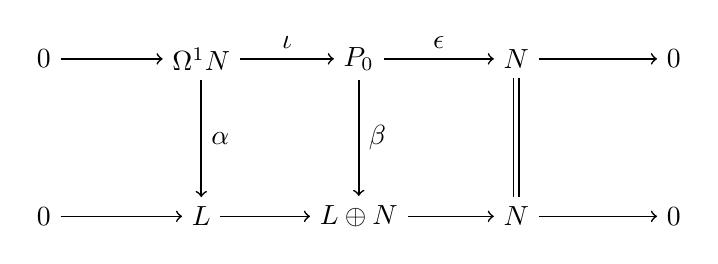
\begin{tikzpicture}[->,-latex, auto, main path/.style={->, semithick}, main node/.style={}]
\node	[main node]		(2) at (0,0)		{$0$};
\node	[main node]		(3) at (2,0)		{$\Omega^1N$};
\node [main node]		(4) at (4,0)		{$P_0$};
\node [main node]		(5) at (6,0)		{$N$};
\node	[main node]		(11) at (8,0)		{$0$};

\node	[main node]		(7) at (0,-2)		{$0$};
\node	[main node]		(8) at (2,-2)		{$L$};
\node [main node]		(9) at (4,-2)		{$L\oplus N$};
\node [main node]		(10) at (6,-2)	{$N$};
\node [main node]		(13) at (8,-2)	{$0$};

\draw (2) edge [main path]  (3);
\draw (3) edge [main path]  node [auto] {$\iota$} (4);
\draw (4) edge [main path]  node [auto] {$\epsilon$} (5);
\draw (5) edge [main path] (11);

\draw (7) edge [main path] node [auto] {$$} (8);
\path (8) edge [main path] node [auto, swap] {$$} (9);
\draw (9) edge [main path] node [auto, swap] {$$} (10);
\draw (10) edge [main path] node [auto, swap] {$$} (13);

\draw (3) edge [main path] node [auto] {$\alpha$} (8);
\draw (4) edge [main path] node [auto] {$\beta$} (9);
\draw (5) edge [-, double, semithick, double distance=1.5pt] (10);
\end{tikzpicture}
\end{equation*}
and applying $Hom(-,L)$ to the top row gives the long exact sequence, 
\begin{equation*}
0 \xrightarrow{} Hom(N,L) \xrightarrow{} Hom(P_0, L) \xrightarrow{} Hom(\Omega^1N, L) \xrightarrow{\delta} Ext^1(N,L) \xrightarrow{} 0 \xrightarrow{} \dots
\end{equation*}
with $\delta(\alpha)=\hat{E}$. However, $\alpha=0$ by diagram chasing, and so $\hat{E}=0$.
\end{proof}

This result is interesting as it means, as Rotman points out in \cite{Rotman}, the non-zero elements of $Ext^1(N,L)$ describe nonsplit extensions of $N$ by $L$.

\begin{mydef}
The \emph{projective dimension} of a module $M$ is the smallest $n\in \bb{Z}$ such that there is a finite projective resolution of $M$,
\begin{equation*}
0 \xrightarrow{} P_n \xrightarrow{} \dots \xrightarrow{} P_1 \xrightarrow{} P_0 \xrightarrow{} M \xrightarrow{} 0.
\end{equation*}
It is denoted $pd(M)=n$. If no such finite projective resolution exists, then $pd(M)=\infty$.
\end{mydef}

\begin{mydef}
The \emph{global dimension} of the ring $R$ is the maximum of the projective dimensions of its modules.
\end{mydef}

\begin{prop}
Let $M$ be a module and $n\geq0$. The following are equivalent:
\begin{description}
\item [(i)] $pd(M)=n$.
\item [(ii)] $Ext^{n+1}(M,N)=0$ for all modules $N$.
\end{description}
\end{prop}
\begin{proof}
(i) $\Rightarrow$ (ii): This is trivial, as if $P_{n+1}=0$ then the cohomology of the long exact sequence will also be equal to zero.\\
(ii) $\Rightarrow$ (i): If $\mathbf{P}$ is a projective resolution then there is an exact sequence,
\begin{equation*}
0 \xrightarrow{} \Omega^nM \xrightarrow{\iota} P_{n-1} \xrightarrow{} \dots \xrightarrow{} P_0 \xrightarrow{} M \xrightarrow{} 0,
\end{equation*}
and so it suffices to prove $\Omega^nM$ is projective as then this exact sequence is the required projective resolution. This condition is satisfied if $Ext(\Omega^nM,N)=0$ for all $N$. The exact sequence, 
\begin{equation*}
0 \xrightarrow{} \Omega^nM \xrightarrow{} P_{n-1} \xrightarrow{} \Omega^{n-1}M \xrightarrow{} 0,
\end{equation*}
gives a long exact sequence which includes,
\begin{equation*}
\dots \xrightarrow{} Ext^1(P_{n-1},N) \xrightarrow{} Ext^1(\Omega^nM,N) \xrightarrow{} Ext^2(\Omega^{n-1}M,N) \xrightarrow{} Ext^2(P_{n-1},N) \xrightarrow{} \dots
\end{equation*}
However, $P_{n-1}$ is projective so $Ext^i(P_{n-1},N)=0$ for all $i$ and so we have,
\begin{equation*}
\dots \xrightarrow{} 0 \xrightarrow{} Ext^1(\Omega^nM,N) \xrightarrow{} Ext^2(\Omega^{n-1}M,N) \xrightarrow{} 0 \xrightarrow{} \dots
\end{equation*}
Hence, $Ext^1(\Omega^nM, N) \cong Ext^2(\Omega^{n-1}M,N)$. Then by dimension shifting we get, 
\begin{align*}
Ext^2(\Omega^{n-1}M,N) \cong Ext^3(\Omega^{n-2}M,N) \cong \dots \cong Ext^{n+1}(\Omega^0M,N)&= Ext^{n+1}(M,N), \\
&=0.
\end{align*}
\end{proof}








%%%%%%%%%%%%%%%%%%%%%%%%%%%%%%%%%%%%%%%%%%%%%%%%%%%%%%%
%%%%%%%%%%%%%%		Representation of Quivers 	%%%%%%%%%%%%%%%%%%%%%%%
%%%%%%%%%%%%%%%%%%%%%%%%%%%%%%%%%%%%%%%%%%%%%%%%%%%%%%%



\chapter{Representation of Quivers}

%%%%%%%%%%%%%%%%%%%%%%%%%%%%%%%%%%%%%%%%%%%%%%%%%%%%%%
%%%%%%%%%%%%%%		Quivers and Path Algebras	%%%%%%%%%%%%%%%%%%%%%%%
%%%%%%%%%%%%%%%%%%%%%%%%%%%%%%%%%%%%%%%%%%%%%%%%%%%%%%%

\section{Quivers and Path Algebras}

\begin{mydef}
A \emph{quiver} is defined as the tuple of sets and functions, $\mathbf{Q}=(Q_0\text{, }Q_1\text{, }s\text{, }t: Q_1 \to Q_0)$ such that:
\begin{itemize}
\item $Q_0$ is the set of vertices, which we will set to be the finite set $\{1, 2, \dots, n\}$.
\item $Q_1$ is the set of arrows, which we will also set to be finite.
\item Functions $s, t$ such that an arrow $\rho \in Q_1$ \emph{starts} at the vertex $s(\rho)\in Q_0$ and \emph{terminates} at the vertex $t(\rho)\in Q_0$, i.e. $\rho: s(\rho) \to t(\rho)$.
\end{itemize}
\end{mydef}

\begin{eg} \label{ininquivereg}
A quiver $Q=(Q_0, Q_1, s, t:Q_1 \to Q_0)$ where $Q_0=\{1, 2, 3, 4\}$, $Q_1=\{\alpha, \beta\}$, and $s, t$ are defined such that;
\begin{align*}
s:& Q_1 \to Q_0\text{,\quad} \alpha \mapsto 1\text{, } \beta \mapsto 2\text{, } \gamma \mapsto 4\\
t:& Q_1 \to Q_0\text{,\quad} \alpha \mapsto 2\text{, } \beta \mapsto 3\text{, } \gamma \mapsto 3,
\end{align*}
looks like,
\begin{equation*}
\mathbf{Q}: \qquad
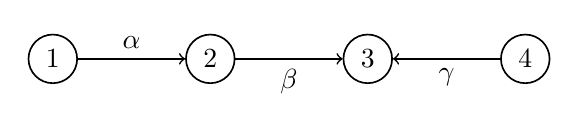
\begin{tikzpicture}[->,-latex, auto, every path/.style={->, semithick}, main node/.style={draw, circle}]
\node	[main node]		(1) at (0,0)		{1};
\node	[main node]		(2) at (2,0)		{2};
\node	[main node]		(3) at (4,0)		{3};
\node [main node]		(4) at (6,0)		{4};

\draw (1) edge node [auto] {$\alpha$} (2);
\draw (2) edge node [auto, swap] {$\beta$} (3);
\draw (4) edge node [auto] {$\gamma$} (3);
\end{tikzpicture}
\end{equation*}
\end{eg}

\begin{mydef}
A \emph{non-trivial path}, $p$, in the quiver $Q$,  is a sequence of arrows $\rho_1, \dots, \rho_n$ which satisfies $t(\rho_{i+1})=s(\rho_i)$ for all $1\leq i <n$. Pictorially, 
\begin{equation*}
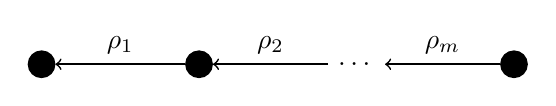
\begin{tikzpicture}[->,-latex, auto, every path/.style={->, semithick}, main node/.style={draw, circle, fill}]
\node	[main node]		(1) at (0,0)		{};
\node	[main node]		(2) at (2,0)		{};
\node				(3) at (4,0)		{\dots};
\node [main node]		(4) at (6,0)		{};

\draw (2) edge node [auto, swap] {$\rho_1$} (1);
\draw (3) edge node [auto, swap] {$\rho_2$} (2);
\draw (4) edge node [auto, swap] {$\rho_m$} (3);
\end{tikzpicture}
\end{equation*}
 The starting and terminatinating vertex of a path $p$, $s(\rho_1)$ and $t(\rho_1)$, are denoted $s(p)$ and $t(p)$, respectively.
\end{mydef}

\begin{note}
In this report the arrows in a path will be ordered the same way as the composition of functions, as in \cite{CB2}, however, be aware that other publications may order the arrows the opposite way.
\end{note}

\begin{mydef}
The \emph{trivial path} is the path which contains no arrows, i.e. it is a single vertex, and is denoted $e_i$ where the vertex is $i$.
\end{mydef}

\begin{eg} \label{ininpatheg}
The paths of the quiver in Example \ref{ininquivereg} are:
\begin{equation*}
p_1=e_1, \quad p_2=e_2, \quad p_3=e_3, \quad p_4=e_4, \quad p_5=\alpha, \quad p_6=\beta, \quad p_7=\gamma, \quad p_8=\beta\alpha.
\end{equation*}
However, $\gamma\beta\alpha$ is not a path because $t(\beta)=3\neq s(\gamma)=2$.
\end{eg}

\begin{mydef}
A \emph{path algebra} $kQ$ is the $k$-alegbra which has a basis all the paths in $Q$, and the product of two paths $p,q$ is defined as,
\begin{equation*}
pq=\begin{cases}
\text{obvious composition} & \text{if } t(q)=s(p),\\
0 & \text{otherwise.}
\end{cases}
\end{equation*}
This multiplication is assosciative.
\end{mydef}

\begin{eg}
If we once again use the quiver $Q$ from Example \ref{ininquivereg}, then, from Example \ref{ininpatheg}, we know the basis of the path algebra $kQ$ will be,
\begin{equation*}
\{e_1, e_2, e_3, e_4,\alpha, \beta, \gamma, \beta\alpha\}.
\end{equation*}
The product of $\beta$ and $\alpha$ is $\beta\alpha$, but the product of $\alpha$ and $\beta$ is zero, and the product of $e_2$ and $\alpha$ is just $\alpha$.
\end{eg}

\begin{eg}
If $Q$ is the following quiver,
\begin{equation*}
\mathbf{Q}: \qquad
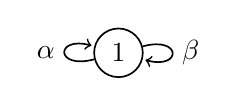
\begin{tikzpicture}[->,-latex, auto, every path/.style={->, semithick}, main node/.style={draw, circle}]
\node	[main node]		(1) at (0,0)		{1};

\draw (1) edge[loop left] node [auto] {$\alpha$} (1);
\draw (1) edge [loop right] node [auto] {$\beta$} (1);
\end{tikzpicture}
\end{equation*}
forms the path algebra $kQ\cong k<X, Y$, the free, assosciative algebra on two letters. In fact, if we have a quiver with a single vertex and $n$ loops, then this can be associated with the free, assosciated algebra on $n$ letters.
\end{eg}

\begin{rem}
Recall that $UT_n(k)$ is the algebra of $n\times n$ upper triangular matrices over a field $k$. Similarly, $LT_n(k)$ is the algebra of $n\times n$ lower triangular matrices over a field $k$.
\end{rem}

\begin{eg} \label{UTpathalgebraeg}
If we have the quiver,
\begin{equation*}
\mathbf{Q}: \qquad
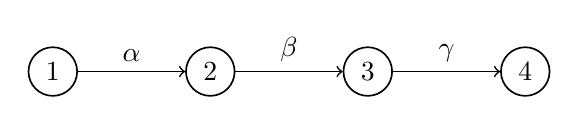
\begin{tikzpicture}[->,-latex, auto, every path/.style={->, semithick}, main node/.style={draw, circle}]
\node	[main node]		(1) at (0,0)		{1};
\node [main node]		(2) at (2,0)		{2};
\node [main node]		(3) at (4,0)		{3};
\node [main node]		(4) at (6,0)		{4};

\draw (1) edge node [auto] {$\alpha$} (2);
\draw (2) edge node [auto] {$\beta$} (3);
\draw (3) edge node [auto] {$\gamma$} (4);
\end{tikzpicture}
\end{equation*}
the the path algebra, $kQ \cong UT_4(k)$ by the isomorphism,
\begin{multline*}
\lambda_1e_1+\lambda_2e_2+\lambda_3e_3+\lambda_4e_4+\lambda_5\alpha+\\
\lambda_6\beta+\lambda_7\gamma+\lambda_8\beta\alpha+\lambda_9\gamma\beta\alpha+\lambda_{10}\gamma\beta
\mapsto
\begin{pmatrix*}
\lambda_4 & \lambda_7 & \lambda_{10} & \lambda_9 \\
0 & \lambda_3 & \lambda_6 & \lambda_{8}\\
0 & 0 & \lambda_2 & \lambda_5 \\
0 & 0 & 0 & \lambda_1
\end{pmatrix*}
\end{multline*}
Generally, a quiver of the form,
\begin{equation*}
\mathbf{Q'}: \qquad
\begin{tikzpicture}[->,-latex, auto, every path/.style={->, semithick}, main node/.style={draw, circle}]
\node	[main node]		(1) at (0,0)		{1};
\node [main node]		(2) at (2,0)		{2};
\node []			(3) at (4,0)		{$\dots$};
\node [main node]		(4) at (6,0)		{n};

\draw (1) edge node [auto] {$\alpha$} (2);
\draw (2) edge node [auto] {$\beta$} (3);
\draw (3) edge node [auto] {$\gamma$} (4);
\end{tikzpicture}
\end{equation*}
induces a path alegbra $kQ' \cong UT_n(k)$ for any $n$.
\end{eg}

\begin{eg}
In fact, we find that if $Q$ is the same quiver as above in Example \ref{UTpathalgebraeg}, then $kQ \cong LT_4(k)$ as well, through the isomorphism,
\begin{multline*}
\lambda_1e_1+\lambda_2e_2+\lambda_3e_3+\lambda_4e_4+\lambda_5\alpha+\\
\lambda_6\beta+\lambda_7\gamma+\lambda_8\beta\alpha+\lambda_9\gamma\beta\alpha+\lambda_{10}\gamma\beta
\mapsto
\begin{pmatrix*}
\lambda_1 & 0 & 0 & 0\\
\lambda_5 & \lambda_2 & 0 & 0\\
\lambda_8 & \lambda_6 & \lambda_3 & 0\\
\lambda_9 & \lambda_{10} & \lambda_7 & \lambda_4
\end{pmatrix*}.
\end{multline*}
Once again, this extends to the general case that, $kQ' \cong LT_n(k)$.
\end{eg}

\begin{eg} \label{pathalgebramatrixeg}
In a more general case, as long as there is only one path between any two vertices, we can identify $kQ$ with the following subalgebra of $M_n(k)$,
\begin{equation*}
\{M \in M_n(k): M_ij=0 \text{ if there is no path from } j \text{ to }i\}.
\end{equation*}
For instance, if we have the quiver,
\begin{equation*}
\mathbf{Q}: \qquad
\begin{tikzpicture}[->,-latex, auto, every path/.style={->, semithick}, main node/.style={draw, circle}]
\node	[main node]		(1) at (0,0)		{1};
\node [main node]		(2) at (2,0)		{2};
\node [main node]		(3) at (4,0)		{3};
\node [main node]		(4) at (6,-1)		{4};
\node [main node]		(5) at (6,1)		{5};
\node [main node]		(6) at (8, 1)		{6};

\draw (1) edge node [auto] {$\alpha$} (2);
\draw (2) edge node [auto] {$\beta$} (3);
\draw (3) edge node [auto] {$\gamma$} (4);
\draw (5) edge node [auto, swap] {$\delta$} (3);
\draw (5) edge node [auto] {$\epsilon$} (6);
\end{tikzpicture}
\end{equation*}
the we can see that the path algebra $kQ$ is isomorphic to the subalgebra with matrices of the form,
\begin{equation*}
\begin{pmatrix*}
1 & 0 & 0 & 0 & 0 & 0 \\
1 & 1 & 0 & 0 & 0 & 0 \\
1 & 1 & 1 & 0 & 1 & 0 \\
1 & 1 & 1 & 1 & 1 & 0 \\
0 & 0 & 0 & 0 & 1 & 0 \\
0 & 0 & 0 & 0 & 1 & 1
\end{pmatrix*}
\end{equation*}
\end{eg}

\begin{rem}
Note that the idea here has some parallels to similar results for directed graphs in graph theory.
\end{rem}

The following results about the idempotents of path alegebras are from \cite{CB2}, however, we have either given a proof or expanded upon the one given. For the following results we set $A=kQ$ and the $e_i$ are the trivial paths of $Q$.

\begin{mydef} 
Let $\Lambda$ be an algebra.
\begin{itemize}
\item An element $e\in \Lambda$ is said to be \emph{idempotent} if $ee=e$.
\item Idempotent elements $e,e'\in \Lambda$ are said to be \emph{orthogonal} if $ee'=e'e=0$.
\item A nonzero idempotent element $e\in \Lambda$ is said to be \emph{primitive} if whenever $e=e'+e''$, with $e',e''\in \Lambda$ orthogonal indempotents then either $e'=0$ or $e''=0$.
\end{itemize}
\end{mydef}

\begin{lem} \label{identitylem}
The $e_i$ are orthogonal idempotents in $A$. Thus $\sum_{i=1}^{n}{e_i}=1_{A}$.
\end{lem}
\begin{proof}
Obviously, $e_ie_j=0$ when$i\neq j$ because $t(e_j)\neq s(e_i)$ because they are the trivial paths at different vertices, $i$ and $j$. Similarly, if we have the product $e_ie_i$ then the composition makes sense here because $t(e_i)=s(e_i)$, but the composition is just $e_i$ becuase if we travel along the trivial path $e_i$ twice, then this is just the same as travelling the trivial path. \\
If we have some path $p$ of the quiver, then bear in mind that,
\begin{equation*}
e_ip=
\begin{cases}
e_ip=p & \text{if } i=t(p),\\
0 & \text{otherwise.}
\end{cases}
\end{equation*}
Hence, the sum of the trivial paths acting on our path $p$ becomes, 
\begin{equation*}
\big(\sum^{n}_{i=1}{e_i}\big)p=(e_1+e_2+\dots +e_n)p=e_ip=p=1_Ap,
\end{equation*}
because only one of the $e_i$ in the sum will satisfy $i=t(p)$ and all the rest will give zero. Similary, we can show that $p\big(\sum^{n}_{i=1}{e_i}\big)=p1_A$.
\end{proof}

\begin{lem} \label{idempotentspaceslem}
The spaces $Ae_i$ and $e_jA$ have as bases all the paths starting at $i$ and all the paths terminating at $j$, respectively. Moreover, the space $e_jAe_i$ has as a basis the paths that start at $i$ and terminate at $j$.
\end{lem}
\begin{proof}
Set $i\in Q_0$. Let $P$ be the set of all paths in $Q$ which start at the vertex $i$. Note that as $Q$ may have oriented cycles, $P$ is not necessarily finite dimensional. We have $P \subset Ae_i$ since if $q \in P$ then $p=pe_i\in Ae_i$. Next want to show that $P$ is linearly independent and spans $Ae_i$. Firstly, recall from the definition of a path algebra that the set of all paths in $Q$ forms a basis for $A$. Hence, all the paths in $Q$ are linearly independent and moreover so are all the paths in $P$. Now suppose we have an element $ae_i\in Ae_i$ then $a\in A$ and so $a=\sum_{j} \lambda_ip_i$, however, we can rewrite this $a=\sum_r\mu_rq_r + \sum_s \mu'_sq_s$ where $q_r\in P$ and the $q'_s$ are paths in $Q$ not starting at vertex $i$. Then, $ae_i=\sum_r\mu_rq_r$ and so $P$ spans $Ae_i$. Thus, we can see that the basis of $Ae_i$ must be all the paths starting at $i$. Similarly, as $e_jA$ is a subspace of $A$ snd so following a similar argument we can see that its basis must be all the paths terminating at $j$. The result for $e_jAe_i$ follows from these as it simply the intersection of the two spaces.
\end{proof}

\begin{lem}
$A=\oplus^n_{i=1}Ae_i$, so each $Ae_i$ is a projective left $A$-module.
\end{lem}
\begin{proof}
Firstly, let us convince ourselves that $A$ is indeed equal to $\oplus^n_{i=1}Ae_i$. Recall from Lemma \ref{identitylem} that $1_A=\sum^n_{i=1}e_i$ and it is also clear that $Ae_i \bigcap Ae_j=\{0\}$ for all $i\neq j$. Hence, $A=Ae_1\oplus \dots \oplus Ae_n$.\\
From Lemma \ref{idempotentspaceslem} we know that for each $i$, the basis of $Ae_i$ are all the paths starting at $i$ and so $\oplus^n_{i=1}Ae_i$ must have as a basis all the paths starting at every vertex in $Q$, hence all the paths in $Q$. Thus $A=\oplus^n_{i=1}Ae_i$. Also, each $Ae_i$ is obviously a left $A$-module with the action defined as multiplication by $e_i$. Hence, each $Ae_i$ is a projective, left $A$-module.
\end{proof}

\begin{rem}
Similarly, $A=\oplus_{i=1}^ne_jA$, so each $e_jA$ is a projective, right $A$-module.
\end{rem}

\begin{lem} \label{idempotenthomlem}
If $X$ is a left $A$-module, then $Hom_A(Ae_i,X)\cong e_iX$.
\end{lem}
\begin{proof}
Want to show that there are some maps $f$ and $g$,
\begin{equation*}
f: Hom_A(Ae_i, X) \to e_iX \quad \& \quad g: e_iX\to Hom_A(Ae_i, X)
\end{equation*}
such that $gf=id_{Hom_A(Ae_i, X)}$ and $fg=id_{e_iX}$.
We can define a map $f: Hom_A(Ae_i,X) \to e_iX$ as follows: Given a map $\theta \in Hom_A(Ae_i, X)$ set $f(\theta)=\theta(e_i)$.Then $\theta (e_i) \in Xe_i$ since $\theta(e_i)=\theta(e_i^2)=e_i\theta(e_i)\in e_iX$. Hence, $f$ maps a homomorphism from $Hom_A(Ae_i, X)$ to an element in $e_iX$.  We can can define a map $g:e_iX \to Hom(Ae_i, X)$ as follows: Consider the map $g(x): Ae_i \to X$, $a \mapsto ax$ for some $a\in A, x\in X$. This is an $A$-module homomorphism as, 
\begin{align*}
g(x)(a+b) &=(a+b)x=ax+bx=g(x)(a)+g(x)(b)\text{ } & a, b\in Ae_i,\\
g(x)(\lambda a) &=\lambda a x=\lambda g(x)(a) \text{ } & \lambda\in A, a \in Ae_i.
\end{align*}
Hence, $g(x) \in Hom_A(Ae_i, X)$. Now, set $g: eX \to Hom_A(Ae_i, X)$, $x \mapsto g(x)$. \\
Now to show that $f$ and $g$ are inverse contructions of one another. Let $x\in e_iX$, then,
\begin{align*}
fg(x)&=f(g(x)),\\
&=g(x)(e_i),\\
&=e_ix,\\
&=x.
\end{align*}
Hence, $fg=id_{e_iX}$. Also, for some $\theta \in Hom_A(Ae_i,X)$, $a \mapsto \theta(a)$ for $a\in Ae_i$, we have, $gf(\theta)=g(\theta(e_i))$, but the action of $g$ is,
\begin{align*}
g(\theta(e_i))(a)&=a\theta(e_i), \\
&=\theta(ae_i), \text{ as } \theta \text{ is a homomorphism and } a\in Ae_i\subset A,\\
&=\theta(a), \text{as } a\in Ae_i,
\end{align*}
but this is just the action of $\theta$. Hence, $gf=id_{Hom_A(Ae_i,X)}$. Thus $f$ and$g$ are inverse contructions of one another.
\end{proof}

\begin{lem} \label{idempotent0lem}
If $a \in Ae_i, b\in e_iA$ and $a,b$ both nonzero then $ab\neq 0$.
\end{lem}
\begin{proof}
If $a\in Ae_i$ it is a linear combination of paths in $Q$ which start at vertex $i$ and so we can write $a= \sum^r_{i=0}p_i$ where the $p_i$ are the linear combinations of all the terms in $a$ which have paths of length $i$ and $r$ is the maximal length of a path appearing in the linear combination of $a$. Similarly, we can write $b=\sum^s_{j=0}q_j$. Then,
\begin{align*}
ab&=(p_0 +p_1+ \dots p_r)(q_0+q_1+\dots+q_s),\\
&=p_0q_0+ \dots + p_rq_s.
\end{align*}
Suppose to the contrary that this sum is equal to zero, this then implies that $p_rq_s$ cancels with other terms in the sum, but this is not possible as the paths in $p_rq_s$ have the maximal length in the sum. Hence it must be zero, a contadiction. Thus $ab\neq0$.
\end{proof}

\begin{eg}
Let $A=kQ$ where $k= Q$ and the quiver $Q$ is,
\begin{equation*}
\begin{tikzpicture}[->,-latex, auto, every path/.style={->, semithick}, main node/.style={draw, circle}]
\node	[main node]		(1) at (0,0)		{1};
\node [main node]		(2) at (2,0)		{2};
\node [main node]		(3) at (4,0)		{3};
\node [main node]		(4) at (4,-2)		{4};
\node [main node]		(5) at (2,-2)		{5};

\draw (1) edge node [auto] {$\alpha$} (2);
\draw (2) edge node [auto] {$\beta$} (3);
\draw (3) edge node [auto] {$\gamma$} (4);
\draw (5) edge node [auto, swap] {$\delta$} (4);
\draw (2) edge node [auto, swap] {$\epsilon$} (5);
\end{tikzpicture}
\end{equation*}
If we have $a=3\gamma\beta +\delta\epsilon-\beta \in Ae_2$ and $b=2\alpha \in e_2A$. Write $a=p_0+p_1+p_2$ where $p_0=0$, $p_1=-\beta$ and $p_2=3\gamma\beta+\delta\epsilon$. Similarly, write $b=q_1$ where $q_0=0$, $q_1=\alpha$. Then,
\begin{align*}
ab&=(p_1+p_2)(q_1),\\
&=p_1q_1+p_2q_1,\\
&=-\beta\alpha + (3\gamma\beta+\delta\epsilon)\alpha,\\
&=-\beta\alpha+3\gamma\beta\alpha+\delta\epsilon.
\end{align*}
\end{eg}

We present the following property of primitive idempotents from \cite{Assem} without proof.
\begin{prop}
An idempotent $\epsilon \in A$ is primitive if and only if the algebra $eAe \cong End(eA)$ has only two idempotents $0$ and $e$.
\end{prop}

\begin{lem}
The $e_i$ are primitive idempotents.
\end{lem}
\begin{proof}
From Lemma \ref{idempotenthomlem} we know that $End_A(Ae_i) \cong e_iAe_i$ and if this contains an idempotent $\epsilon$, then $\epsilon^2=\epsilon=\epsilon e_i$, so $\epsilon(e_i- \epsilon)=0$, but from Lemma \ref{idempotent0lem} we know that this can not happen if $\epsilon, (e_i-\epsilon) \neq 0$, thus we must have that either $\epsilon=0$ or $\epsilon=e_i$ and the result follows.
\end{proof}

The following is from a claim in \cite{Vale}.
\begin{lem}
$Ae_i$ is an indecomposable module.
\end{lem}
\begin{proof}
Suppose to the contrary that $Ae_i$ is decomposable, then we can write $Ae_i=N_1\oplus N_2$ with $N_1,N_2$ nonzero. As $e_i \in Ae_i$ there exist unique $n_1\in N_1$ and $n_2\in N_2$ such that $e_i=n_1+n_2$. Now,
\begin{equation} \label{1}
e_i=e_i^2=(n_1+n_2)^2=n_1^2+ n_1n_2 +n_2n_1+n_2^2.
\end{equation}
However, $n_1=n_1e_i$ and $n_2=n_2e_i$ as $n_1,n_2\in Ae_i$ and so we also have,
\begin{equation*}
e_i=e_i^2=(n_1+n_2)e_i=e_in_1+e_in_2,
\end{equation*}
and so $e_in_1+e_in_2=n_1+n_2$ (*). Since $N_1, N_2$ are submodules we must have $e_in_1\in N_1$ and $e_in_2\in N_2$, and so (*) and  the fact $N_1\oplus N_2$ is a direct sum, we have $e_in_1=n_1$. This implies $n_2n_1+n_1^2=n_1$ while $n_1=n_1e_1$ implies $n_1=n_1^2+n_1n_2$. Thus $n_2n_1=n_1n_2 \in N_1 \bigcap N_2$ and so are both equal to zero. Therefore, \ref{1} now gives us $n_1+n_2=e_i=n_1^2+n_2^2$. Thus both $n_1$ and $n_2$ are orthogonal idempotents, contradicting that $e_i$ is primitive. 
\end{proof}

\begin{mydef}
Define $Ae_iA$ to be the path algebra induced by all paths in $Q$ which pass through $j$. 
\end{mydef}

\begin{lem} \label{idempotentsi=jlem}
If $e_i \in Ae_jA$ then $i=j$.
\end{lem}
\begin{proof}
It is clear that a basis of $Ae_jA$ is all the paths in $A$ which pass through the vertex $j$. By the definition of the trivial path, $e_i$ cannot pass through the vertex $j$ unless $i=j$ and so if $e_i \in Ae_jA$ we must have that $i=j$.
\end{proof}

\begin{mydef}
Two idempotent elements $e_i, e_j$ are said to be \emph{equivalent} if and only if there exists some $u\in e_iAe_j$ and $v \in e_jAe_i$ such that $uv=e_i$ and $vu=e_j$. 
\end{mydef}

\begin{lem}\label{inequivalentlem}
The $e_i$ are inequivalent.
\end{lem}
\begin{proof}
From Lemma \ref{idempotenthomlem} we can see that $Hom(Ae_i, Ae_j)\cong e_iAe_j$ and $Hom(Ae_j, Ae_i)\cong e_jAe_i$, and so there exist some inverse isomorphisms $f: Ae_i \to Ae_j$ and $g: Ae_j \to Ae_i$ corresponding to elements $u$ and $v$ repectively. Then we have $uv=e_i$ and $vu=e_j$. However, this means that the path $e_i$ must pass through the vertex $j$ at some point, a contradiction.
\end{proof}

\begin{cor}
$Ae_i \not\cong Ae_j$ for $i \neq j$.
\end{cor}
\begin{proof}
This follows from \ref{inequivalentlem}, as it implies that the maps $f,g$ could not have been inverse isomorphisms.
\end{proof}

\begin{eg}
Consider the quiver from Example \ref{pathalgebramatrixeg}, 
\begin{equation*}
\mathbf{Q}: \qquad
\begin{tikzpicture}[->,-latex, auto, every path/.style={->, semithick}, main node/.style={draw, circle}]
\node	[main node]		(1) at (0,0)		{1};
\node [main node]		(2) at (2,0)		{2};
\node [main node]		(3) at (4,0)		{3};
\node [main node]		(4) at (6,-1)		{4};
\node [main node]		(5) at (6,1)		{5};
\node [main node]		(6) at (8, 1)		{6};

\draw (1) edge node [auto] {$\alpha$} (2);
\draw (2) edge node [auto] {$\beta$} (3);
\draw (3) edge node [auto] {$\gamma$} (4);
\draw (5) edge node [auto, swap] {$\delta$} (3);
\draw (5) edge node [auto] {$\epsilon$} (6);
\end{tikzpicture}
\end{equation*}
then we have have the following examples displaying the previous results for the idempotents of $kQ$. Let $A=kQ$.
\begin{enumerate}
\item We can see that $e_1e_1=e_1$ and $e_1e_2=0$. Also, $1_{A}=e_1 + e_2 + e_3 +e_4+e_5+e_6$ and so
\begin{align*}
1_A\gamma\beta&=(e_1 + e_2 + e_3 +e_4+e_5+e_6)\gamma\beta, \\
&=e_1\gamma\beta + e_2\gamma\beta + e_3\gamma\beta + e_4\gamma\beta + e_5\gamma\beta +e_6 \gamma\beta,\\
&=e_4\gamma\beta,\\
&=\gamma\beta.
\end{align*}
\item Now we can see that $Ae_1$ is spanned by all the paths starting at vertex 1, as,
\begin{align*}
Ae_1&=\{ae_1: a \in A\},\\
&=span_k\{\sum pe_1: p \text{ is in the basis of }A\},\\
&=span_k\{e_1e_1 + e_2e_1 + e_3e_1 +e_4e_1+e_5e_1+e_6e_1+\alpha e_1 + \\
&\qquad \qquad  \beta e_1 + \gamma e_1 + \delta e_1 +\epsilon e_1 +\beta\alpha e_1 + \gamma\beta e_1 + \gamma\delta e_1 + \gamma\beta\alpha e_1\}, \\
&=span_k\{e_1 + \alpha + \beta\alpha + \gamma\beta\alpha\}, \\
&=span_k\{\text{all paths starting at vertex 1}\}.
\end{align*}
Similarly, we can see that,
\begin{align*}
e_3A&=\{e_3a: a\in A\},\\
&=span_k\{e_3+\beta+\delta+\beta\alpha\},\\
&=span_k\{ \text{all the paths terminating at vertex 3}\}.
\end{align*}
Then we can see that, 
\begin{align*}
e_3Ae_1&=\{e_3ae_1: a \in A\},\\
&= span_k\{\beta\alpha\},\\
&=span_k\{\text{all paths starting at vertex 1 and terminating at vertex 3}\}.
\end{align*}
\item We can see that, 
\begin{align*}
\oplus^6_{i=1}Ae_i=&Ae_1 \oplus Ae_2 \oplus Ae_3 \oplus Ae_4 \oplus Ae_5 \oplus Ae_6, \\
=&span_k\{e_1 + \alpha + \beta\alpha + \gamma\beta\alpha\} \oplus span_k\{e_2 + \beta +\gamma\beta\} \oplus span_k\{e_3 + \gamma\} \\
&\oplus span_k\{e_4\} \oplus span_k\{e_5 + \delta + \epsilon + \gamma\delta\} \oplus span_k\{e_6\}, \\
=& A.
\end{align*}
\end{enumerate}
\end{eg}

\begin{lem}
$A$ is finite dimensional if and only if $Q$ has no oriented cycles.
\end{lem}
\begin{proof}
$\Rightarrow:$ If $Q$ has an oriented cycle $c$ then it will have basis elements $c,c^2,c^3, \dots$ and so A will have an infinite basis.\\
$\Leftarrow:$ If $Q$ has no oriented cycles then it must have a finite number of paths and so the basis of $A$ will be finite and hence $A$ will be finite dimensional.
\end{proof}

\begin{eg}
If we consider the quiver $Q$, 
\begin{equation*}
\mathbf{Q}: \qquad
\begin{tikzpicture}[->,-latex, auto, every path/.style={->, semithick}, main node/.style={draw, circle}]
\node	[main node]		(1) at (0,0)		{1};
\node [main node]		(2) at (2,0)		{2};
\node [main node]		(3) at (4,1)		{3};
\node [main node]		(4) at (4,-1)		{4};

\draw (1) edge node [auto] {$\alpha$} (2);
\draw (2) edge node [auto] {$\beta$} (3);
\draw (2) edge node [auto, swap] {$\gamma$} (4);
\draw (3) edge node [auto] {$\delta$} (4);
\end{tikzpicture}
\end{equation*}
and we can see that $Q$ has the paths $e_1, e_2, e_3, e_4, \alpha, \beta, \gamma, \delta, \beta\alpha, \gamma\alpha, \beta\delta, \delta\beta\alpha$, and so the basis of $A$ is $\{e_1, e_2, e_3, e_4, \alpha, \beta, \gamma, \delta, \beta\alpha, \gamma\alpha, \beta\delta, \delta\beta\alpha\}$, which is finite, and so $A$ is finite dimensional. \\
However, if we have the quiver $Q'$, 
\begin{equation*}
\mathbf{Q'}: \qquad
\begin{tikzpicture}[->,-latex, auto, every path/.style={->, semithick}, main node/.style={draw, circle}]
\node	[main node]		(1) at (0,0)		{1};
\node [main node]		(2) at (2,0)		{2};
\node [main node]		(3) at (4,1)		{3};
\node [main node]		(4) at (4,-1)		{4};

\draw (1) edge node [auto] {$\alpha$} (2);
\draw (2) edge node [auto] {$\beta$} (3);
\draw (4) edge node [auto, swap] {$\gamma$} (2);
\draw (3) edge node [auto] {$\delta$} (4);
\end{tikzpicture}
\end{equation*}
it has paths $e_1, e_2, e_3, e_4, \alpha, \beta, \gamma, \delta, \beta\alpha,\delta\beta, \gamma\delta, \delta\beta\alpha, \gamma\delta\beta\alpha, \beta\gamma\delta\beta\alpha, \delta\beta\gamma\delta\beta\alpha, \dots$, and so on, an infinte number of paths, meaning that the basis of $A$ is infinte and hence $A$ is not finite dimensional.
\end{eg}

\begin{mydef}
For a module $M$  the \emph{Jacobson Radical} is defined, 
\begin{equation*}
J(M)=rad(M)=\bigcap \text{maximal submodules of M}.
\end{equation*}
\end{mydef}

\begin{mydef}
The \emph{centre} of an algebra $A$ is defined to be,
\begin{equation*}
Z(A)=\{x\in A: ax=xa \text{ for all } a\in A\}.
\end{equation*}
\end{mydef}

The following will be provided as properties of path alegbras as in \cite{CB2} and will not be proven.

\begin{rem}
\begin{itemize}
\item $A$ is prime, i.e. $IJ\neq 0$ for two sided ideals $I, J \neq 0$ if and only if for all $i, j \in Q_0$ there exists a path $i$ to $j$.
\item $A$ is left noetherian if and only if, if there is an oriented cycle through the vertex $i$, then only one arrow starts at the vertex $i$.
\item The basis of $J(A)$ is $\{\text{path } i \text{ to }j: \text{ there is no path from } j \text{ to }i\}$.
\item The centre of $A$ is $k\times k\times \dots k[T] \times k[T] \times \dots$, with one factor for each connected component $C$ of $Q$, and that the factor is $k[T]$ if and only if $C$ is an oriented cycle.
\end{itemize}
\end{rem}


%%%%%%%%%%%%%%%%%%%%%%%%%%%%%%%%%%%%%%%%%%%%%%%%%%%%%%%
%%%%%%%%%%%		Representations of Quivers	%%%%%%%%%%%%%%%%%%%%%%%%%%
%%%%%%%%%%%%%%%%%%%%%%%%%%%%%%%%%%%%%%%%%%%%%%%%%%%%%%%

\section{Representations of Quivers}

In this section we consider quivers without oriented cycles.

\begin{mydef}
A \emph{representation} of a quiver $Q$ is $X=(\{X_i\}, \{X_{\rho}\})$ where,
\begin{itemize}
\item there is a vector spaces $X_i$ corresponding to each $i\in Q_0$, and,
\item a linear map $X_{\rho}: X_{s(\rho)} \to X_{t(\rho)}$ for each $\rho \in Q_1$.
\end{itemize}
\end{mydef}

\begin{eg} \label{repseg}
Let $Q$ be the quiver, 
\begin{equation*}
\mathbf{Q}: \qquad
\begin{tikzpicture}[->,-latex, auto, every path/.style={->, semithick}, main node/.style={draw, circle}]
\node	[main node]		(1) at (0,0)		{1};
\node [main node]		(2) at (2,0)		{2};
\node [main node]		(3) at (4,0)		{3};

\draw (2) edge (1);
\draw (2) edge (3);
\end{tikzpicture}
\end{equation*}
then we can have representations $X$ and $Y$, 
\begin{equation*}
\mathbf{X}: \quad
\begin{tikzpicture}[->,-latex, auto, every path/.style={->, semithick}, main node/.style={draw, circle}]
\node	[]		(1) at (0,0)		{$k$};
\node []		(2) at (2,0)		{$k$};
\node []		(3) at (4,0)		{$k$};

\draw (2) edge node [auto, swap] {$$} node [auto] {1} (1);
\draw (2) edge node [auto] {$$} node [auto, swap] {1} (3);
\end{tikzpicture}
\qquad \& \qquad
\mathbf{Y}: \quad
\begin{tikzpicture}[->,-latex, auto, every path/.style={->, semithick}, main node/.style={draw, circle}]
\node	[]		(1) at (0,0)		{$k$};
\node []		(2) at (2,0)		{$k$};
\node []		(3) at (4,0)		{$0$};

\draw (2) edge node [auto, swap] {$$} node [auto] {1} (1);
\draw (2) edge node [auto] {$$} (3);
\end{tikzpicture}
\end{equation*}
\end{eg}

\begin{mydef}
Let $X=(\{X_i\}, \{X_{\rho}$ and $X'=(\{X'_i\}, \{X'_{\rho}$ be representations of $Q$. 
\begin{itemize}
\item A \emph{morphism} $\theta: X \to X'$ between representationsis given by linear maps $\theta_i:X_i \to X'_i$ for each $i\in Q_0$ satisfy $X'_{\rho}\theta _{s(\rho)} = \theta_{t(\rho)}X_{\rho}$ for each $\rho \in Q_1$. 
\item The \emph{composition} of morphisms, $\theta: X \to X'$ with $\phi: X' \to X''$ is given by $(\phi \theta)_i=\phi_i \theta_i$.
\end{itemize}
\end{mydef}

The following example is given as an exercise in \cite{CB2}.
\begin{eg}
Let $Q$ be the quiver with representations $X$ and $Y$ as seen in Example \ref{repseg}. Then if there is a morphism $\theta: X \to Y$ its linear maps $\theta_i: X_i \to Y_i$ must be such that the following squares commute.
\begin{equation*}
\begin{tikzpicture}[->,-latex, auto, every path/.style={->, semithick}, main node/.style={draw, circle}]
\node	[]		(1) at (0,0)		{$k$};
\node []		(2) at (2,0)		{$k$};
\node []		(3) at (4,0)		{$k$};
\node [] 		(4) at (6,0)		{$k$};

\node	[]		(11) at (0,-2)		{$k$};
\node []		(21) at (2,-2)		{$k$};
\node []		(31) at (4,-2)		{$k$};
\node []		(41) at (6,-2)		{$0$};

\draw (21) edge node [auto, swap] {$$} node [auto] {1} (11);
\draw (31) edge node [auto] {$$} (41);
\draw (2) edge node [auto, swap] {$$} node [auto] {1} (1);
\draw (3) edge node [auto] {$$} node [auto, swap] {1} (4);

\draw (1) edge node [auto] {$\theta_1$} (11);
\draw (2) edge node [auto] {$\theta_2$} (21);
\draw (3) edge node [auto]{$\theta_2$} (31);
\draw (4) edge node [auto] {$\theta_3$} (41);
\end{tikzpicture}
\end{equation*}
Hence we must have $\theta_2=\theta_1$ and $\theta_3=0$. Hence $Hom(X,Y)$ is one-dimensional. Similarly, there are commutative squares showing that if we have a morphism $\psi: Y \to X$ with linear maps $\psi_i: Y_i \to X_i$ we must have $\psi_1=\psi_2$ and $\psi_2=0$. Hence $Hom(Y,X)=0$.
\end{eg}

\begin{thm}
Let $Q$ be a quiver and $k$ a field. Then the category of representations of $Q$ is equivalent to the left modules of $kQ$.
\end{thm}
\begin{proof}
First we give the construction. \\
If $\chi$ is a left $kQ$-module, we define a representation $X=(\{X_i\},\{X_{\rho}\})$ of $Q$ with $X_i=e_i\chi$ and $X_{\rho}: X_{s(\rho)} \to X_{t(\rho)}$, $ x \mapsto e_{t(\rho)}\rho(x)$.  If $X$ is a representation of $Q$ we define a left $kQ$-module $\chi$ via: Set $\chi=\oplus^n_{i=1}X_i$. Let $\epsilon_i: X_i \to \chi$ and $\pi_i: \chi \to X_i$ be the canonical maps. We then define the action of $\rho \in kQ$ on $\chi$ for $\rho \in Q_1$ to be as the linear map $X_{\rho}: X_{s(\rho)} \to X_{t(\rho)}$ on $X_{s(\rho)}$ and as zero on the all other $X_i$ and so have,
\begin{equation*}
\rho_1\dots\rho_mx= \epsilon_{t(\rho_i)}X_{\rho_1}  \dots X_{\rho_m}\pi_{s_{\rho_m}}(x).
\end{equation*}
We then define the action of $e_i \in kQ$ on $\chi$ as the projection of $\chi$ onto the summand $X_i$ and so have,
\begin{equation*}
e_ix=\epsilon_i\pi_i(x).
\end{equation*}
As Crawley-Boevey notes it is straightforward to check that these are inverses and the morphisms behave, so we will not prove it here.
\end{proof}

\begin{rem}
We can now ignore the distinction between left modules and their corresponding representation.
\end{rem}

\begin{eg}
Once again consider the quiver $Q$ and representation $Y$ from Example \ref{repseg}. The corresponding left module will be $\chi = k \oplus k \oplus 0$ with the action $e_1(x_1,x_2,0)=(x_1,0,0)$, $e_2(x_1,x_2,0)=(0,x_2,0)$ and $\alpha(x_1,x_2,0)=\epsilon_1Y_{\alpha}\pi_2(x_1,x_2,0)=(x_2,0,0)$.
\end{eg}

\begin{mydef}
Let $A$ be an algebra. Then $A$ is said to be \emph{hereditary} if every submodule of a projective module is projective.
\end{mydef}

The following theorem leads to some interesting result showing that path algebras are hereditary. It was taken almost word for word from \cite{CB2} and \cite{Vale}

\begin{thm} \label{standardresthm} (Standard Resolution) \\
Let $A=kQ$. If $X$ is a left $A$-module, there is an exact sequence,
\begin{equation*}
0 \xrightarrow{} \oplus_{\rho \in Q_1} Ae_{t(\rho)}\otimes_k e_{s(\rho)}X \xrightarrow{f} \oplus_{i\in Q_0} Ae_i \otimes_ke_iX \xrightarrow{g} X \xrightarrow{}0,
\end{equation*}
where $g(a\otimes x)=ax$ for $a\in Ae_i$, $x\in e_iX$ and $f(a\otimes x)=a\rho\otimes x -a\otimes \rho x$ for $a \in Ae_{t(\rho)}$ and $x\in e_{s(\rho)}X$. 
\end{thm}
\begin{proof}
A direct calculation shows that $gf=0$ and so $im(f)\subseteq ker(g)$. Suppose that there is some element $x \in X$ such that $x\notin im(g)$, but $X$ is a left module of $A$ and so $x=ax'$ for some $x'\in X$ and $x'\in e_iX$ for some vertex $i$. Hence $x=ax'=g(a\otimes x')$, a contradiction. Thus $g$ is onto. Now all that needs to be show is that $f$ in injective and $ker(g)\subseteq ker(g)$.\\
If $\xi \in \oplus_{i\in Q_0} Ae_i \otimes_k e_iX$ then it can be written uniquely as,
\begin{equation*}
\xi=  \sum_{i\in Q_0}\sum_{\mytab{\text{paths $a$ with }\\s(a)=i}} a \otimes x_a,
\end{equation*}
with $x_a\in e_{s(a)}X$ almost all zero. Define $degree(\xi)=\text{length of the longest path $a$ with $x_a\neq0$}$.\\
If $a$ is a nontrivial path with $s(a)=i$, then we can express it as a product of $a=a'\rho$ with $\rho$ an arrow with $s(\rho)=i$, and $a'$ another path. Viewing $a'\otimes x_a$ as an element of $Ae_{t(\rho)}\otimes_k e_iX$, we have,
\begin{equation*}
f(a' \otimes x_a)=a\otimes x_a -a'\otimes \rho x_a.
\end{equation*}
We claim that $\xi + Im(f)$ always contains an element of degree zero. Namely if $\xi $ have degree $d>0$, then, 
\begin{equation*}
\xi - f( \sum_{i \in Q_0} \sum_{\mytab{\text{paths $a$ with}\\ \text{$s(a)=i$ and length $d$}}}a' \otimes x_a)
\end{equation*}
has degree less than $d$ and so the claim follows by induction.\\
Now to show $im(f)=ker(g)$: If $\xi \in ker(g)$, let $\xi' \in \xi + im(f)$ have degree zero. Then as $gf=0$, 
\begin{equation*}
0=g(\xi)=g(\xi')=g(\sum_{i\in Q_0} e_i \otimes x'_{e_i})=\sum_{i \in Q_0} x'_{e_i}.
\end{equation*}
Now this belongs to $oplus_{i\in Q_0} X_i$, so each term in the final sum must be zero. Thus $\xi'=0$, and the assertion follows.\\
To show that $ker(f)=0$, let $\zeta\in ker(f)$ and write,
\begin{equation*}
\zeta = \sum_{\rho\in Q_1} \sum_{\mytab{\text{paths $a$ with }\\ $s(a)=t(\rho)$}} a\otimes x_{\rho,a},
\end{equation*}
where $x_{p,a} \in e_{s(\rho)}X$ and are almost all zero. Suppose $\zeta \neq 0$. Let $a$ be a path of maximal length such that $x_{\rho,a} \neq 0$ for some path $\rho$. Then,
\begin{equation*}
f(\zeta)=\sum_{\rho}\sum_a a\rho \otimes x_{\rho,a} - \sum_{\rho}\sum_a a \otimes \rho x_{\rho,a},
\end{equation*}
and so as $a$ was chosen to be of maximal length such that $x_{\rho,a}$ is nonzero, the only term of $f(\zeta)$ in which it $a\rho$ appears in the first factor is $a\rho \otimes x_{\rho,a}$. Since $x_{\rho,a}$ is nonzero, we have $f(\zeta)\neq 0$. A contradiction and so $\zeta=0$. Thus $ker(f)=0$.\\
\end{proof}

The following consequences of Theorem \ref{standardresthm} are from \cite{CB2} and \cite{Vale}.

\begin{cor} \label{pd1cor}
If $X$ is a left $A$-module, then $pd(X)\leq 1$.
\end{cor}
\begin{proof}
If $f$ and $g$ are $A$-module maps and $Ae_i \otimes V$ is isomorphic to the direct sum of $dimV$ copies of $Ae_i$, so is a projective left $A$-module. Thus the standard resolution in Theorem \ref{standardresthm} is a projective resolution for $X$.
\end{proof}

\begin{cor}
A path algebra $A=kQ$ is hereditary.
\end{cor}
\begin{proof}
Let $X,P$ be left $A$-modules with $P$ projective and $X$ a submodule of $P$. First note that $Ext^1(X,Y) \cong Ext^2(\sfrac{P}{X},Y)$ for any $Y$. Then $\sfrac{P}{X}$ is a left $A$-modules and so by Corollary \ref{pd1cor}, $pd(\sfrac{P}{X})\leq 1$. So for any $Y$, $Ext^n(\sfrac{P}{X},Y)=0$ for $n\geq 2$, in particular, $Ext^2(\sfrac{P}{X},Y)=0$. Thus $Ext^1(X,Y)=0$ and $X$ is projective.
\end{proof}


%%%%%%%%%%%%%%%%%%%%%%%%%%%%%%%%%%%%%%%%%%%%%%%%%%%%%%%
%%%%%%%%%%%%%%%%%		Auslander-Reiten Theory 		%%%%%%%%%%%%%%%%%%%%
%%%%%%%%%%%%%%%%%%%%%%%%%%%%%%%%%%%%%%%%%%%%%%%%%%%%%%%


\chapter{Auslander-Reiten Theory}
This chapter will discuss some of the notions and results introduced by Maurice Auslander and Idun Reiten in 1975 and subsequent developments of their theories; including the Auslander-Reiten translate, almost split sequences and the Auslander-Reiten quiver. The main sources for this chapter will be \cite{CB3}, \cite{Vale} and \cite{Assem}, however, we will primarily be following \cite{CB3} as we prefer Crawley-Boevey's approach with source and sink maps. Throughout this chapter, $k$ is an algebraically closed field and $A$ is a finite dimensional $k$-algebra.\\
For every finite-dimensional algebra there exists an Auslander-Reiten quiver, which can be viewed as an approximation to the module category of the algebra. Auslander-Reiten quivers are important as they can be easily computed and give a remarkable insight into the structure of the module category of an algebra. For example, the Auslander-Reiten quiver of an Artin algebra has a vertex for each indecomposable module and an arrow between vertices if there exists an irreducible morphism between the corresponding modules. \cite{AR}

\section{Irreducible Maps}
In order to obtain a picture of the module category, \cite{Vale} notes that it is best to remove those morphisms which are simply compositions of other morphisms, and so retain those morphisms which can not be decomposed any further. Thus we want to find a suitable definition for a map which can not be broken down as the composition of other maps. Vale acknowledges that a first guess at such a definition would be:

\begin{wrong}
A map $f: X \to Y$ is \emph{irreducible} if $f$ is not an isomorphism and if $f=gh$ then either $g$ or $h$ is an isomorphism.
\end{wrong}

\noindent
However, every $f:X \to Y$ can be factorised as,
\begin{equation*}
\begin{tikzpicture}[->,-latex, auto, main path/.style={->, semithick}, main node/.style={}]
\node	[main node]		(1) at (0,0)		{$X$};
\node [main node]		(2) at (4,0)		{$Y$};
\node [main node]		(3) at (2,-1.5)	{$X\oplus Z$};

\draw (1) [main path] edge node [auto] {$f$} (2);
\draw (1) [main path] edge node [auto, swap] {$\scriptstyle{nat}$} (3);
\draw (3) [main path] edge node [auto, swap] {$\left(\begin{smallmatrix}f & 0 \end{smallmatrix}\right)$} (2);
\end{tikzpicture}
\end{equation*}
where $Z$ is arbitrary. Also, every $f: X \to Y$ could be factorised, 
\begin{equation*}
\begin{tikzpicture}[->,-latex, auto, main path/.style={->, semithick}, main node/.style={}]
\node	[main node]		(1) at (0,0)		{$X$};
\node [main node]		(2) at (4,0)		{$Y$};
\node [main node]		(3) at (2,-1.5)	{$Y\oplus Z$};

\draw (1) [main path] edge node [auto] {$f$} (2);
\draw (1) [main path] edge node [auto, swap] {$\left(\begin{smallmatrix}f \\ 0 \end{smallmatrix}\right)$} (3);
\draw (3) [main path] edge node [auto, swap] {$\pi$} (2);
\end{tikzpicture}
\end{equation*}
where $Z$ is once again arbitrary.
Thus, the set of morphisms described in Wrong Definition is empty and so we must find a definition which rules out the two above factorisations.

\begin{mydef}
If $f: X \to Y$ then,
\begin{itemize}
\item f is \emph{split mono} if there exists $h: Y \to X$ such that $hf=id_X$, i.e., the inclusion of a direct summand.
\item f is \emph{split epi} if there exits $g: Y \to X$ such that $fg=id_Y$, i.e., the projection onto a direct summand.
\end{itemize}
\end{mydef}

\begin{rem}
Notice that these definitions are equivalent to $f$ being a section or a retraction respectively.
\end{rem}

\begin{mydef}
\begin{itemize}
\item If $X$ is indecomposable then $f:X \to Y$ is \emph{irreducible} if it is not split mono and if $f=hg$ then either $g$ is split mono or $h$ is split epi.
\item If $Y$ is indecomposable then $f: X \to Y$ is \emph{irreducible} if it is not split mono and if $f=hg$ then either $g$ is split mono or $h$ is split epi.
\end{itemize}
\end{mydef}

\begin{rem}
If both $X$ and $Y$ are indecomposable the two notions of the irreducibility of $f:X \to Y$ agree. In this report we will follow \cite{CB3} in not defining irreducible maps where $X,Y$ decomposable.
\end{rem}

\begin{prop}
An irreducible map $f: X \to Y$ is mono or epi.
\end{prop}
\begin{proof}
If not then we can have,
\begin{equation*}
\begin{tikzpicture}[->,-latex, auto, main path/.style={->, semithick}, main node/.style={}]
\node	[main node]		(1) at (0,0)		{$X$};
\node [main node]		(2) at (4,0)		{$Y$};
\node [main node]		(3) at (2,-1.5)	{$im(f)$};

\draw (1) [main path] edge node [auto] {$f$} (2);
\draw (1) [main path] edge node [auto, swap] {$g$} (3);
\draw (3) [main path] edge node [auto, swap] {$h$} (2);
\end{tikzpicture}
\end{equation*}
and so $f$ factors through $im(f)$. However, as $f$ is not mono, g can not be split mono and similarly, if as $f$ is not split epi then $h$ can not be split epi.
\end{proof}

\begin{prop}
\begin{description}
\item [(i)] The cokernel of an irreducible monomorphism is indecomposable.
\item [(ii)] The kernel of an irreducible epimorphism is indecomposable.
\end{description}
\end{prop}
\begin{proof}
We will not prove these in this report, but proofs can be found in \cite{Assem}.
\end{proof}

\begin{prop}
\begin{description}
\item [(i)] Suppose $X$ is indecomposable and $ X \to E$ is a source map. Then the irreducible maps starting at $X$ are the compositions $X \to E \to Y$ with $E \to Y$ split epi.
\item [(ii)] Suppose $Y$ is indecomposable and $F \to Y$ is a sink map. Then the irreducible maps ending at $Y$ are the compositions $X \to F \to Y$ with $X \to F$ split mono.
\end{description}
\end{prop}
\begin{proof}
\begin{description}
\item [(i)] Firstly, we show $E \to Y$ is split epi: If $f: X \to Y$ is irreducible it factors through the source map $X \to E$ such that,
\begin{equation*}
X \xrightarrow{g} E \xrightarrow{h} Y,
\end{equation*}
with either $g: X \to E$ split mono or $h: E \to Y$ split epi. However, $g: X \to E$ is a source map for $X$ and so by definition $g$ is irreducible, hence is not split mono. Thus, $h: E \to Y$ is split epi. \\
To show a composition is irreducible, show that if $(\begin{smallmatrix} f \\ f' \end{smallmatrix}): X \to Y \oplus U$ is irreducible then so is $f: X \to Y$. Namely, if $f$ factors through $V$ then $(\begin{smallmatrix} f\\f' \end{smallmatrix})$ factors through $V \oplus U$.
\item [(ii)] The dual of (i).
\end{description}
\end{proof}

\begin{mydef}
Let $X,Y$ be $A$-modules. Then we define,
\begin{equation*}
rad(X,Y)=\{f: X \to Y: \forall g:Y \to X, id_X-gf\text{  is an isomorphism}\}.
\end{equation*}
\end{mydef}

\begin{rem}
Note \cite{CB3} gives a different definition of $rad(X,Y)$ is given that the one above from \cite{Vale}. In \cite{CB3} Crawley-Boevey sets $X,Y$ indecomposable modules and defines $rad(X,Y)$;
\begin{equation*}
rad(X,Y)=\{f: X \to Y: \text{ f is not an isomorphism}\}.
\end{equation*}
The following proposition from \cite{Vale} shows that these two sets are in fact equivalent when $X,Y$ indecomposable.
\end{rem}

\begin{lem} \label{isoradlem}
If $X$ and $Y$ are indecomposable then $f$ is not an isomorphism if and only if $f \in rad(X,Y)$.
\end{lem}
\begin{proof}
$\Leftarrow:$ If $f$ is an isomorphism and so has an inverse $f^{-1}: Y \to X$ then $id_X - ff^{-1}=0$. Hence, $f\notin rad(X,Y)$.
$\Rightarrow:$ If $f $ is and isomorphism then let $g: Y \to X$. Now first show that $gf$ is not an isomorphism. Suppose to the contrary that $gf$ is an isomorphism and let $e=f(gf)^{-1}g \in End(Y)$. Then,
\begin{align*}
e^2&=(f(gf)^{-1}g)(f(gf)^{-1}g),\\
&=f(gf)^{-1}gf(gf)^{-1}g,\\
&=f(gf)^{-1}g,\\
&=e,
\end{align*}
and so $e$ is idempotent and so not nilpotent. By Fitting's Lemma, $e$ is an isomorphism, but $e^2=e$ so $e=id_Y$. Therefore, $f(gf)^{-1}g=id_Y$ and so $(gf)^{-1}g$ is an inverse to $f$, and so a contradiction to $f$ not an isomorphism. Thus, $gf$ is not an isomorphism. By Fitting's Lemma, if $gf\in End(X)$ is not an isomorphism, then it must be nilpotent. So $id_X -gf$ has an inverse and so is an isomorphism. Thus, $f\in rad(X,Y)$.
\end{proof}

From now on we will use the notation $rad(X,Y)$ to refer either of these sets. In addition, it is proven in \cite{Vale} that $rad(X,Y)$ is a vector space.

\begin{mydef} \label{rad2def}
If $X$ and $Y$ are $A$-modules we define $rad^2(X,Y)$ as the span of all map $hg:X \to Y$ where $g: X \to Z$, $h: Z \to Y$ for some $Z$ and $g \in rad(X,Z)$, $h\in rad(Z, Y)$.
\end{mydef}

\begin{lem} \label{rad2lem}
Let $X,Y$ indecomposable modules and define a map $f: X \to Y$, then, $f \in rad^2(X,Y)$ if and only if $f=hg$ with $g$ not split mono and $h$ not split epi.
\end{lem}
\begin{proof}
Let $f: X \to Y$ with $X,Y$ indecomposable.\\
$\Rightarrow:$ Observe that there is no requirement that $Z$ is an indecomposable module and so set $Z=\oplus^n_i Z_i$ where the $Z_i$ are indecomposable. Then if $f=gh$ we have,
\begin{equation*} 
\begin{tikzpicture}[->,-latex, auto, main path/.style={->, semithick}, main node/.style={}]
\node	[main node]		(1) at (0,0)		{$X$};
\node [main node]		(2) at (3,0)		{$Y$};
\node [main node]		(3) at (1.5,-1.5)	{$Z_1 \oplus Z_2$};

\draw (1) [main path] edge node [auto] {$f$} (2);
\draw (1) [main path] edge node [auto, swap] {$\left(\begin{smallmatrix} h_1\\ \vdots \\ h_n \end{smallmatrix}\right)$} (3);
\draw (3) [main path] edge node [auto, swap] {$\left(\begin{smallmatrix}g_1 & \dots & g_n \end{smallmatrix}\right)$} (2);
\end{tikzpicture}
\end{equation*}
with $h_i: X \to Z_i$ and $g_i: Z_i \to Y$ with $f$ a finite linear combination of $g_ih_i$. We want to show:
\begin{description}
\item [(i)] $h_i \in rad(X,Z_i)$ for all $i$ if and only if $h$ is not a split mono.
\item [(ii)] $g_i \in rad(Z_i,Y)$ for all $i$ if and only if $g$ is not split epi.
\end{description}
Proof of (i): As $X$ is indecomposable $h_i \in rad(X,Z)$ implies that $h_i$ is not an isomorphism. Hence, (i) becomes: all the $h_i$ are non-isomorphisms if and only if $h$ is not a split mono. But this is equivalent to proving (*) some $h_i$ is an isomorphism if and only if $h$ is split mono. \\
(*)$\Leftarrow:$ Suppose for some $i$, $h_i$ is an isomorphism then $h_i$ has some inverse, $h_i^{-1}$ say, such that,
\begin{equation*} 
\begin{tikzpicture}[->,-latex, auto, main path/.style={->, semithick}, main node/.style={}]
\node	[main node]		(1) at (0,0)		{$X$};
\node [main node]		(2) at (4,0)		{$Z_1\oplus \dots \oplus Z_n$};
\node [main node]		(3) at (8,0)		{$X$};

\draw (1) [main path] edge node [auto] {$h=\left(\begin{smallmatrix} h_1\\ \vdots \\ h_n \end{smallmatrix}\right)$} (2);
\draw (2) [main path] edge node [auto] {$(\begin{smallmatrix}0 & \dots & 0 & h_{i}^{-1} & 0 & \dots &0 \end{smallmatrix})$} (3);
\draw (1) [main path] edge [bend right=10] node [auto, swap] {$id_X$} (3);
\end{tikzpicture}
\end{equation*}
Hence $h$ is split mono.\\
(*)$\Rightarrow:$ If $h$ is split mono then there exists some $r$ such that,
\begin{equation*} 
\begin{tikzpicture}[->,-latex, auto, main path/.style={->, semithick}, main node/.style={}]
\node	[main node]		(1) at (0,0)		{$X$};
\node [main node]		(2) at (4,0)		{$Z_1\oplus \dots \oplus Z_n$};
\node [main node]		(3) at (8,0)		{$X$};

\draw (1) [main path] edge node [auto] {$h=\left(\begin{smallmatrix} h_1\\ \vdots \\ h_n \end{smallmatrix}\right)$} (2);
\draw (2) [main path] edge node [auto] {$(\begin{smallmatrix}r_1 & \dots &r_n\end{smallmatrix})$} (3);
\draw (1) [main path] edge [bend right=10] node [auto, swap] {$id_X$} (3);
\end{tikzpicture}
\end{equation*}
and so $\sum^n_i r_ih_i=id_X$. But $X$ is indecomposable so $End(X)$ is a local ring and so as $\sum_i^nr_ih_i=id_X$ we much thave some $r_ih_i$ invertible. Say the inverse of $r_ih_i$ is $s$, then, $(sr_i)h=id_X$ and so $h_i$ is split mono so it embeds in $X$ as a direct summand of $Z_i$. But the $Z_i$ are indecomposable, thus $h_i$ is an isomorphism.\\
The proof of (ii) is dual.
\end{proof}

The above result makes the next theorem very clear.

\begin{thm}
Let $X,Y$ be indecomposable. Then $f: X \to Y$ is irreducible if and only if $f \in rad(X,Y)\ rad^2(X,Y)$, where $\ $ denotes the set difference.
\end{thm}
\begin{proof}
$\Rightarrow:$ Suppose $f: X \to Y$ is irreducible. Then it is not an isomorphism and so $f\in rad(X,Y)$ by Lemma \ref{isoradlem}. Also as $f$ is irreducible, if $f=hg$ then either $g$ is split mono or $h$ is split epi and so by Lemma \ref{rad2lem} $f\notin rad^2(X,Y)$. Thus $f\in rad(X,Y)\ rad^2(X,Y)$.\\
$\Leftarrow:$ Suppose $f\in rad(X,Y)\ rad^2(X,Y)$. Since $X,Y$ indecomposable and $f$ not an isomorphism $f$ cannot be split mono or split epi. If $f=hg$ then as $f\notin rad^2(X,Y)$ we much have either $g$ is split mono or $h$ split epi. Thus, $f$ is irreducible.
\end{proof}

\begin{mydef}
If $X,Y$ indecomposable modules then we define $irr(X,Y)=\sfrac{rad(X,Y)}{rad^2(X,Y)}$.
\end{mydef}

\section{Almost Split Sequences}

\begin{mydef}
\begin{itemize}
\item A map $f: L \to M$ is called \emph{left minimal} if for all $h\in End(M)$ with $hf=f$, we have $h$ is an automorphism.
\item A map $g: M \to N$ is called \emph{right minimal} if for all $h\in End(M)$ with $gh=g$, we have $h$ is an automorphism.
\end{itemize}
\end{mydef}

\begin{mydef}
A map $f: L \to M$ is called \emph{left almost-split} if $f$ is not split mono and if,
\begin{equation} \label{lalmostsplitdiag}
\begin{tikzpicture}[->,-latex, auto, main path/.style={->, semithick}, main node/.style={}]
\node	[main node]		(1) at (0,0)		{$L$};
\node [main node]		(2) at (1.5,0)	{$M$};
\node [main node]		(3) at (0,-1.5)	{$Z$};

\draw (1) [main path] edge node [auto] {$f$} (2);
\draw (1) [main path] edge node [auto, swap] {$u$} (3);
\draw (2) [->, dashed, semithick] edge node [auto, swap] {$\exists u'$} (3);
\end{tikzpicture}
\end{equation}
with $u$ not split mono, then there exists a map $u': M \to Z$ such that \ref{lalmostsplitdiag} commutes, i.e. any map $u: L \to Z$ which is not split mono factors through $f$.
\end{mydef}

\begin{mydef}
A map $g: M \to N$ is called \emph{right almost-split} if $g$ is not split epi and if,
\begin{equation} \label{ralmostsplitdiag}
\begin{tikzpicture}[->,-latex, auto, main path/.style={->, semithick}, main node/.style={}]
\node	[main node]		(1) at (0,0)		{$M$};
\node [main node]		(2) at (1.5,0)	{$N$};
\node [main node]		(3) at (1.5,1.5)	{$Z$};

\draw (1) [main path] edge node [auto, swap] {$g$} (2);
\draw (3) [main path] edge node [auto] {$v$} (2);
\draw (3) [->, dashed, semithick] edge node [auto, swap] {$\exists v'$} (1);
\end{tikzpicture}
\end{equation}
with $v$ not split epi, then there exists $v': F \to Z$ such that \ref{ralmostsplitdiag} commutes, i.e. any map $v: F \to N$ which is not split epi factors through $g$.
\end{mydef}

Below we define source and sink maps differently as to \cite{CB3}, however, we will later see that these definitions are equivalent.

\begin{mydef}
\begin{itemize}
\item A map $f: L \to M$ is \emph{left minimal almost-split} if it is both left minimal and left almost-split. Then the map $f: L \to M$ is said to be a  \emph{source map} for $L$.
\item A map $g: M \to N$ is \emph{right minimal almost-split} if it is both right minimal and right almost-split.  Then the map $g: M \to N$ is said to be a  \emph{sink map} for $N$.
\end{itemize}
\end{mydef}

Clearly, as noted in \cite{Assem}, each "right-hand" notion is the dual of the corresponding "left hand" notion. Next is a Proposition from \cite{Assem} showing that left or right minimal almost-split maps uniquely determine their targets, or sources, respectively. 

\begin{prop}
\begin{description}
\item [(i)] If the maps $f: L \to M$ and $f': L \to M'$ are sink maps for $L$, then there exists an isomorphism $h: M \to M'$ such that $f'=hf$.
\item [(ii)] If the maps $g: M \to N$ and $g': M' \to N$ are source maps for $N$, then there exists an isomorphism $h: M \to M'$ such that $g=g'h$.
\end{description}
\end{prop}
\begin{proof}
As (i) was proven in \cite{Assem}, and (ii) left, here we shall only prove (ii):\\
As $g$ and $g'$ are right almost-split there exist $h: M' \to M$ and $h:M \to M'$ such that,
\begin{equation*}
\begin{tikzpicture}[->,-latex, auto, main path/.style={->, semithick}, main node/.style={}]
\node	[main node]		(1) at (0,0)		{$M$};
\node [main node]		(2) at (2, 0)		{$N$};
\node [main node]		(3) at (2,2)		{$M'$};

\draw (1) [main path] edge node [auto, swap] {$g$} (2);
\draw (3) [main path] edge node [auto] {$g'$} (2);
\draw (3.220) [->, dashed, semithick] edge node [auto] {$\exists h'$} (1.20);
\draw (1.70) [->, dashed, semithick] edge node [auto] {$\exists h$} (3.180);
\end{tikzpicture}
\end{equation*}
such that $g=g'h$ and $g'=gh'$. Hence, $g=gh'h$ and $g'=ghh'$. Since $g$ and $g'$ are right minimal, $h'h$ and $hh'$ are automorphisms and consequently $h$ is an isomorphism.
\end{proof}

The following result is from \cite{Vale} and \cite{Assem} and displays that almost-split maps are closely related to indecomposable modules.

\begin{lem} \label{indeclem}
\begin{description}
\item [(i)] If $f: L \to M$ is left almost-split then $L$ is indecomposable.
\item [(ii)] If $g: M \to N$ is right almost-split then $N$ is indecomposable.
\end{description}
\end{lem}
\begin{proof}
We will follow \cite{Vale} here and only prove the result for (ii) as the proof for (i) is the dual argument.\\
Suppose $g: M \to N$ is right almost-split and $N=N_1\oplus N_2$ with with both $N_1, N_2$ nonzero. Then the insertion maps $\iota_i: N_i \hookrightarrow N_1 \oplus N_2$ are not split epi, and so there exists $v_1: N_1 \to N$ with $gv_1=\iota_1$ and $v_2: N_2 \to N$ with $gv_2=\iota_2$. Then $g(v_1 + v_2) = \iota_1 + \iota _2 =id_N$, contradicting $g$ not split epi. 
\end{proof}

\begin{lem} \label{lrirrlem}
If $f: L\to M$ is a sink or source map then $f$ is irreducible.
\end{lem}
\begin{proof}
Once again as the proof for $f$ sink map for $M$ is given in \cite{Vale} we will prove the result when $f$ is source map for $L$.\\
As $f: L \to M$ is left almost-split Lemma \label{indeclem} gives $L$ indecomposable thus to prove $f$ is irrreducible we must show $f$ is not split mono and that if $f=f_1f_2$ then either $f_2$ is split mono or $f_1$ is split epi. By definition $f$ cannot be split mono so is not an isomorphism and as $L$ is indecomposable it cannot be split epi either. Now suppose $f=f_1f_2$,
\begin{equation*}
\begin{tikzpicture}[->,-latex, auto, main path/.style={->, semithick}, main node/.style={}]
\node	[main node]		(1) at (0,0)		{$L$};
\node [main node]		(2) at (3, 0)		{$M$};
\node [main node]		(3) at (1.5,-1.5)	{$N$};

\draw (1) [main path] edge node [auto, swap] {$f$} (2);
\draw (1) [main path] edge node [auto] {$f_2$} (3);
\draw (3) [main path] edge node [auto] {$f_1$} (2);
\end{tikzpicture}
\end{equation*}
with $f_2$ not split mono. As $f$ is left almost-split there exists $u: M \to N$ such that $uf=f_2$ and then $f_1uf=f_1f_2=f$. At the same time $f$ is left minimal and so $f_1u: M \to M$ is an automorphism. Thus, $f_1$ is split epi.
\end{proof}

The following proposition if the final result neded to show that the definition given for source and sink maps in this report is equivalent to the one given in \cite{CB3}.
\begin{prop} Let $L,N$ be indecomposable modules.
\begin{description}
\item [(i)] If the map $f: L \to M$ is irreducible then it is left minimal.
\item [(ii)] If the map $g: M \to N$ is irreducible then it is right minimal.
\end{description}
\end{prop}
\begin{proof}
\begin{description}
\item [(i)] If we have some map $h: M \to M$ such that $hf=f$,
\begin{equation*}
\begin{tikzpicture}[->,-latex, auto, main path/.style={->, semithick}, main node/.style={}]
\node	[main node]		(1) at (0,0)		{$L$};
\node [main node]		(2) at (3, 0)		{$M$};
\node [main node]		(3) at (1.5,-1.5)	{$M$};

\draw (1) [main path] edge node [auto, swap] {$f$} (2);
\draw (1) [main path] edge node [auto] {$f$} (3);
\draw (3) [main path] edge node [auto] {$h$} (2);
\end{tikzpicture}
\end{equation*}
then as $f$ is irreducible then either $f$ is split mono or $h$ is split epi. However, $f$ cannot be split mono by definition, hence $h$ is split epi. Then there exists some $h': M \to M$ such that $hh'=id_M$ and so $h$ is an automorphism.
\item [(ii)] This is the dual case.
\end{description}
\end{proof}

\begin{lem} \label{sinksourcemapslem}
\begin{description}
\item [(i)] If $X$ is an indecomposable projective module then $X$ has a unique maximal proper submodule $M$ and $f:M \hookrightarrow X$ is a sink map for $X$.
\item [(ii)] If $Y$ is an indecomposable injective then $Y$ has a unique simple submodule $S$ and $g:Y \twoheadrightarrow \sfrac{Y}{S}$ is a source map for $Y$.
\end{description}
\end{lem}
\begin{proof}
\begin{description}
\item [(i)] Suppose to the contrary $X$ has two distinct maximal proper submodules $M, M'$ then $M \oplus M'=X$ so $M \oplus M' \twoheadrightarrow X$, and so $X$ is a summand of $M\oplus M'$, a contradiction by Krull-Schmidt as $X$ is indecomposable. If $f: M \to X$ factors as $f=hh'$ then $im(h)=M$ or $im(h)=X$ and so $h'$ is split mono or $h$ is split epi respectively. If $\phi: Z \to X$ is not split epi, then it is not epi, and so the image is contained in $M$, hence $\phi$ factors through $f$. Thus $f: M\hookrightarrow X$ is a sink map for $X$.
\item [(ii)] Suppose to the contrary that $Y$ has two distinct simple submodules $S$ and $T$ then $\sfrac{Y}{S} \oplus \sfrac{Y}{T} = X$ so $\sfrac{X}{Y} \oplus \sfrac{Y}{T} \twoheadrightarrow Y$, and so $X$ is a summand of $\sfrac{Y}{S} \oplus \sfrac{Y}{T}$, once again a contraction by Krull-Schmidt as $Y$ is indecomposable.To show the map $g: Y \to \sfrac{Y}{S}$ is irreducible: Firstly as $g$ is not mono it can not be split mono and if $g=h'h$ then either $ker(h)=0$  or $ker(h)=S$ as $ker(h'h)=ker(f)=S$ and $ker(h)\subseteq ker(h'h)$. If $ker(h)=0$ then $h$ is injective and so, since $Y$ in injective, $h$ is split mono. On the other hand, if $ker(h)=S$, then we have,
\begin{equation*}
\begin{tikzpicture}[->,-latex, auto, main path/.style={->, semithick}, main node/.style={}]
\node	[main node]		(1) at (0,0)		{$Y$};
\node [main node]		(2) at (4,0)		{$\frac{Y}{S}$};
\node [main node]		(3) at (1,-1)		{$\frac{Y}{S}$};
\node [main node]		(4) at (2,-2)		{$W$};

\draw (1) [->>, semithick] edge node [auto] {$g$} (2);
\draw (1) [->>, semithick] edge node [auto] {$g$} (3);
\draw (3) [main path] edge node [auto] {$\hat{h}$} (4);
\draw (4) [main path] edge node [auto, swap] {$h'$} (2);
\draw (1) [main path] edge [bend right=40] node [auto, swap] {$h$} (4);
\end{tikzpicture}
\end{equation*}
and so $g=h\hat{h}g$ and so $(id_{\sfrac{Y}{S}}-h'\hat{h})g=0$ but $g$ is surjective so $id_{\sfrac{Y}{S}}=h'\hat{h}$ and so $h$ is split epi. Now if $\theta: Y \to Z$ is not split mono then the kernel is a nonzero subset of $S$, hence $\theta$ factors through $g$. Thus $Y \twoheadrightarrow \sfrac{Y}{S}$ is a source map for $Y$.
\end{description}
\end{proof}

\begin{cor} \label{radsoccor}
\begin{description}
\item [(i)] If $X$ is an indecomposable projective module then $X$ has a sink map $f: rad(X) \to X$.
\item [(ii)] If $Y$ is an indecomposable injective module then $Y$ has a source map $g: Y \to \sfrac{Y}{soc(Y)}$.
\end{description}
\end{cor}
\begin{proof}
Recall that $rad(M)=\bigcap \{N: N\text{ is a maximal submodule of }M\}$ and $soc(M)=\sum \{S: S\text{ is a simple submodule of }M\}$. Then Lemma \ref{sinksourcemaplem} gives the result with $M$ substituted with $X$ and $Y$ respectively.
\end{proof}

In this report an Auslander-Reiten sequence will simply be another name for an almost-split sequence, as in the literature there seemed little basis to follow Vale and define them separately. Moreover, it was felt Vale's approach causes much unnecessary confusion.

\begin{mydef}
A short exact sequence,
\begin{equation*}
0 \xrightarrow{} L \xrightarrow{f} M \xrightarrow{g} N \xrightarrow{} 0,
\end{equation*}
is called an \emph{almost split sequence} or \emph{Auslander-Reiten sequence} if $f$ is a source map for $L$ and $g$ is a sink map for $N$.
\end{mydef}

The following discussion of almost-split sequences is made in \cite{Assem}.
\begin{rem}
It follows from Lemma \ref{indeclem} that if such a sequence exists then $L$ and $N$ are indecomposable. Also as almost-split sequences are never split, $L$ cannot be injective and $N$ cannot be projective as this would contradict Lemma \ref{injectiveprop} and Lemma \ref{projectiveprop} respectively.
\end{rem}

\section{Auslander-Reiten Translate}
The topic of this section is the Auslander-Reiten translate. We first present some properties of the standard duality and Nakayama functor from \cite{CB2} without proof.

\begin{mydef}
A contravarient functor $D: \mathcal{C} \to \mathcal{D}$ that is an equivalence of categories is called a \emph{duality}. The standard duality is defined $D(-)=Hom_k(-,k): mod A \to mod A^{op}$, between the category $modA$ of finite dimensional right $A$-modules and the category $modA^{op}$ of finite dimensional  left $A$-modules.
\end{mydef}

\begin{rem}
The following are properties of the standard duality from \cite{CB2}:
\begin{description}
\item [(i)] If $X$ is a left or right $A$-module, then $DX=Hom_k(X,k)$, $Hom(X,A)$ and $Ext^1(X,A)$ are all $A$-modules on the right or left side respectively.
\item [(ii)] $D(-)$ is duality between left and right $A$-modules.
\item [(iii)] $D(-)$ gives a duality between injective left modules and projective right modules.
\item [(iv)] $Hom(-,A)$ gives duality between projective left modules and projective right modules.
\end{description}
\end{rem}

\begin{mydef}
The \emph{Nakayama functor} $\nu(-)=DHom(-,A)$ gives an equivalence from projective left $A$-modules to projective right $A$-modules. The inverse functor is $\nu^-(-)=Hom(D(-),A)\cong Hom(DA,-)$.
\end{mydef}

\begin{rem}
For $X,P$ left $A$-modules, $P$ projective, $Hom(X,\nu P) \cong DHom(P,X)$.
\end{rem}

Now to start defining the Auslander-Reiten translate.

\begin{mydef}
If $M$ is a module then let $(P_0, \epsilon)$ be a projective cover of $M$ and $(P_1, \phi)$ a projective cover of $ker(\epsilon)$. Then the exact sequence, 
\begin{equation*}
P_1 \xrightarrow{} P_0 \xrightarrow{\epsilon} \xrightarrow{} 0,
\end{equation*}
is called a \emph{minimal presentation} of $M$. 
\end{mydef}

\begin{mydef}
Given a left $A$-module $M$, take a minimal presentation $P_1 \to P_0 \to M \to 0$ and let $\beta: P_1 \to P_0$ be the map in this sequence. Apply $Hom_A(-,A)$ to obtain a map of right $A$-modules,
\begin{equation*}
\beta^{\ast}: Hom_A(P_0, A) \to Hom_A(P_1, A).
\end{equation*}
Then the \emph{transpose} of $M$ is defined to be $Tr(M):=cok(\beta^{\ast})$.
\end{mydef}

\begin{mydef}
The \emph{Auslander-Reiten translates} of $M$ are defined to be $\tau M:=DTr(M)$ and $\tau^{-1}M :=TrD(M)$.
\end{mydef}

\begin{eg}
If the algebra $A$ is hereditary then we have the case we see in \cite{CB2} and \cite{CB3}. Let $P_1 \xrightarrow{\beta} P_0 \to M \to 0$ be a minimal presentation of $M$. As $A$ is hereditary we have $\beta: P_1 \to P_0$ injective and so we in fact have the short exact sequence $0 \to P_1 \hookrightarrow P_0 \twoheadrightarrow M \to 0$. Then applying $Hom_A(-,A)$ and writing out the long exact sequence we obtain, 
\begin{equation*}
0 \xrightarrow{} Hom_A(M,A) \xrightarrow{} Hom_A(P_0, A) \xrightarrow{\beta^{\ast}} Hom_A(P_1, A) \xrightarrow{\delta} Ext^1(M, A) \xrightarrow{} 0
\end{equation*}
as $P_0$ is projective. Hence,
\begin{equation*}
coker(\beta^{\ast})=\frac{Hom(P_1,A)}{im(\beta^{\ast})}=\frac{Hom(P_1, A)}{ker(\delta)}\cong Ext^1(M,A),
\end{equation*}
as $\delta$ is surjective and so we can use the first isomorphism theorem. Thus, $Tr(M)=Ext^1(M,A)$ and so we have $\tau M -DExt^1(M,A)$.
\end{eg}

\begin{thm} \label{taubijectionthm}
There are bijections,
 \begin{equation*}
\begin{tikzpicture}[->,-latex, auto, main path/.style={->, semithick}, main node/.style={}]
\node	[main node]		(2) at (0,0)		{$\left\{\mytab{\text{non-projective}\\ \text{indecomposables}}\right\}$};
\node	[main node]		(3) at (4,0)		{$\left\{\mytab{\text{non-injective}\\ \text{indecomposables}}\right\}$};

\draw (2.10) edge [main path] node [auto] {$\tau$} (3.170);
\draw (3.190) edge [main path] node [auto] {$\tau^{-1}$} (2.350);
\end{tikzpicture}
\end{equation*}
such that if $X$ is non-projective indecomposable there is an exact sequence,
\begin{equation*}
\mathbf{\xi}:  \quad 0 \xrightarrow{} X \xrightarrow{} E \xrightarrow{} \tau X \xrightarrow{} 0,
\end{equation*}
with $\mathbf{\xi}$ an almost split sequence. Also, if $Y$ is non-injective indecomposable there is an exact sequence, 
\begin{equation*}
\mathbf{\xi'}: \quad 0 \xrightarrow{} \tau^{-1}Y \xrightarrow{} F \xrightarrow{} Y \xrightarrow{} 0,
\end{equation*}
with $\mathbf{\xi'}$ an almost split sequence.
\end{thm}

We will only prove this theorem in the case that $A$ is hereditary as in \cite{CB3} using results from \cite{CB2}. Recall that when $A$ is hereditary $\tau =DExt^1(-,A)$.

\begin{lem} \label{adjointlem}
Let $A$ be hereditary. Then, $Hom(Y,\tau X) \cong DExt^1(X,Y) \cong Hom(\tau^{-1}Y,X)$.
\end{lem}
\begin{proof}
Let $0 \to P_1 \to P_0 \to X \to 0$ be a projective resolution of $X$. Then since $A$ is hereditary, we have the long exact sequence, 
\begin{equation*}
0 \to Hom(X, A) \to Hom(P_0, A) \to Hom(P_1, A) \to Ext^1(X, A) \to Ext^1(P_0, A) \to \dots
\end{equation*}
Then the sequence,
\begin{equation*}
\tau P_0 \to \tau X \to \nu P_1 \to \nu P_0,
\end{equation*}
is exact and $\tau P_0= DExt^1(P_0, A)=0$ because $P_0$ is projective. So we have a commutative diagram with exact rows,
\begin{equation*}
\begin{tikzpicture}[->,-latex, auto, main path/.style={->, semithick}, main node/.style={}]
\node	[main node]		(2) at (1,0)		{$0$};
\node	[main node]		(3) at (3,0)		{$Hom(Y,\tau X)$};
\node [main node]		(4) at (6,0)		{$Hom(Y, \nu P_1)$};
\node [main node]		(5) at (9,0)		{$Hom(Y, \nu P_0)$};

\node	[main node]		(15) at (1,-2)		{$0$};
\node	[main node]		(16) at (3,-2)		{$DExt^1(X,Y)$};
\node [main node]		(17) at (6,-2)		{$DHom(P_1, Y)$};
\node [main node]		(18) at (9,-2)		{$DHom(P_0, Y)$};

\draw (2) edge [main path] node [auto] {$$} (3);
\draw (3) edge [main path] node [auto] {$$} (4);
\draw (4) edge [main path] node [auto] {$$} (5);

\draw (15) edge [main path] node [auto] {$$} (16);
\path (16) edge [main path] node [auto] {$$} (17);
\draw (17) edge [main path] node [auto] {$$} (18);

\draw (17) edge [-, double, semithick, double distance=1.5pt] (4);
\draw (18) edge [-, double, semithick, double distance=1.5pt] (5);
\end{tikzpicture}
\end{equation*}
Hence $Hom(Y, \tau X) \cong DExt^1(X,Y)$. The other result is dual.
\end{proof}

\begin{lem} \label{tauidlem}
Let $X$ be indecomposable and $A$ hereditary.
\begin{description}
\item [(i)] If $X$ is non-projective then $Hom(X,P)=0$ for $P$ projective and $\tau^{-1}\tau X \cong X$.
\item [(ii)] If $X$ is non-injective then $Hom(I,X)=0$ for $I$ injective and $\tau \tau^{-1}X\cong X$.
\end{description}
\end{lem}
\begin{proof}
As the proof of (i) is given in \cite{CB2} we will only prove (ii).\\
If $\psi: I \to X$ is non-zero then $\sfrac{I}{ker(\psi)}$ is injective since $A$ is hereditary. Now $\sfrac{I}{ker(\psi)} \to X$ is mono, so $\sfrac{I}{ker(\psi)}$ is a direct summand of $X$ and as $X$ is indecomposable $X\cong \sfrac{I}{ker(\psi)}$. However, $X$ is non-injective so a contradiction.\\
Let $0 \to X \to I^0 \to I^1 \to 0$ be an injective resolution of $X$。 Now, 
\begin{equation*}
0 \to \nu^{-1}X \to \nu^{-1}I^0 \to \nu^{-1}I^1 \to \tau^{-1}X \to 0,
\end{equation*}
is exact and $\nu^{-1}X=0$ since $Hom(A,X)=0$. Thus we have a commutative diagram, 
\begin{equation*}
\begin{tikzpicture}[->,-latex, auto, main path/.style={->, semithick}, main node/.style={}]
\node	[main node]		(2) at (1,0)		{$\tau\nu^{-1}I^1$};
\node	[main node]		(3) at (3,0)		{$\tau\tau^{-1}X$};
\node [main node]		(4) at (6,0)		{$\nu\nu^{-1}I^0$};
\node [main node]		(5) at (9,0)		{$\nu\nu^{-1}I^1$};

\node	[main node]		(15) at (1,-2)		{$0$};
\node	[main node]		(16) at (3,-2)		{$X$};
\node [main node]		(17) at (6,-2)		{$I^0$};
\node [main node]		(18) at (9,-2)		{$I^1$};

\draw (2) edge [main path] node [auto] {$$} (3);
\draw (3) edge [main path] node [auto] {$$} (4);
\draw (4) edge [main path] node [auto] {$$} (5);

\draw (15) edge [main path] node [auto] {$$} (16);
\path (16) edge [main path] node [auto] {$$} (17);
\draw (17) edge [main path] node [auto] {$$} (18);

\draw (17) edge [-, double, semithick, double distance=1.5pt] (4);
\draw (18) edge [-, double, semithick, double distance=1.5pt] (5);
\end{tikzpicture}
\end{equation*}
with exact rows. Since $\nu^{-1}I^1$ is projective we have $\tau \nu^{-1} I^1=0$ and thus $\tau\tau^{-1}X\cong X$.
\end{proof}

\begin{lem} \label{taubijectionlem}
Let $A$ be a hereditary algebra. The Auslander-Reiten translates $\tau$ and $\tau^{-1}$ give inverse bijections:
 \begin{equation*}
\begin{tikzpicture}[->,-latex, auto, main path/.style={->, semithick}, main node/.style={}]
\node	[main node]		(2) at (0,0)		{$\left\{\mytab{\text{non-projective}\\ \text{indecomposables}}\right\}$};
\node	[main node]		(3) at (4,0)		{$\left\{\mytab{\text{non-injective}\\ \text{indecomposables}}\right\}$};

\draw (2.10) edge [main path] node [auto] {$\tau$} (3.170);
\draw (3.190) edge [main path] node [auto] {$\tau^{-1}$} (2.350);
\end{tikzpicture}
\end{equation*}
\end{lem}
\begin{proof}
As the result is prove for $\tau$ in \cite{CB2} we only prove it for $\tau^{-1}$.\\
Let $Y$ be a non-injective indecomposable and write $\tau^{-1}Y$ as a direct sum of indecomposables, say $\tau^{-1}Y = \oplus^r_{i=1}X_i$. Each $X_i$ is non-projective since otherwise $Hom(\tau^{-1}Y, X_i)\cong DExt^1(X_i,Y)=0$ by Lemma \ref{adjointlem}. By Lemma \ref{tauidlem} (i) it follows that for each $X_i$, $\tau(X_i)\neq 0$. By Lemma \ref{tauidlem} (ii) we have $Y\cong \tau \tau^{-1}Y \cong \oplus^r_{i=1}\tau X_i$ and since $Y$ is indecomposable we must have $r=1$. Thus $\tau^{-1}Y$ is a non-injective indecomposable.
\end{proof}

We now have all the results necessary to prove Theorem \ref{taubijectionthm}.
\begin{proof} (of Theorem \ref{taubijectionthm}
From Lemma \ref{taubijectionlem} we can see that the translation functors induce such bijections. Now we will show that such an exact sequence $\xi$ exits.\\
Define a linear map $\phi: End(X) \to k$ via $\phi(rad(End(X))=0$, $\phi(1_X)=1$. Let $\xi\in Ext^1(X, \tau X)\cong DEnd(X)$ correspond to $\phi$. Since $\xi\neq 0$, it follows that $\xi$ is not split and so $g$ is not split epi and $f$ is not split mono.\\
If $h: Z \to X$ is not split epi, the it factors through $g$, for $h$ gives a commutative square,
 \begin{equation*}
\begin{tikzpicture}[->,-latex, auto, main path/.style={->, semithick}, main node/.style={}]
\node [main node]		(1) at (0,0)		{$Ext^1(X, \tau X)$};
\node	[main node]		(2) at (3,0)		{$Ext^1(Z, \tau X)$};
\node	[main node]		(3) at (0,-2)		{$DHom(X,X)$};
\node [main node]		(4) at (3,-2)		{$DHom(X,Z)$};

\draw (1) edge [main path] node [auto] {$$} (2);
\draw (3) edge [main path]  (4);
\draw (1) edge [-, double, semithick, double distance=1.5pt] node [auto] {\small{Lemma \ref{adjointlem}}} (3);
\draw (2) edge [-, double, semithick, double distance=1.5pt] (4);
\end{tikzpicture}
\end{equation*}
and the bottom map send $\phi: End(X) \to k$ to $0$ since if $\alpha \in Hom(X,Z)$ then $\phi(h\alpha)=0$. Thus the pullback of $\xi$ splits.
Now g is irreducible: Suppose to the contrary that $g$ factors as $hs: E \to Z \to X$ with $s$ not split mono and $h$ not split epi.  Now $h=gt$ with $t: Z \to E$ and $g=(ts)$. We get a diagram, 
\begin{equation*}
\begin{tikzpicture}[->,-latex, auto, main path/.style={->, semithick}, main node/.style={}]
\node	[main node]		(2) at (2,0)		{$0$};
\node	[main node]		(3) at (4,0)		{$\tau X$};
\node [main node]		(4) at (6,0)		{$E$};
\node [main node]		(5) at (8,0)		{$X$};
\node	[main node]		(11) at (10,0)	{$0$};

\node	[main node]		(7) at (2,-2)		{$0$};
\node	[main node]		(8) at (4,-2)		{$\tau X$};
\node [main node]		(9) at (6,-2)		{$E$};
\node [main node]		(10) at (8,-2)	{$X$};
\node [main node]		(13) at (10,-2)	{$0$};

\draw (2) edge [main path] node [auto] {$$} (3);
\draw (3) edge [main path] node [auto] {$f$} (4);
\draw (4) edge [main path] node [auto] {$g$} (5);
\draw (5) edge [main path] (11);

\draw (7) edge [main path] node [auto] {$$} (8);
\draw (8) edge [main path] node [auto, swap] {$f$} (9);
\draw (9) edge [main path] node [auto, swap] {$g$} (10);
\draw (10) edge [main path] (13);

\draw (3) edge [main path] node [auto] {$\phi$} (8);
\draw (4) edge [main path] node [auto] {$ts$} (9);
\draw (5) edge [-, semithick, double, double distance=1.5pt](10);
\end{tikzpicture}
\end{equation*}
Since $s$ is not split mono the map $ts \neq id_Z$ so not an isomorphism and so $\phi$ cannot be an isomorphism. Thus $\phi^r=0$. Hence $(ts)^r$ factors through $g$, say $(ts)^r=ug$ for some $u: X \to E$. Now $gug=g$ and since $g$ is epi we have $gu=id_X$. A contradiction since $g$ is not split epi.\\
Thus $g$ is a sink map. Similarly $f$ is a source map and so $\xi$ is an almost split sequence.\\
The existence of $\xi'$ follows by putting $X=\tau^{-1}Y$ into $\xi$.
\end{proof}

\begin{cor} \label{uniquesourcesinkcor}
Any indecomposable $X$ has a source and sink map which are unique up to isomorphism.
\end{cor}
\begin{proof}
Uniqueness: This was proven for source maps in \cite{CB3} and so we prove it here for sink maps. If $g: F \to X$ and $g': F' \to X$ are sink maps for $X$ then there is an isomorphism $F \to F'$ making a commutative triangle,
\begin{equation*}
\begin{tikzpicture}[->,-latex, auto, main path/.style={->, semithick}, main node/.style={}]
\node	[main node]		(1) at (0,0)		{$F$};
\node	[main node]		(2) at (3,0)		{$F'$};
\node	[main node]		(3) at (1.5,1.5)	{$X$};

\draw (1) edge [main path] node [auto] {$$} (2);
\draw (1) edge [main path] node [auto] {$g$} (3);
\draw (2) edge [main path] node [auto, swap] {$g'$} (3);
\end{tikzpicture}
\end{equation*}
and this follows from the definition as any map $Z \to X$ which is not split epi must factor through both $g$ and $g'$. \\
Existence: For both sink and source maps  follows from Lemma \ref{sinksourcemapslem} and Theorem \ref{taubijectionthm}.
\end{proof}

\section{Auslander-Reiten Quiver}

In this section we bring together the results of the Chapter to finally define an Auslander-Reiten Quiver. We follow \cite{CB3}.

\begin{thm} \label{irrthm}
Let $X,Y$ be indecomposable. The following numbers are equal.
\begin{description}
\item [(i)] \text{dim }irr(X,Y).
\item [(ii)] The multiplicity of $X$ as a summand of $F$ with $f:F\to Y$ a sink map.
\item [(iii)] The multiplicity of $Y$ as a summand of $E$ with $g:X \to E$ a source map.
\end{description}
\end{thm}
\begin{proof}
In \cite{CB3} it was shown that (i)=(ii) so we will show (i)=(iii).\\
(i)=(iii): Let $\left(\begin{smallmatrix}g_0 \\ g_1 \\ \vdots \\ g_s \end{smallmatrix}\right): X \to Z\oplus Y^s$ be a source map, with $Z$ having no summand isomorphic to $Y$. Clearly, $g_i \in rad(X,Y)$ for $i\geq 1$. We show that $g_1, \dots, g_s$ give a basis of $irr(X,Y)$. \\
Span: Say $\phi: X \to Y$ belongs to $rad(X,Y)$. Now $\phi$ factors through through source map, so we can write $\phi=\sum_i h_ig_i$. For $i\geq 1$ we have $h_i\in End(Y)$, so there are $\lambda_i \in k$ with $h_i-\lambda_i1_Y \in rad End(Y)$. Modulo $rad^2(X,Y)$ we have,
\begin{equation*}
\phi=\sum h_ig_i=\sum_{i\geq 1}h_ig_i=\sum_{i\geq 1}(h_i - \lambda_i1_Y)g_i + \lambda_ig_i=\sum_{i\geq 1}\lambda_ig_i.
\end{equation*}
Linearly independent: Say $\sum_{i\geq 1} \lambda_ig_i \in rad^2(X,Y)$ with not all $\lambda_i=0$. The map $Z \oplus Y^s \to Y$, $\lambda_iy \to y$ is split epi, so the composition with the source map is irreduciblye. Contradiction.
\end{proof}

\begin{cor}
If $X$ is non-projectie, then $\text{dim }irr(\tau X, Y)=\text{dim }irr(Y,X)$.
\end{cor}
\begin{proof}
Have source map $\tau X \to E$ and sink map $E \to X$.
\end{proof}

\begin{rem}
 Crawley-Boevey notes in \cite{CB3} that if we know the sources and sinks we can compute all of $irr(X,Y)$. Conversely, if we know all of $irr(X,Y)$ we recover sources and sinks. Namely, $X$ has source and sink maps,
\begin{equation*}
X \to \oplus_{\scriptstyle{Z\text{ } indec}}Z^{\text{dim }irr(X,Z)} \quad \& \quad \oplus_{\scriptstyle{Z\text{ } indec}}Z^{\text{dim }irr(Z, X) }\to X.
\end{equation*}
\end{rem}

\begin{mydef}
The \emph{Aulander-Reiten quiver} $\Gamma$ of $A$ has;
\begin{itemize}
\item vertices $\Gamma_0$ the set of isoclasses [X] of indecomposable modules, a possibly infinite set, and;
\item arrows $\Gamma_1$ with the number of arrows from [X] to [Y] being $\text{dim }irr(X,Y)$.
\end{itemize}
\end{mydef}

\begin{mydef}
A \emph{translation quiver} is a quiver $\Gamma$ with subsets $\Gamma_p, \Gamma_i \subseteq \Gamma_0$ and a bijection $\tau: \Gamma_0\ \Gamma_p \to \Gamma_0 \ \Gamma_i$ with the property that if $x,y \in \Gamma_0$ and $x \notin \Gamma_p$ then the number of arrows $\tau x \to y$ equal to the number of arrows $y \to x$.
\end{mydef}

\begin{eg}
The Auslander-Reiten quiver becomes a translation quiver by defining:
\begin{itemize}
\item $\Gamma_p$= the set of vertices $[X]$ with $X$ projective.
\item $\Gamma_i$= the set of vertices $[X]$ with $X$ injective.
\item $\tau:  \Gamma_0\ \Gamma_p \to \Gamma_0 \ \Gamma_i$ given by $\tau[X]=[\tau X]$.
\end{itemize}
\end{eg}

\section{Computing Auslander-Reiten Quivers}

In this section we aim to bring together the results of the Chapter to provide an informal method of computing the Auslander-Reiten quiver of a path alegebra.

\begin{thm}
Let $A=kQ$ and $X$ an indecomposable module of $A$, then:
\begin{description}
\item [(i)] $X$ has a unique source map $X \to E$ and a unique sink map $X\to F$.
\item [(ii)] If $X$ is projective then its sink map is $rad(X) \to X$. Otherwise there is an almost-split sequence, 
\begin{equation*}
0 \to \tau X \to F \to X \to 0.
\end{equation*}
\item [(iii)] If $X$ is injective then its source map is $X \to \sfrac{X}{soc(X)}$. Otherwise there is an almost-split sequence, 
\begin{equation*}
0 \to X \to E \to \tau^{-1}X \to 0.
\end{equation*}
\item [(iv)] For any indecomposable module $U$, the number of irreducible maps $U \to X$ is the multiplicity of $U$ as a summand of $F$, where $F \to X$ is the sink map for $X$.
\item [(v)] For any indecomposable module $V$, the number of irreducible maps $X \to V$ is the multiplicity of $V$ as a summand of $E$, where $X \to E$ is the source map for $X$.
\end{description}
\end{thm}
\begin{proof}
\begin{description}
\item [(i)] Corollary \ref{uniquesourcesinkcor}.
\item [(ii) \& (iii)] Corollary \ref{radsoccor} and Theorem {taubijectionthm}.
\item [(iv) \& (v)] Theorem \ref{irrthm}.
\end{description}
\end{proof}

These results give us the following informal method for computing the Auslander-Reiten quiver of a path algebra $kQ$: Let $X$ be an indecomposable module.
\begin{enumerate}
\item Find all the indecomposable projectives $P_i$ of $kQ$.
\item Find $rad(P_i)$ for each of $P_i$.
\item Then we can draw a vertex $P_i$ if we have already drawn the vertex $rad(P_i)$. Note that we start with the simple $P_i$.
\item Now only draw a vertex $X$ if we have already drawn all vertices with an irreducible map to $X$.
\item If we have drawn a modle $X$ and we have drawn all irreducible maps coming out of it, we can draw $\tau^{-1}X$.
\item Keep going until we reach the indecomposable injective modules $I_i$ of $kQ$.
\end{enumerate}

We now end with some examples of Auslander-Reiten quivers:



































\begin{thebibliography}{99}

\bibitem{CB1}
Crawley-Boevey, W.
\emph{Cohomology and Central Simple Algebras}. [Online-PDF file]. [Accessed October 2014].
Available from: http://www1.maths.leeds.ac.uk/~pmtwc/cohom.pdf.

\bibitem{CB2}
Crawley-Boevey, W.
\emph{Representation of Quivers}. [Online-PDF file]. [Accessed October 2014].
Available from: http://www1.maths.leeds.ac.uk/~pmtwc/quivlecs.pdf.

\bibitem{Rotman}
Rotman, J. J.
2009.
\emph{An Introduction to Homological Algebra}
2nd ed.
New York: Springer Science+Business Media.

\bibitem{Weibel}
Weibel, Charles A.
1995.
\emph{An Introduction to Homological Algebra}
Cambridge University Press

\bibitem{Stamm}
Hilton, P.J. \& Stammbach, U.
1972.
\emph{A Course in Homological Algebra}
Springer.

\bibitem{Schiff}
Schiffler, Ralf.
2014.
\emph{Quiver Representations}
Springer.

\bibitem{Splittinglem}
\emph{Splitting lemma - Wikipedia, the free encyclopedia.} [Online]  [Accessed April 2015].
Available at: http://en.wikipedia.org/wiki/Splitting\_lemma.

\bibitem{Ext}
\emph{Ext functor - Wikipedia, the free encyclopedia.} [ONLINE]  [Accessed April 2015].
Available at: http://en.wikipedia.org/wiki/Ext\_functor\#Ext\_and\_extensions.

\bibitem{swanson}
Swanson, I.
\emph{Homological Algebra}. [Online-PDF file]. [Accessed May 2015].
Available from: http://people.reed.edu/~iswanson/homologicalalgebra.pdf.

\bibitem{CB3}
Crawley-Boevey, W.
\emph{More Lectures on Representations of Quivers.} [Online-PDF file]. [Accessed March 2015].
Available from: http://www1.maths.leeds.ac.uk/~pmtwc/quivlecs.pdf.

\bibitem{Vale}
Vale, Richard.
\emph{7350:Topics in Finite-Dimensional Algebras.} [Online-PDF file]. [Accessed March 2015].
Available from: http://www.math.cornell.edu/~rvale/fdalgebras.pdf.

\bibitem{Barot}
Barot, Michael.
\emph{Introduction to the Representation Theory of Algebras.} [Online-PDF file]. [Accessed May 2015].
Available from: http://www.uni-graz.at/~baurk/lehre/representation\_theory.pdf

\bibitem{AR}
\emph{Auslander–Reiten theory - Wikipedia, the free encyclopedia.} [ONLINE] [Accessed May 2015].
Available at: http://en.wikipedia.org/wiki/Auslander\%E2\%80\%93Reiten\_theory\#CITEREFAuslander1999a.

\bibitem{Assem}
Assem, I. et al.
2006. 
\emph{Elements of the Representation Theory of Associative Algebras: Volume 1: Techniques of Representation Theory}.
Cambridge University Press.
\end{thebibliography}


\end{document}